
In the following figures, the t-SNE results of different perplexitites are compared, for the different time length files (1h and 3h), using the first columns of each feature (1h: first 15 minutes, 3h: fist 30 minutes ). The left scatter plots depict t-SNE results, the right scatter plots visualise DBSCAN clusterings of t-SNE results).

\subsubsection{Perplexity = 5}
%------------------ PERPLEXITY 10: ------------------
% -- 1h, perp 5 --
\begin{figure}[H]
  \centering
  \begin{subfigure}{.5\textwidth}
    \centering
    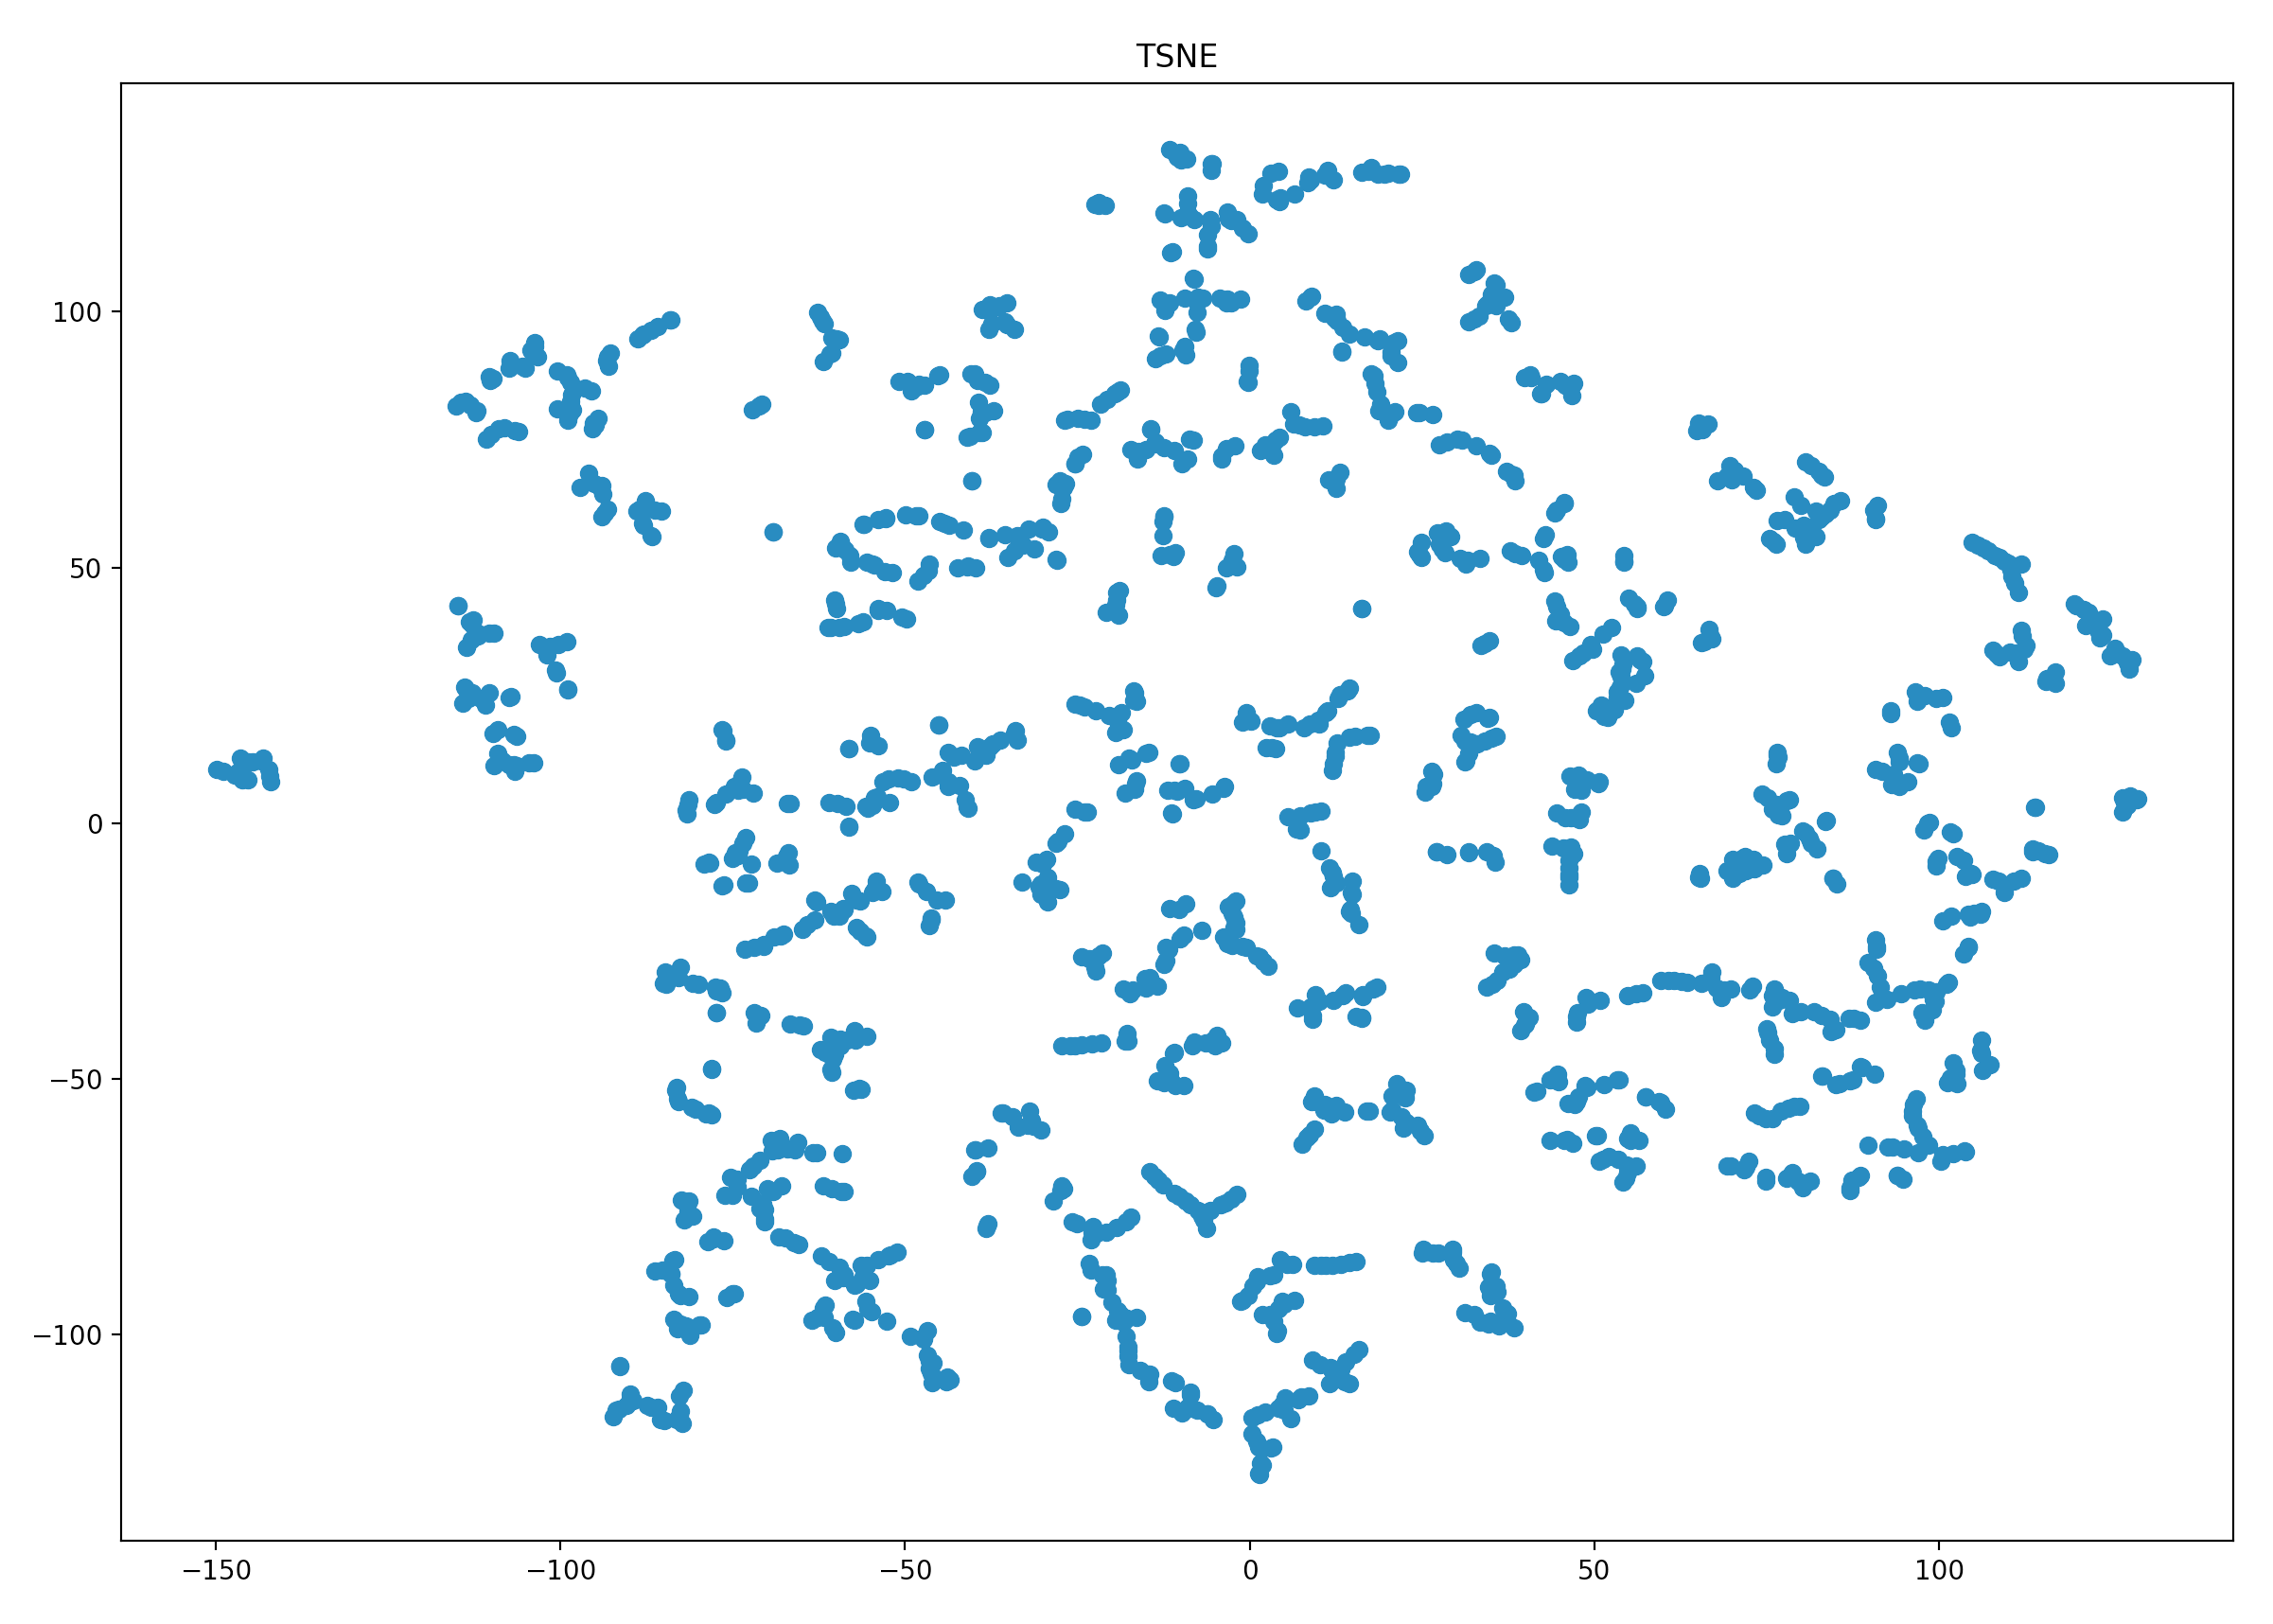
\includegraphics[width=0.9\textwidth]{./images/tsneParametersTest/perplexity/perp5-1hTSNE.png}
  % \caption{}
  % \label{figure:}
  \end{subfigure}%
  \begin{subfigure}{.5\textwidth}
    \centering
    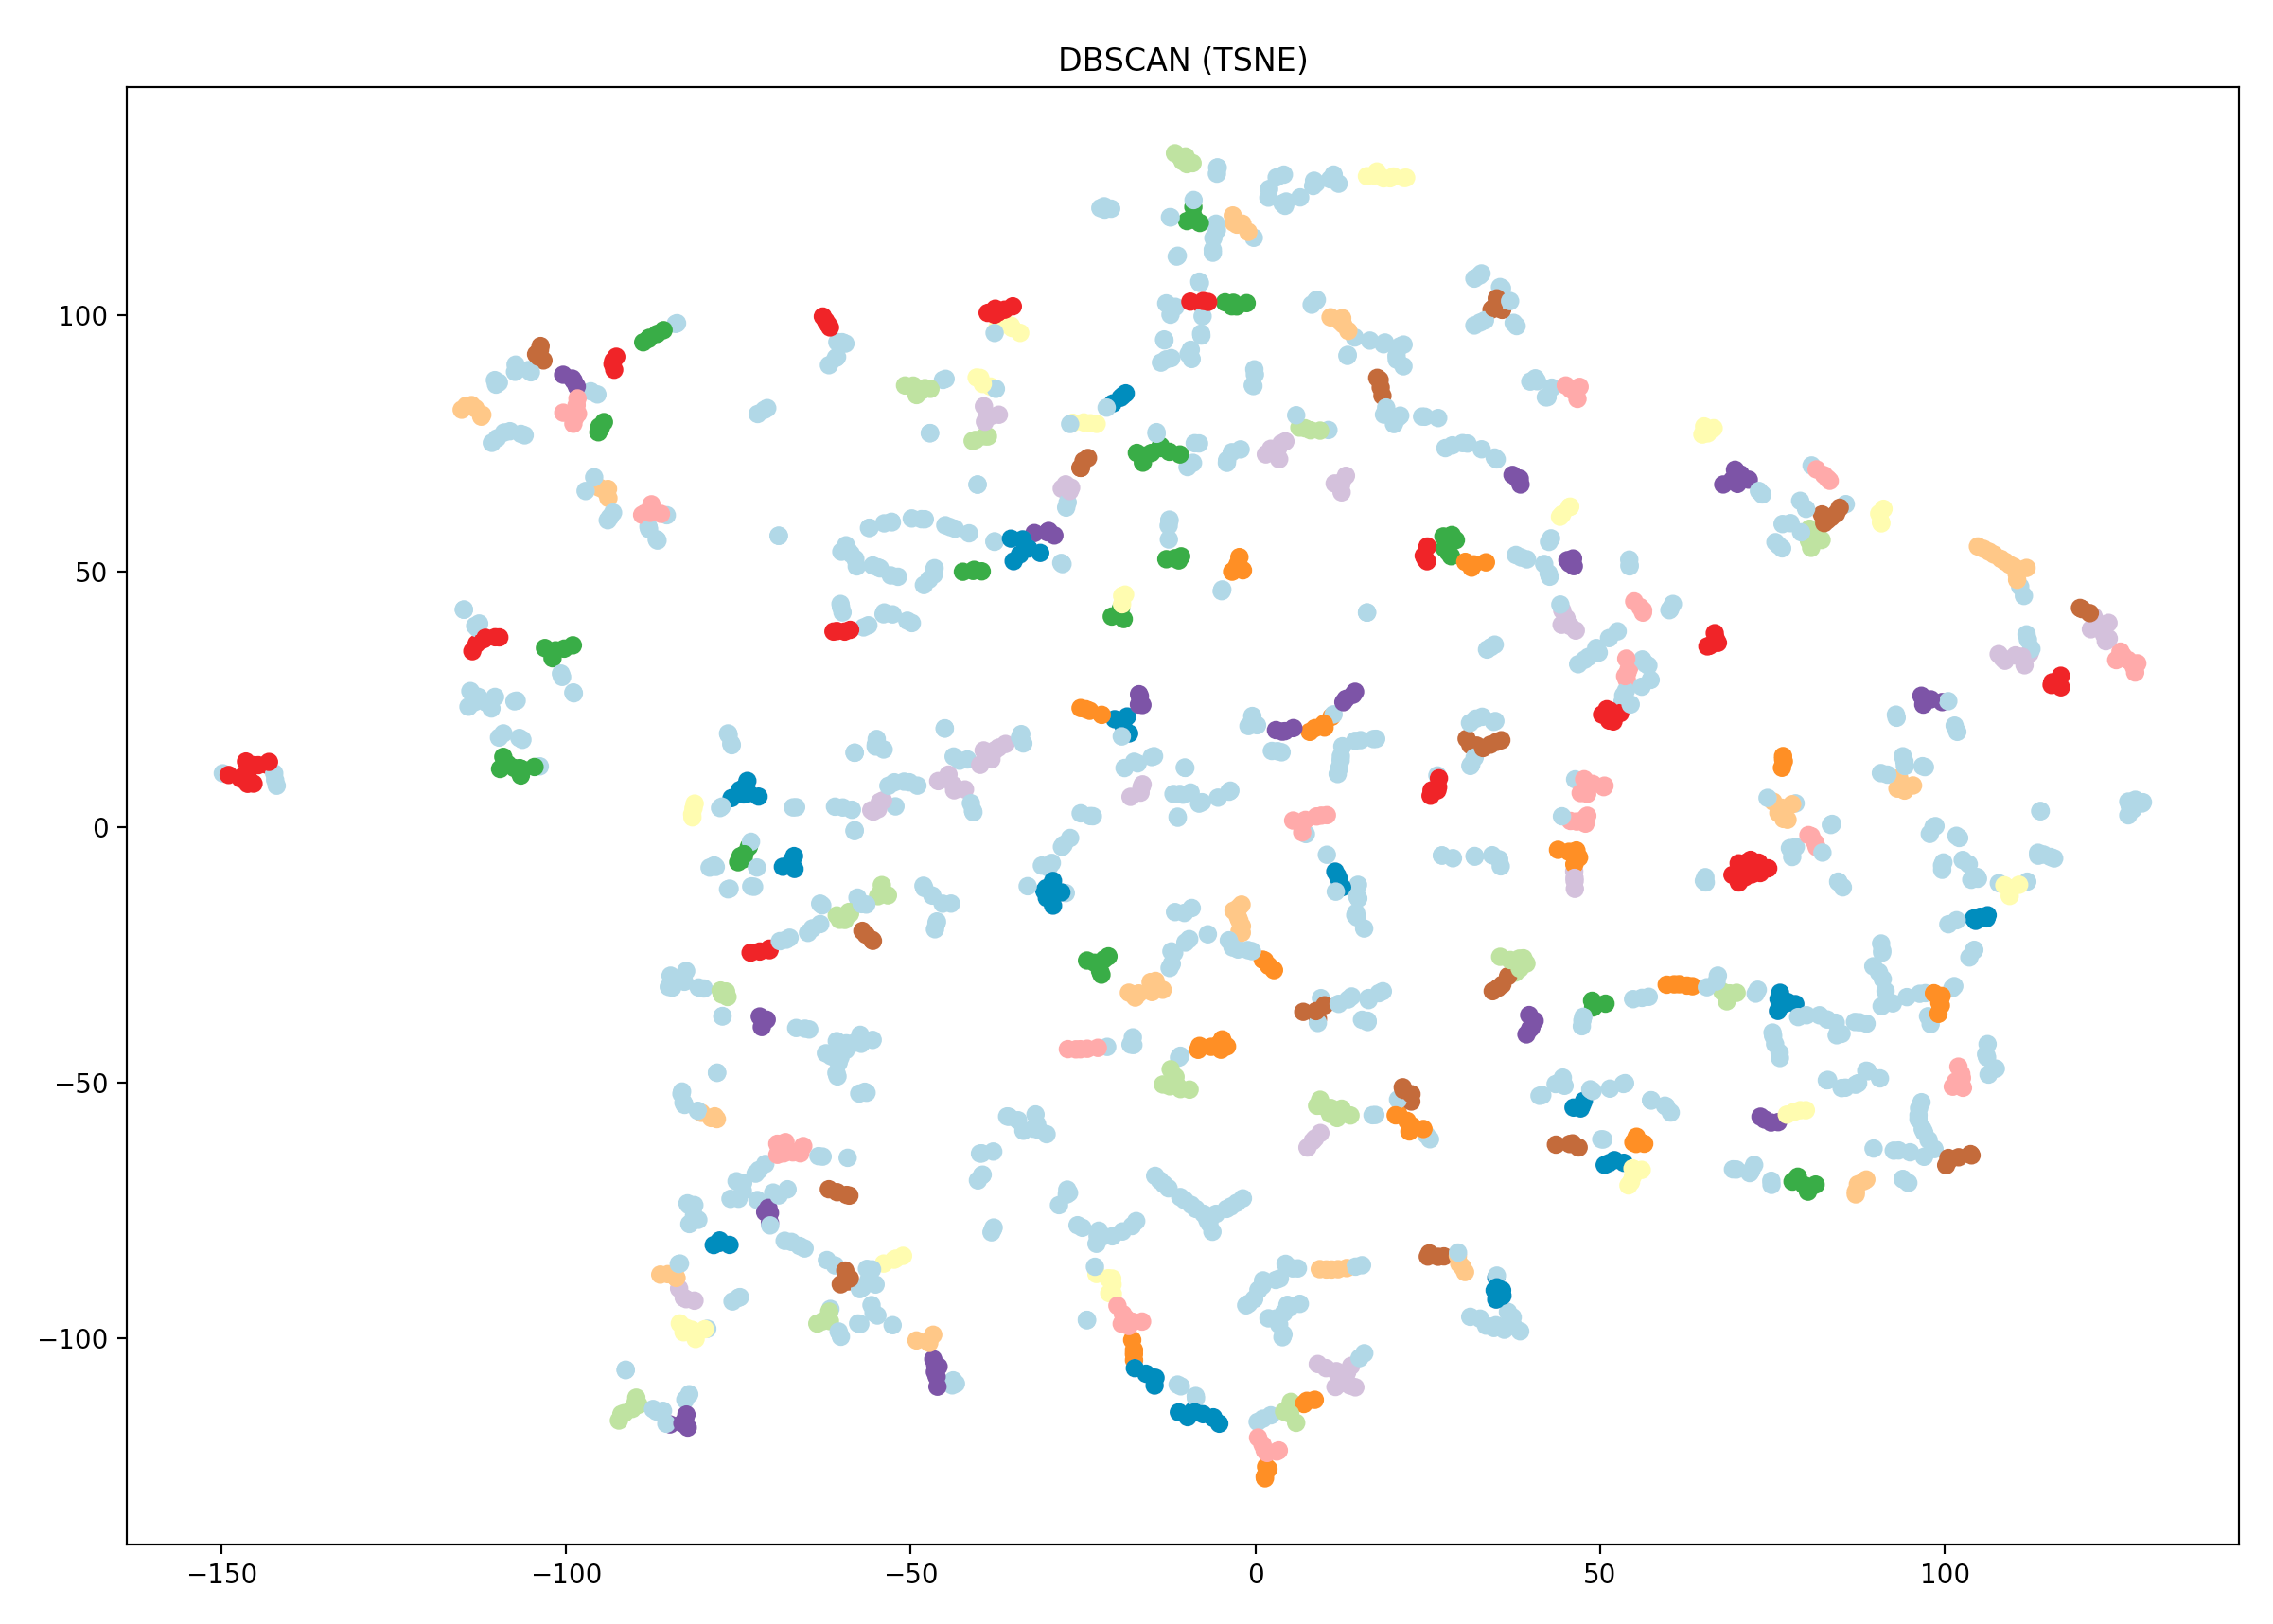
\includegraphics[width=0.9\textwidth]{./images/tsneParametersTest/perplexity/perp5-1hDBSCAN.png}
    % \caption{}
    % \label{figure:}
  \end{subfigure}
	\caption{\textbf{1h} data files, t-SNE calculated with the following parameters: \textbf{perplexity=5}, n\_iter=5000, learning\_rate=50}
	\label{figure:1hperp5TSNE}
\end{figure}


% -- 3h, perp 5 --
\begin{figure}[H]
	\centering
	
  \centering
	\begin{subfigure}{.5\textwidth}
    \centering
    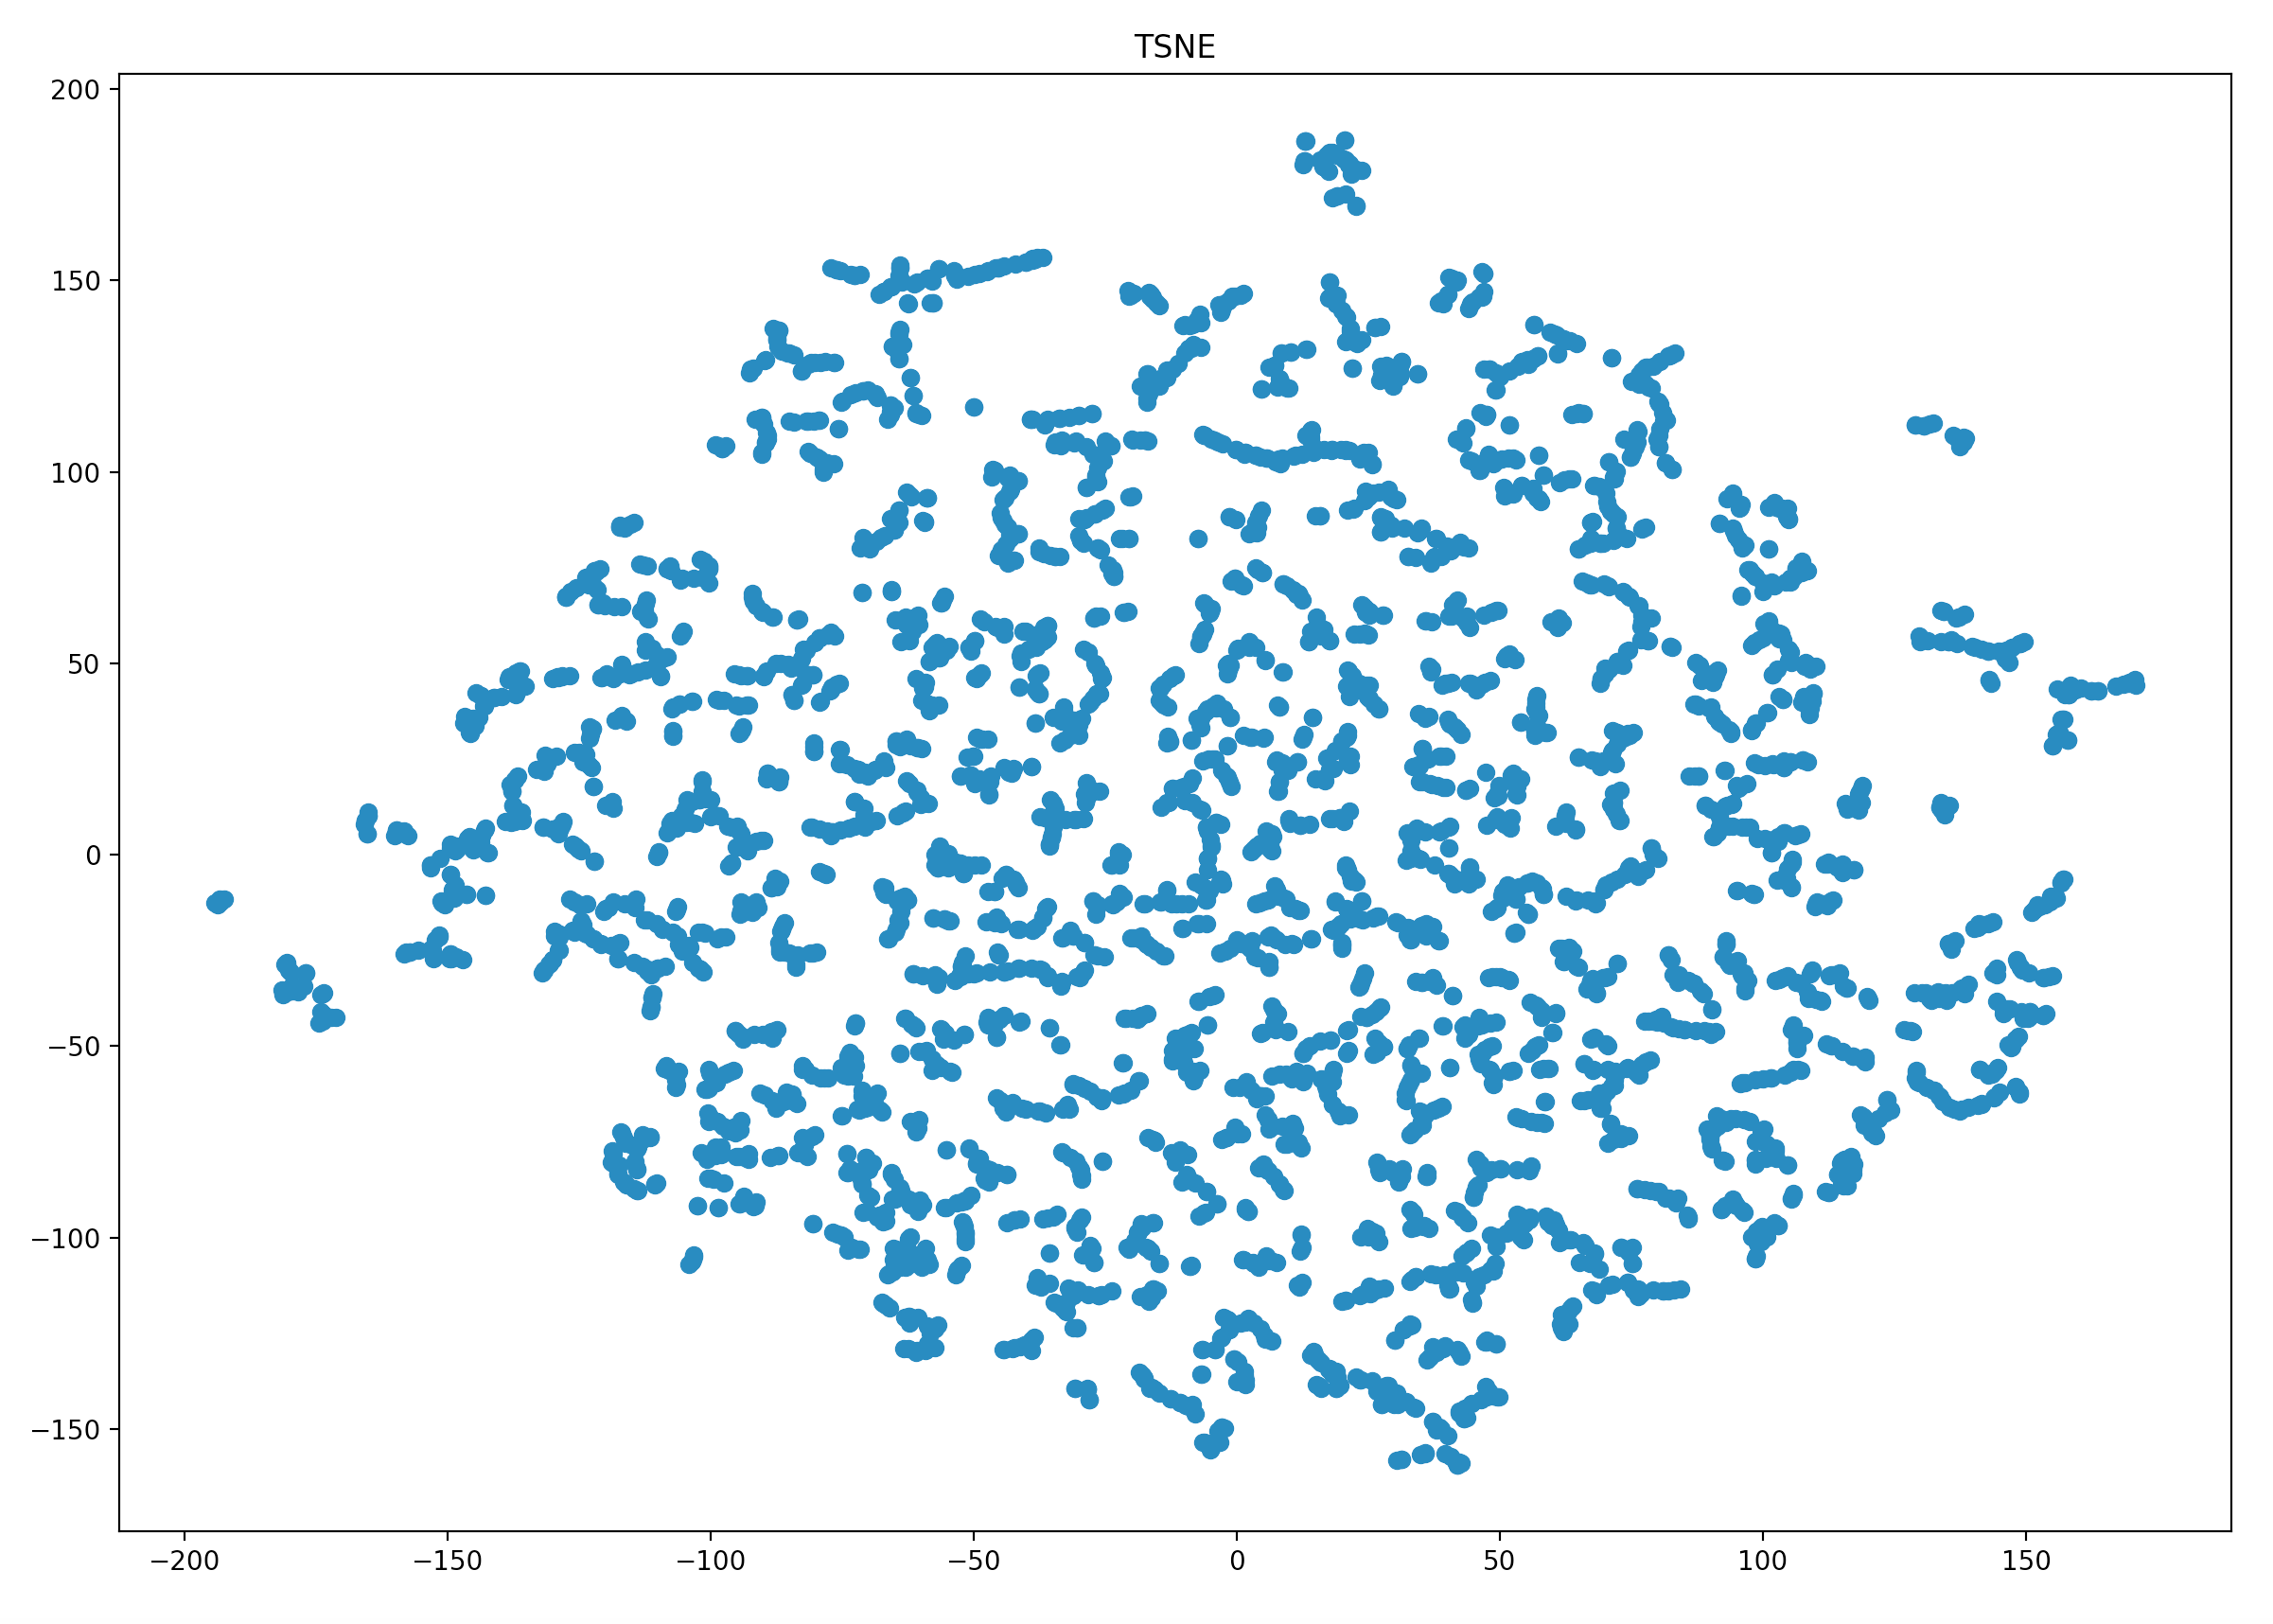
\includegraphics[width=0.9\textwidth]{./images/tsneParametersTest/perplexity/perp5-3hTSNE.png}
  % \caption{}
  % \label{figure:}
  \end{subfigure}%
  \begin{subfigure}{.5\textwidth}
    \centering
    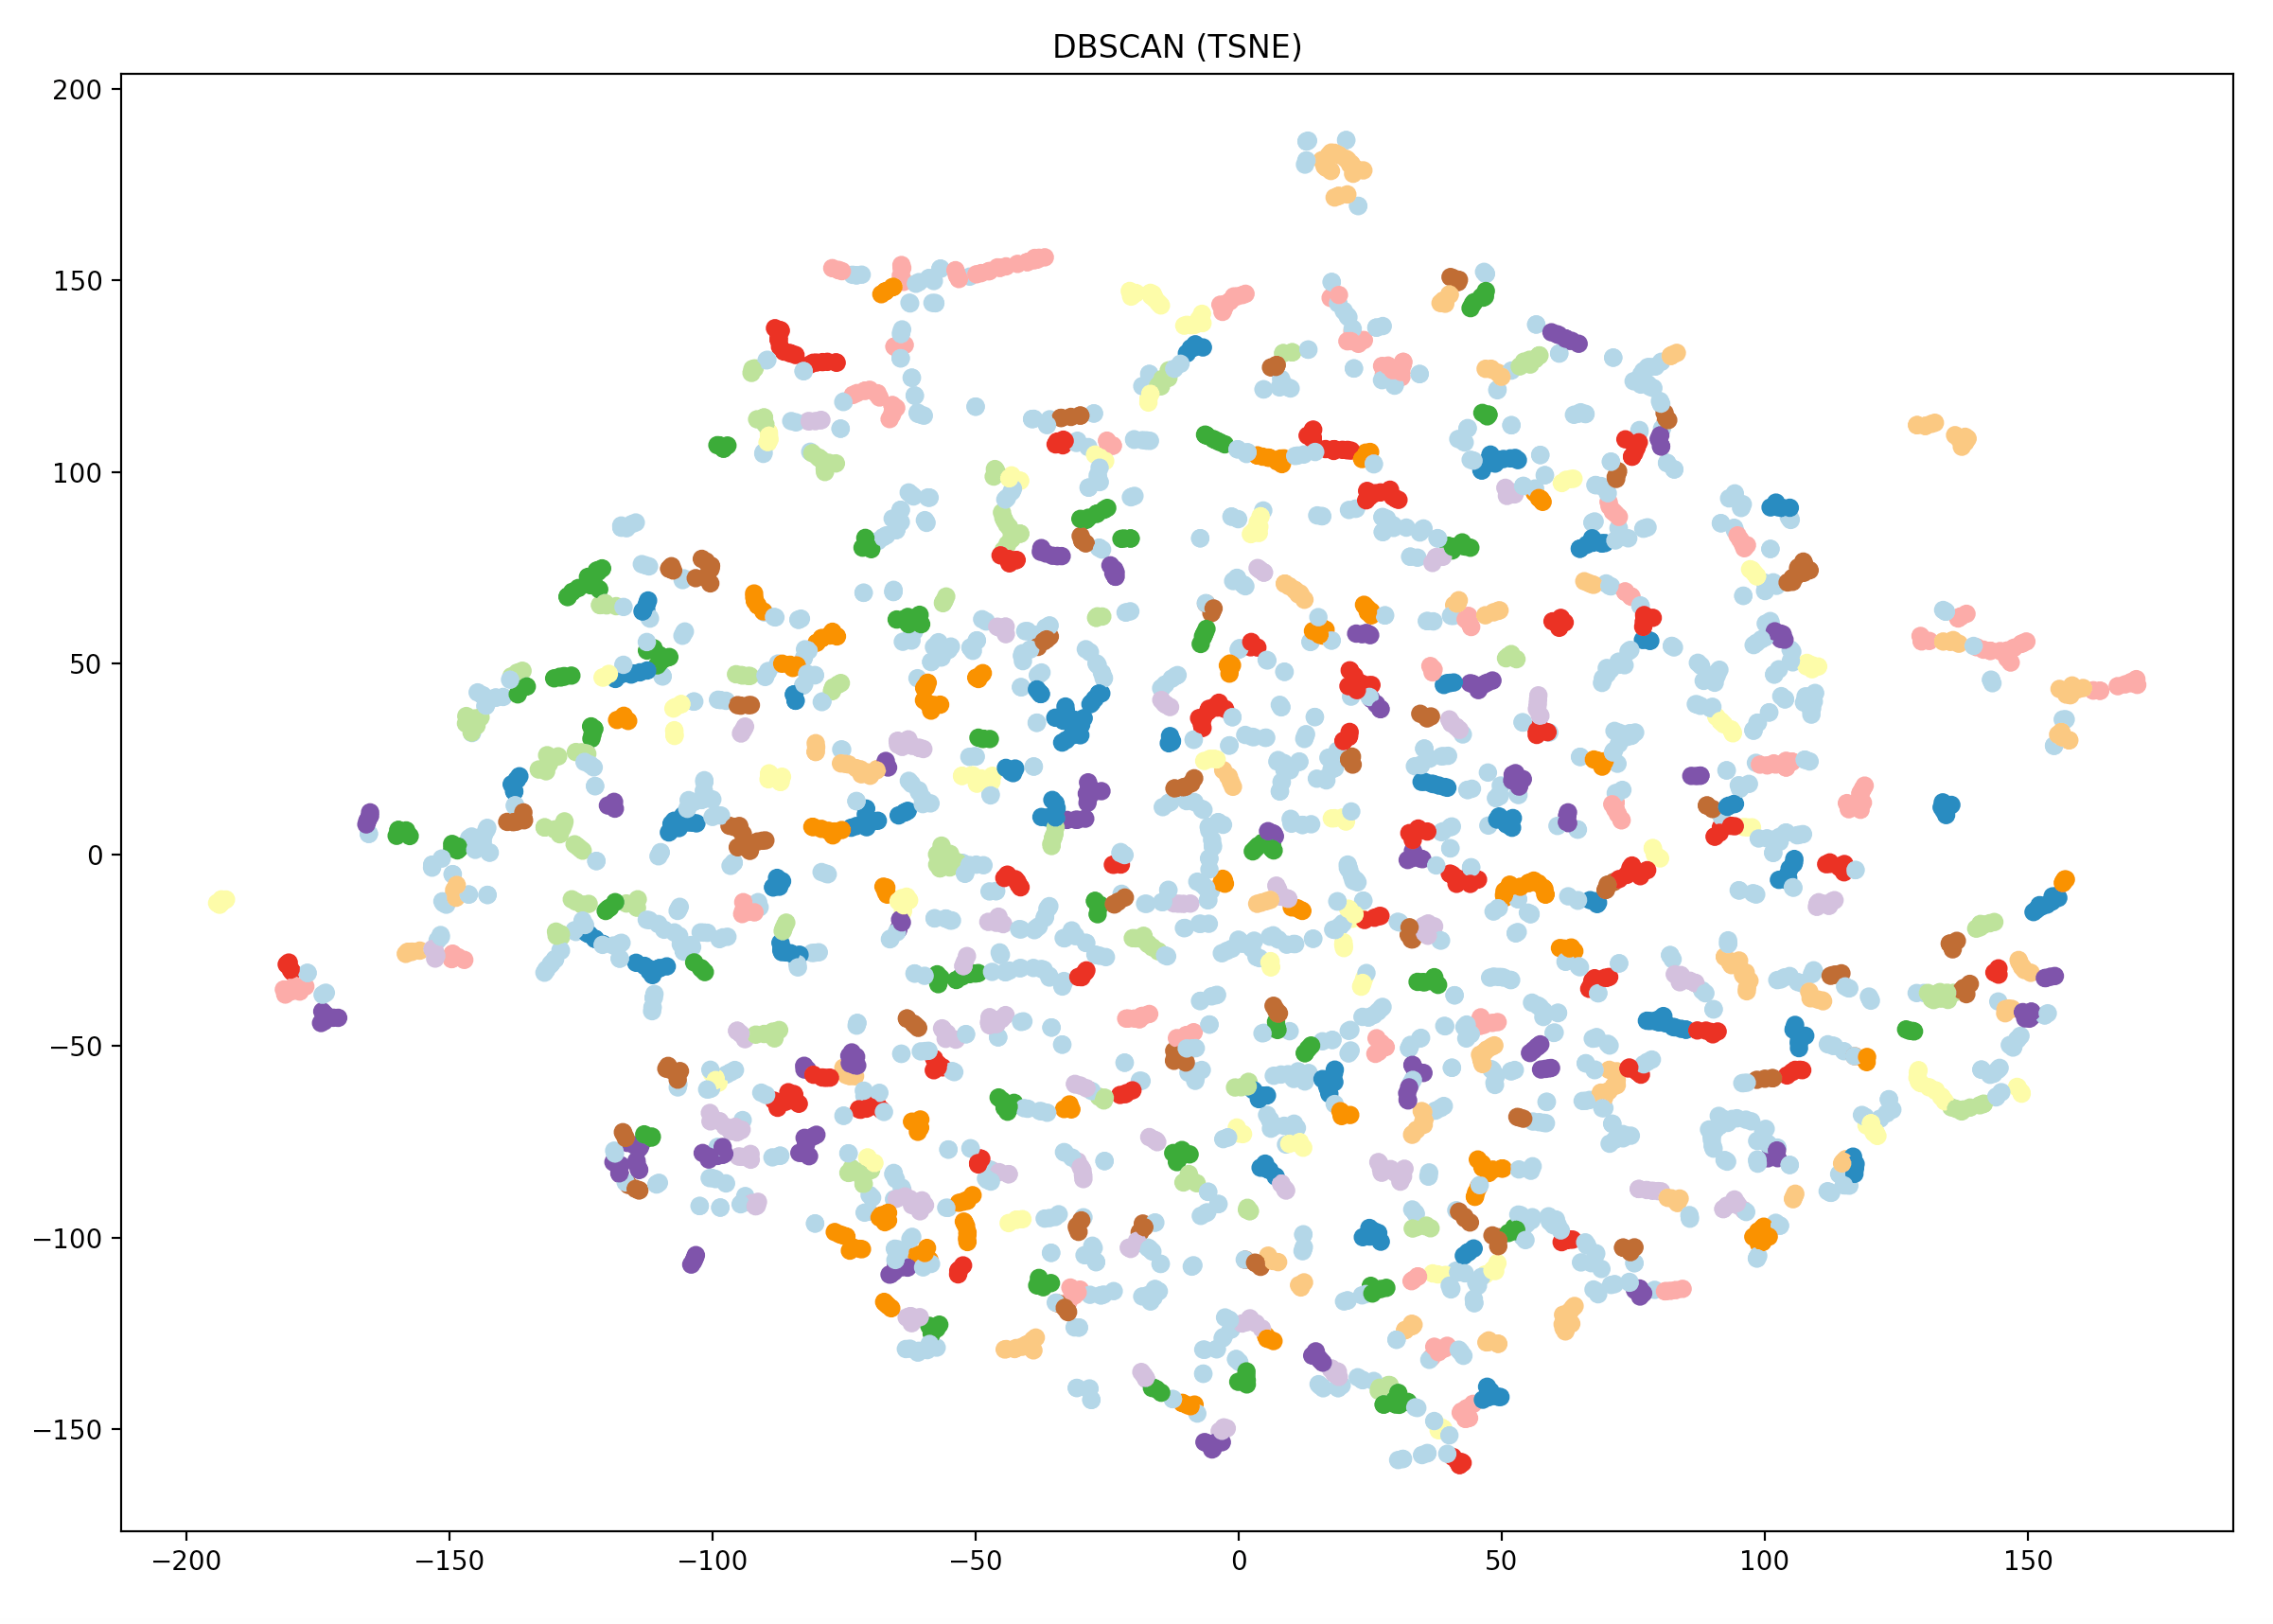
\includegraphics[width=0.9\textwidth]{./images/tsneParametersTest/perplexity/perp5-3hDBSCAN.png}
    % \caption{}
    % \label{figure:}
	\end{subfigure}
	\caption{\textbf{3h} data files, t-SNE calculated with the following parameters: \textbf{perplexity=5}, n\_iter=5000, learning\_rate=50}
  \label{figure:3hperp5TSNE}
\end{figure}


%------------------ PERPLEXITY 10: ------------------
\subsubsection{Perplexity = 10}
% -- 1h, perp 10 --
\begin{figure}[H]
  \centering
  \begin{subfigure}{.5\textwidth}
    \centering
    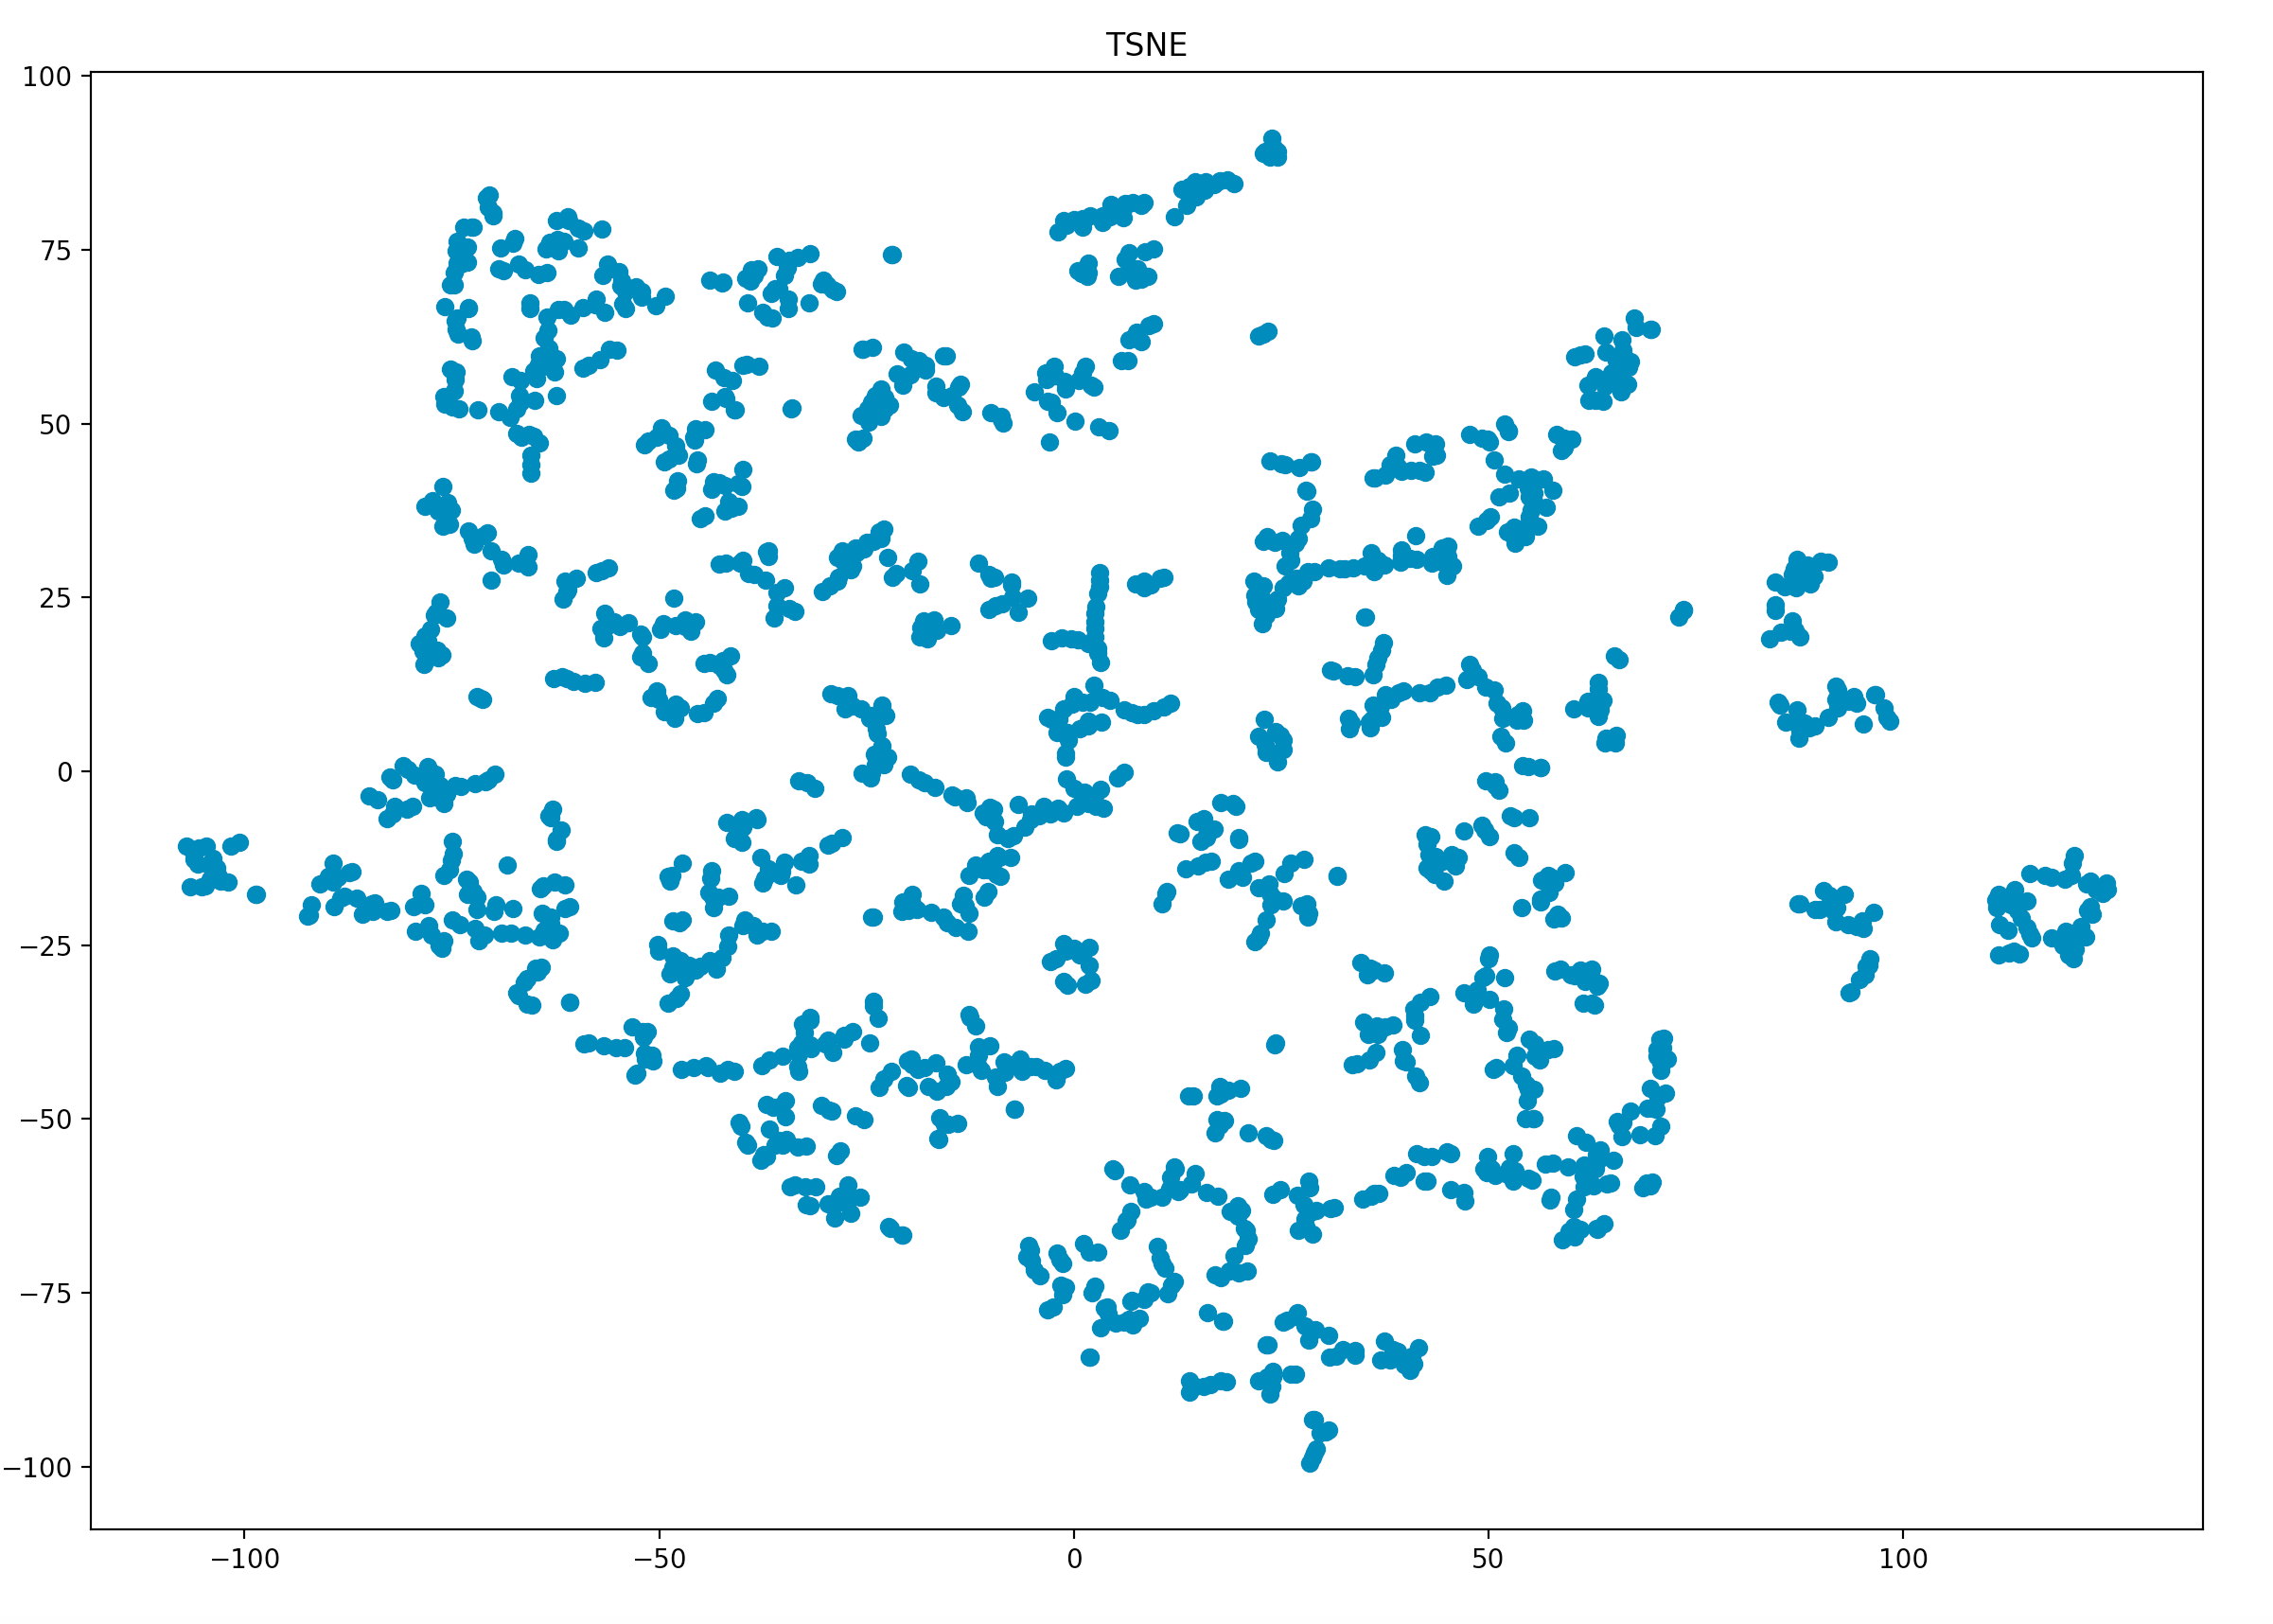
\includegraphics[width=0.9\textwidth]{./images/tsneParametersTest/perplexity/perp10-1hTSNE.png}
  % \caption{}
  % \label{figure:}
  \end{subfigure}%
  \begin{subfigure}{.5\textwidth}
    \centering
    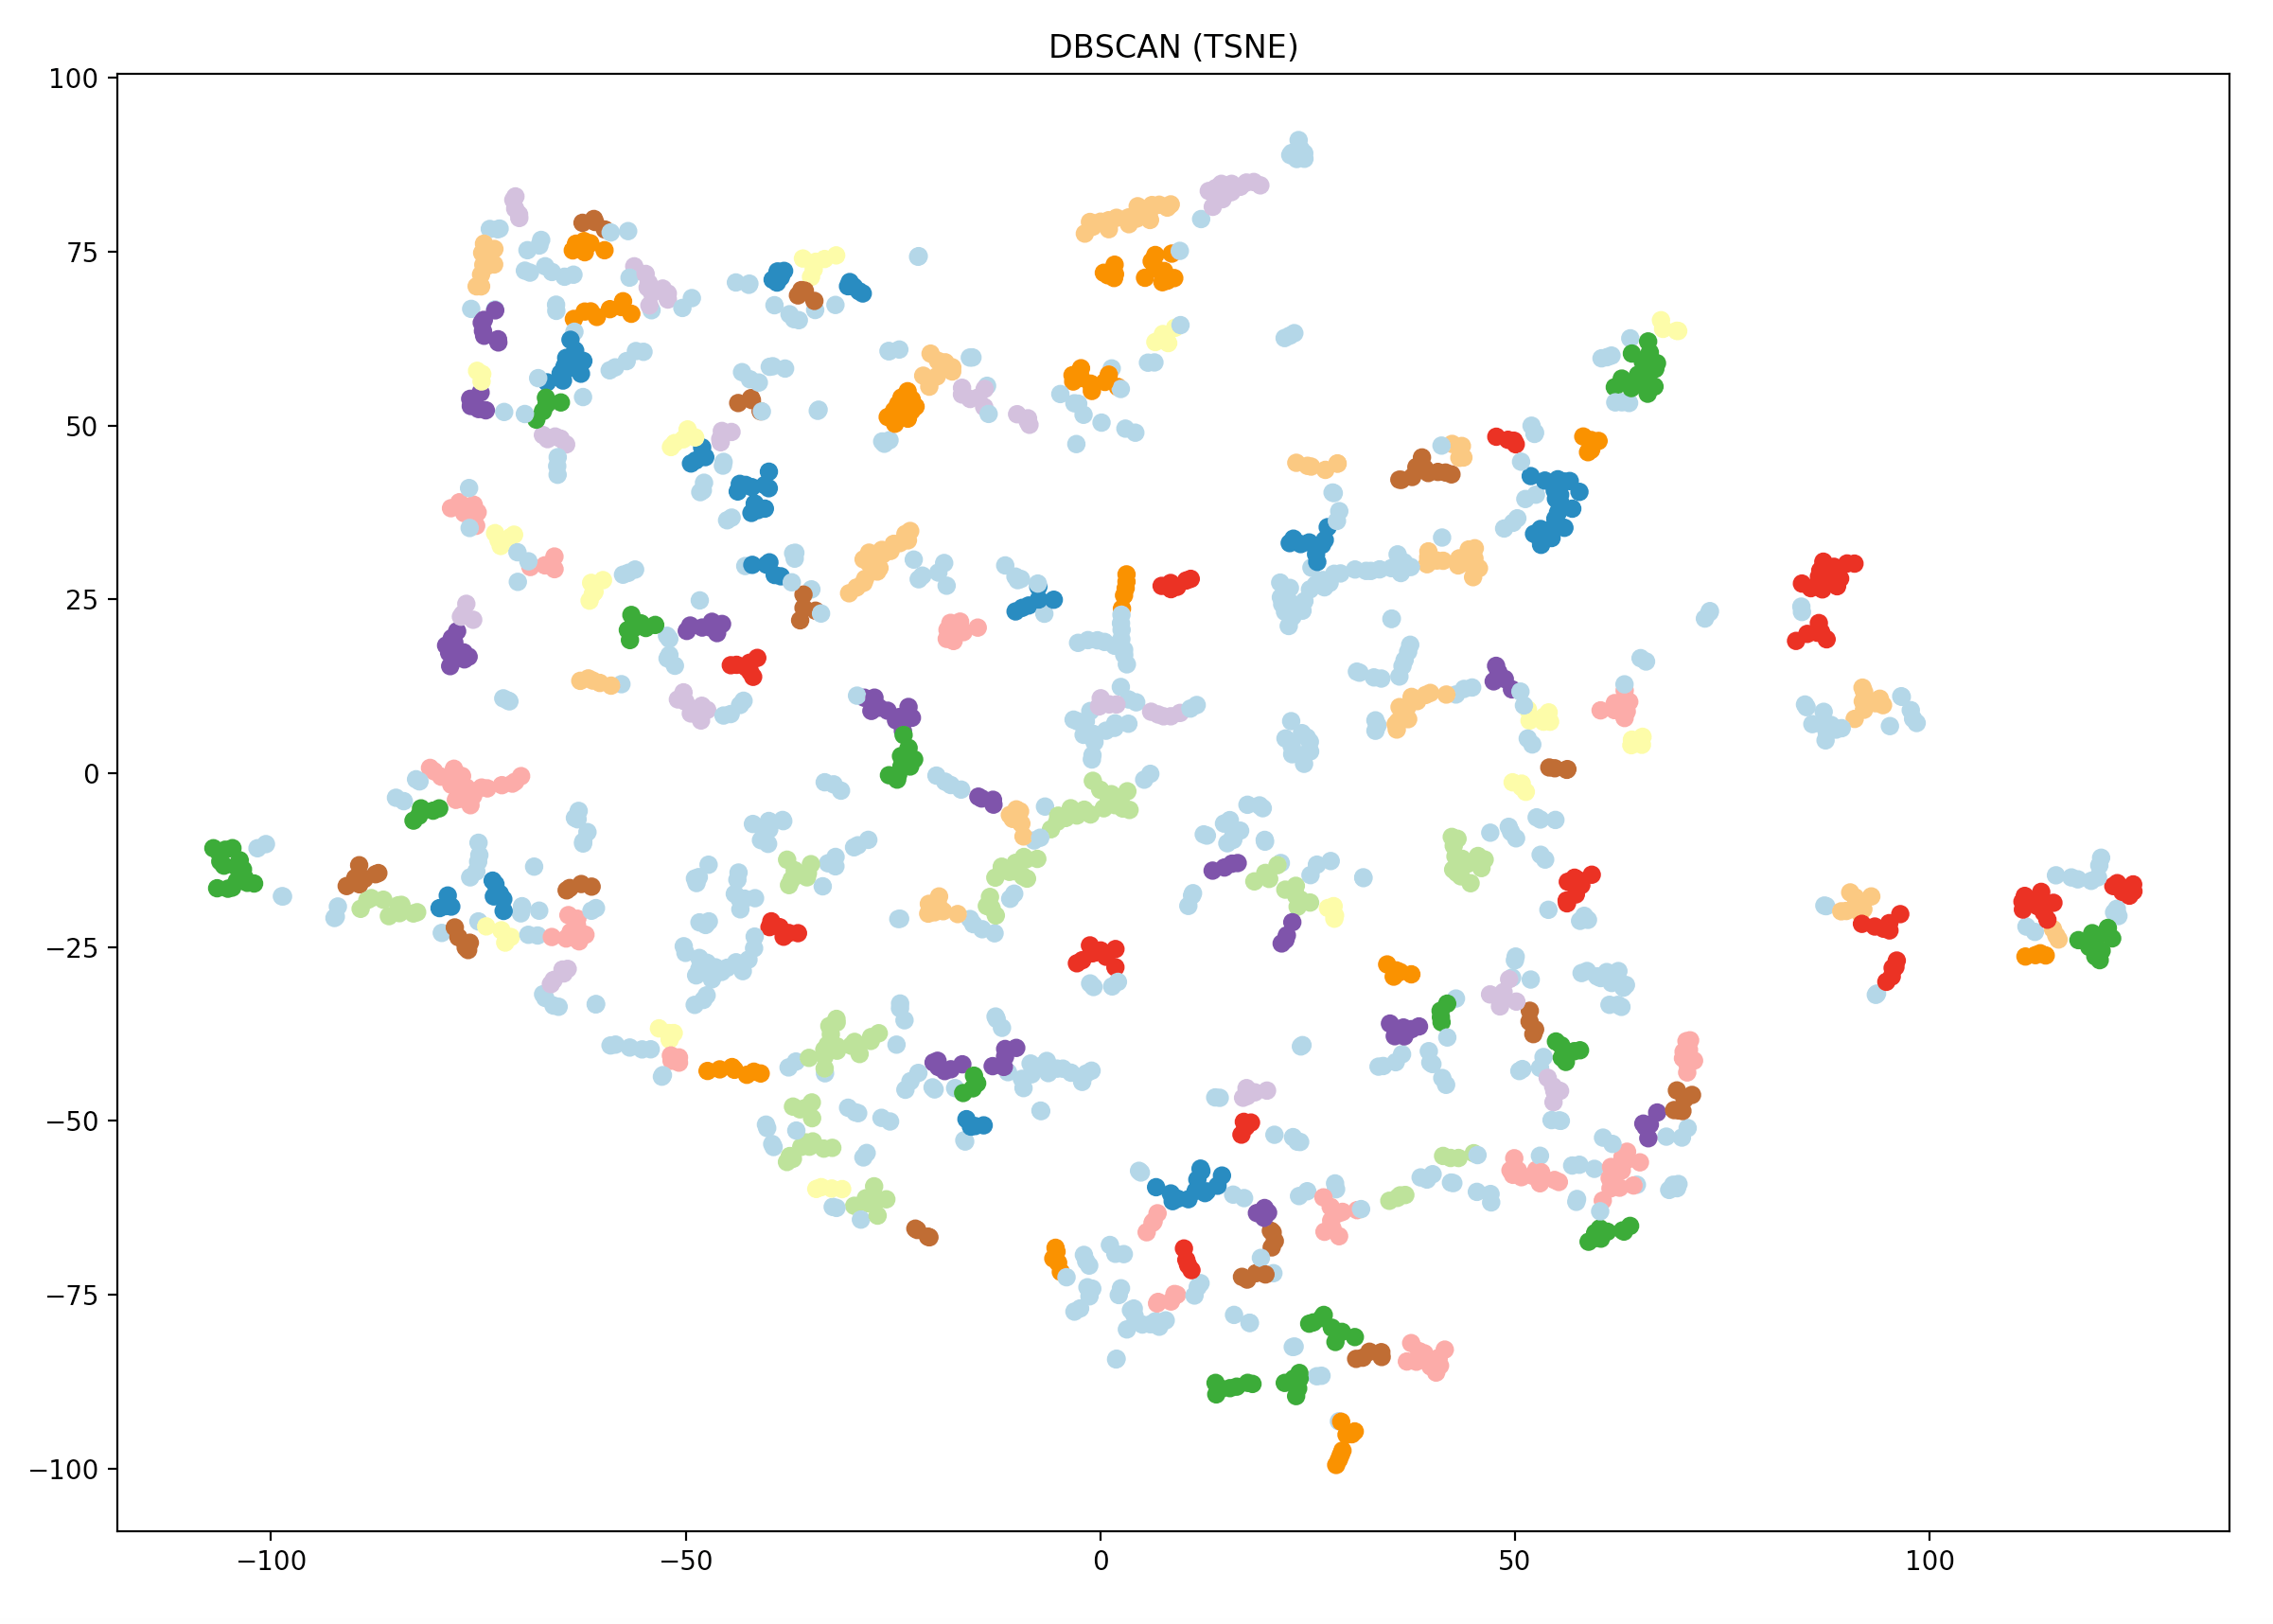
\includegraphics[width=0.9\textwidth]{./images/tsneParametersTest/perplexity/perp10-1hDBSCAN.png}
    % \caption{}
    % \label{figure:}
  \end{subfigure}
	\caption{\textbf{1h} data files, t-SNE calculated with the following parameters: \textbf{perplexity=10}, n\_iter=5000, learning\_rate=50}
  \label{figure:1hperp10TSNE}
\end{figure}

% -- 3h, perp 10 --
\begin{figure}[H]
  \centering
	\begin{subfigure}{.5\textwidth}
    \centering
    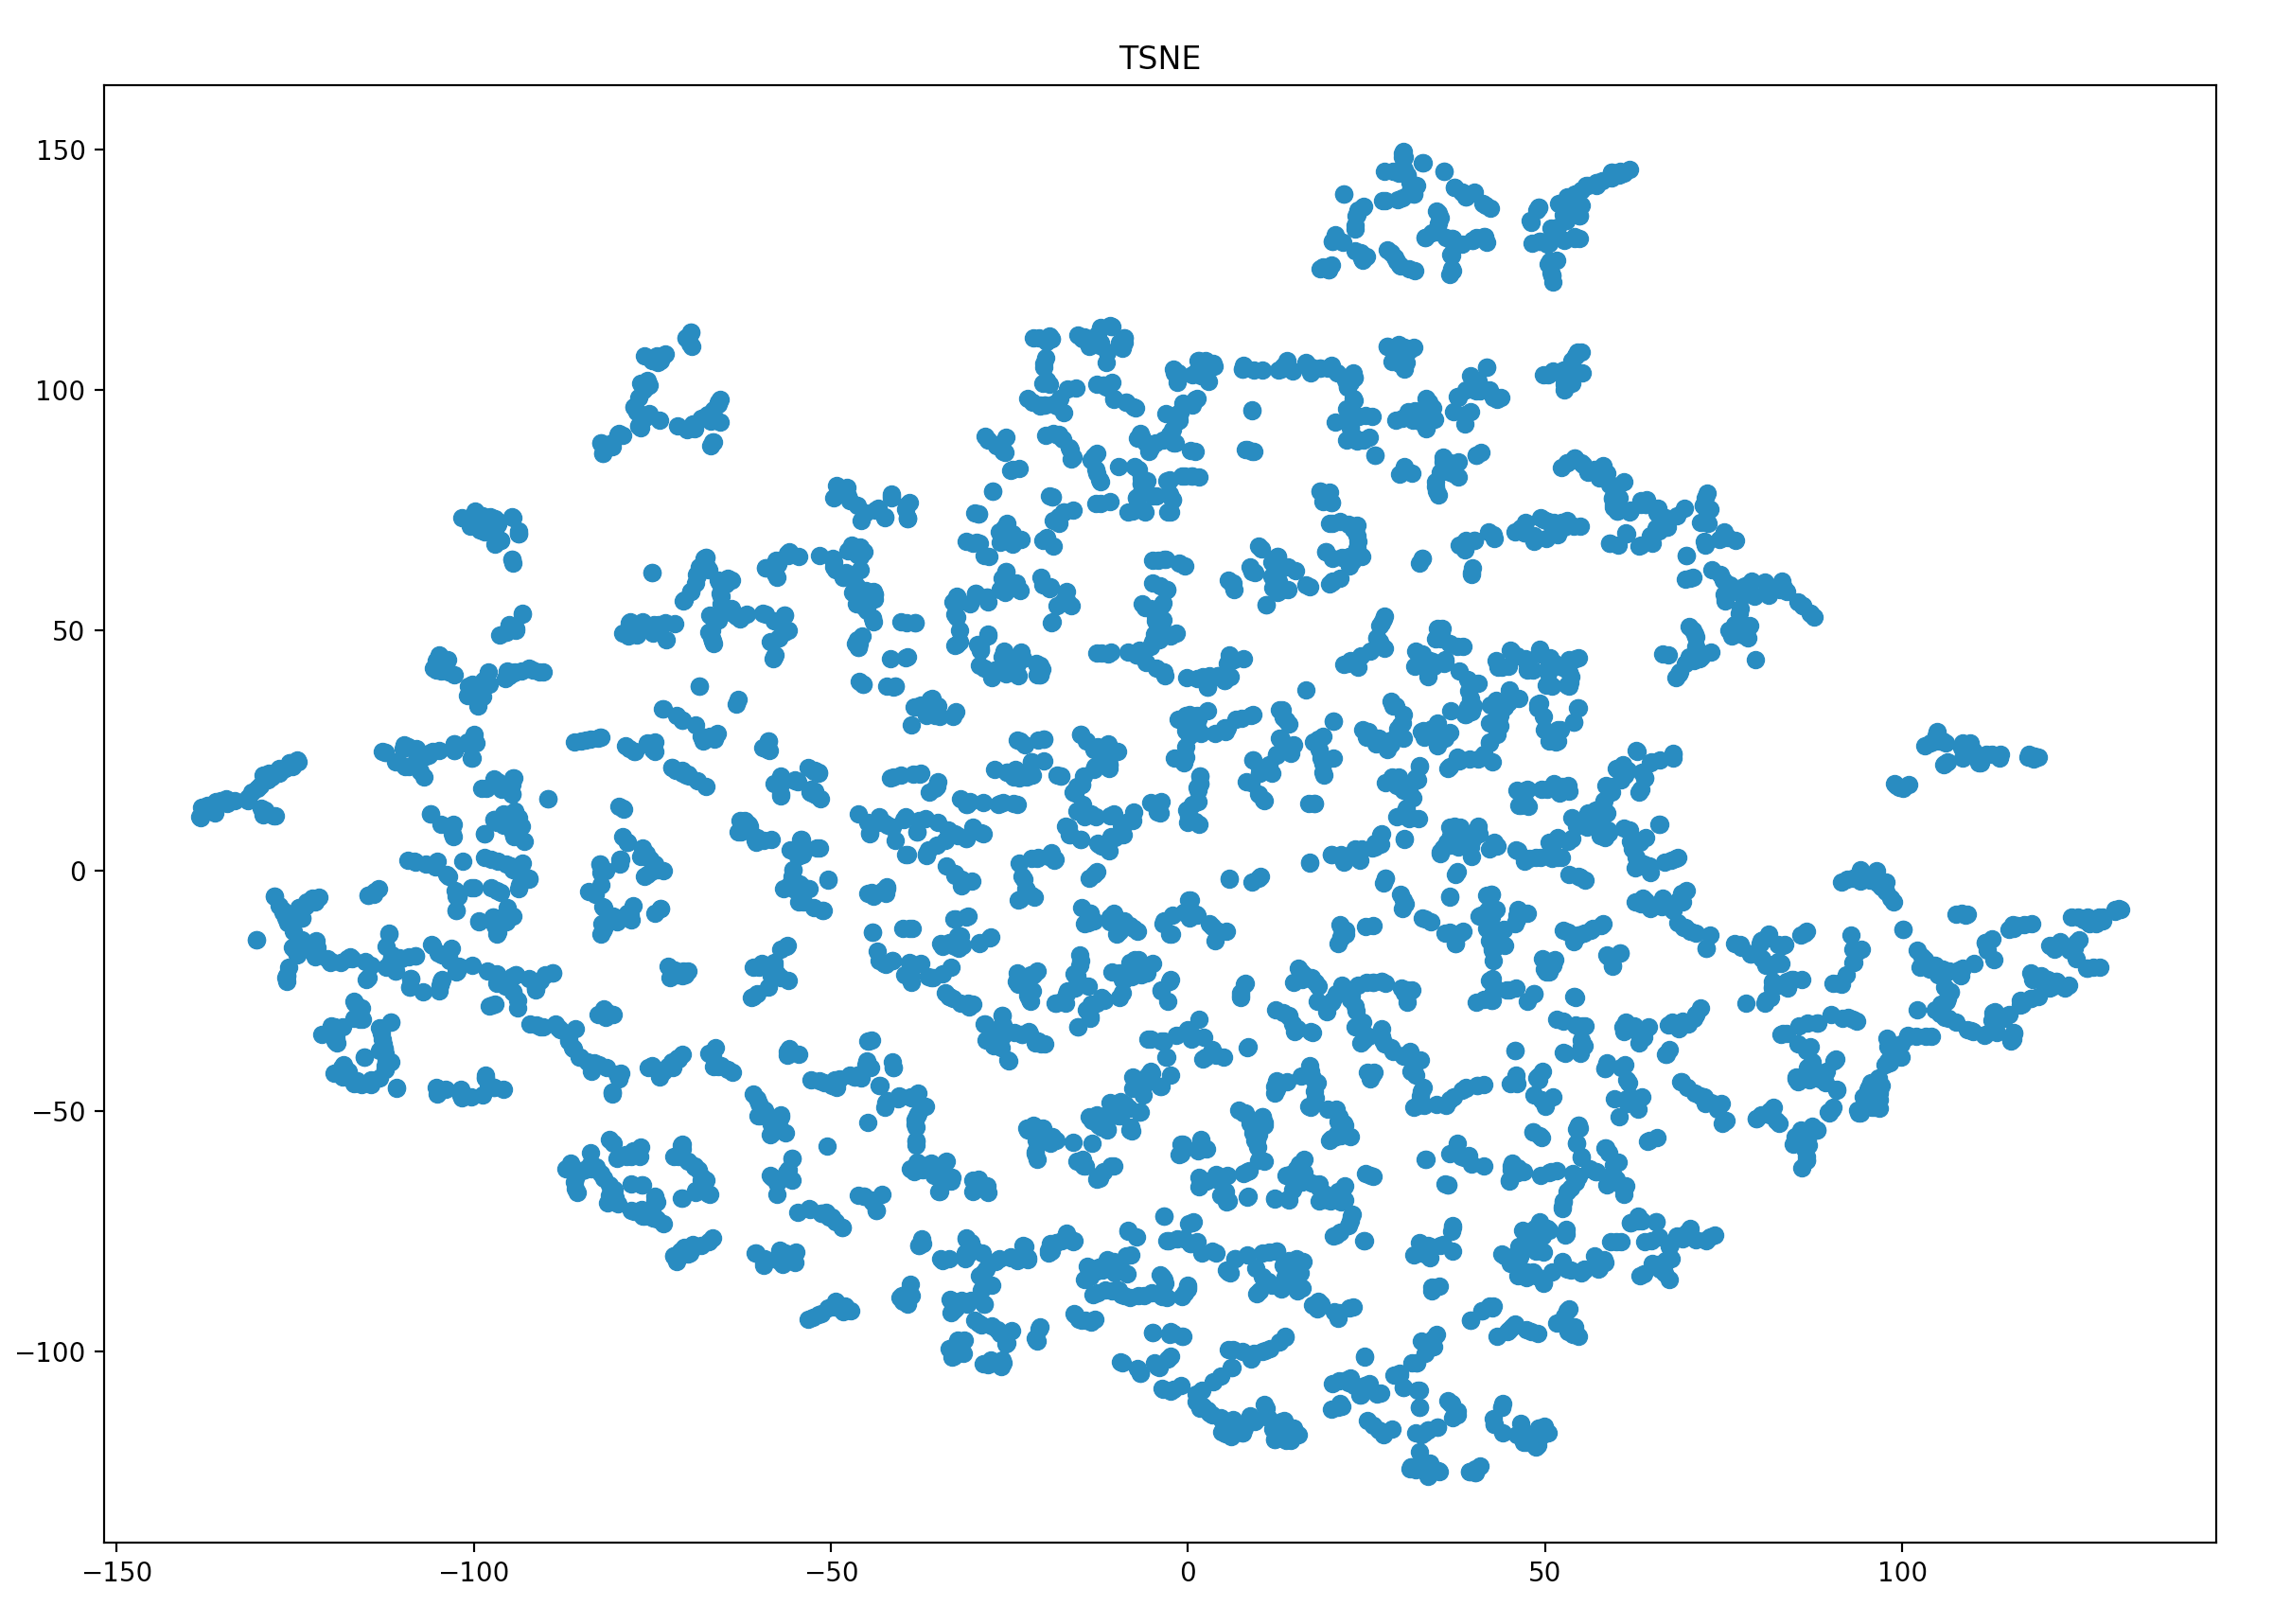
\includegraphics[width=0.9\textwidth]{./images/tsneParametersTest/perplexity/perp10-3hTSNE.png}
  % \caption{}
  % \label{figure:}
  \end{subfigure}%
  \begin{subfigure}{.5\textwidth}
    \centering
    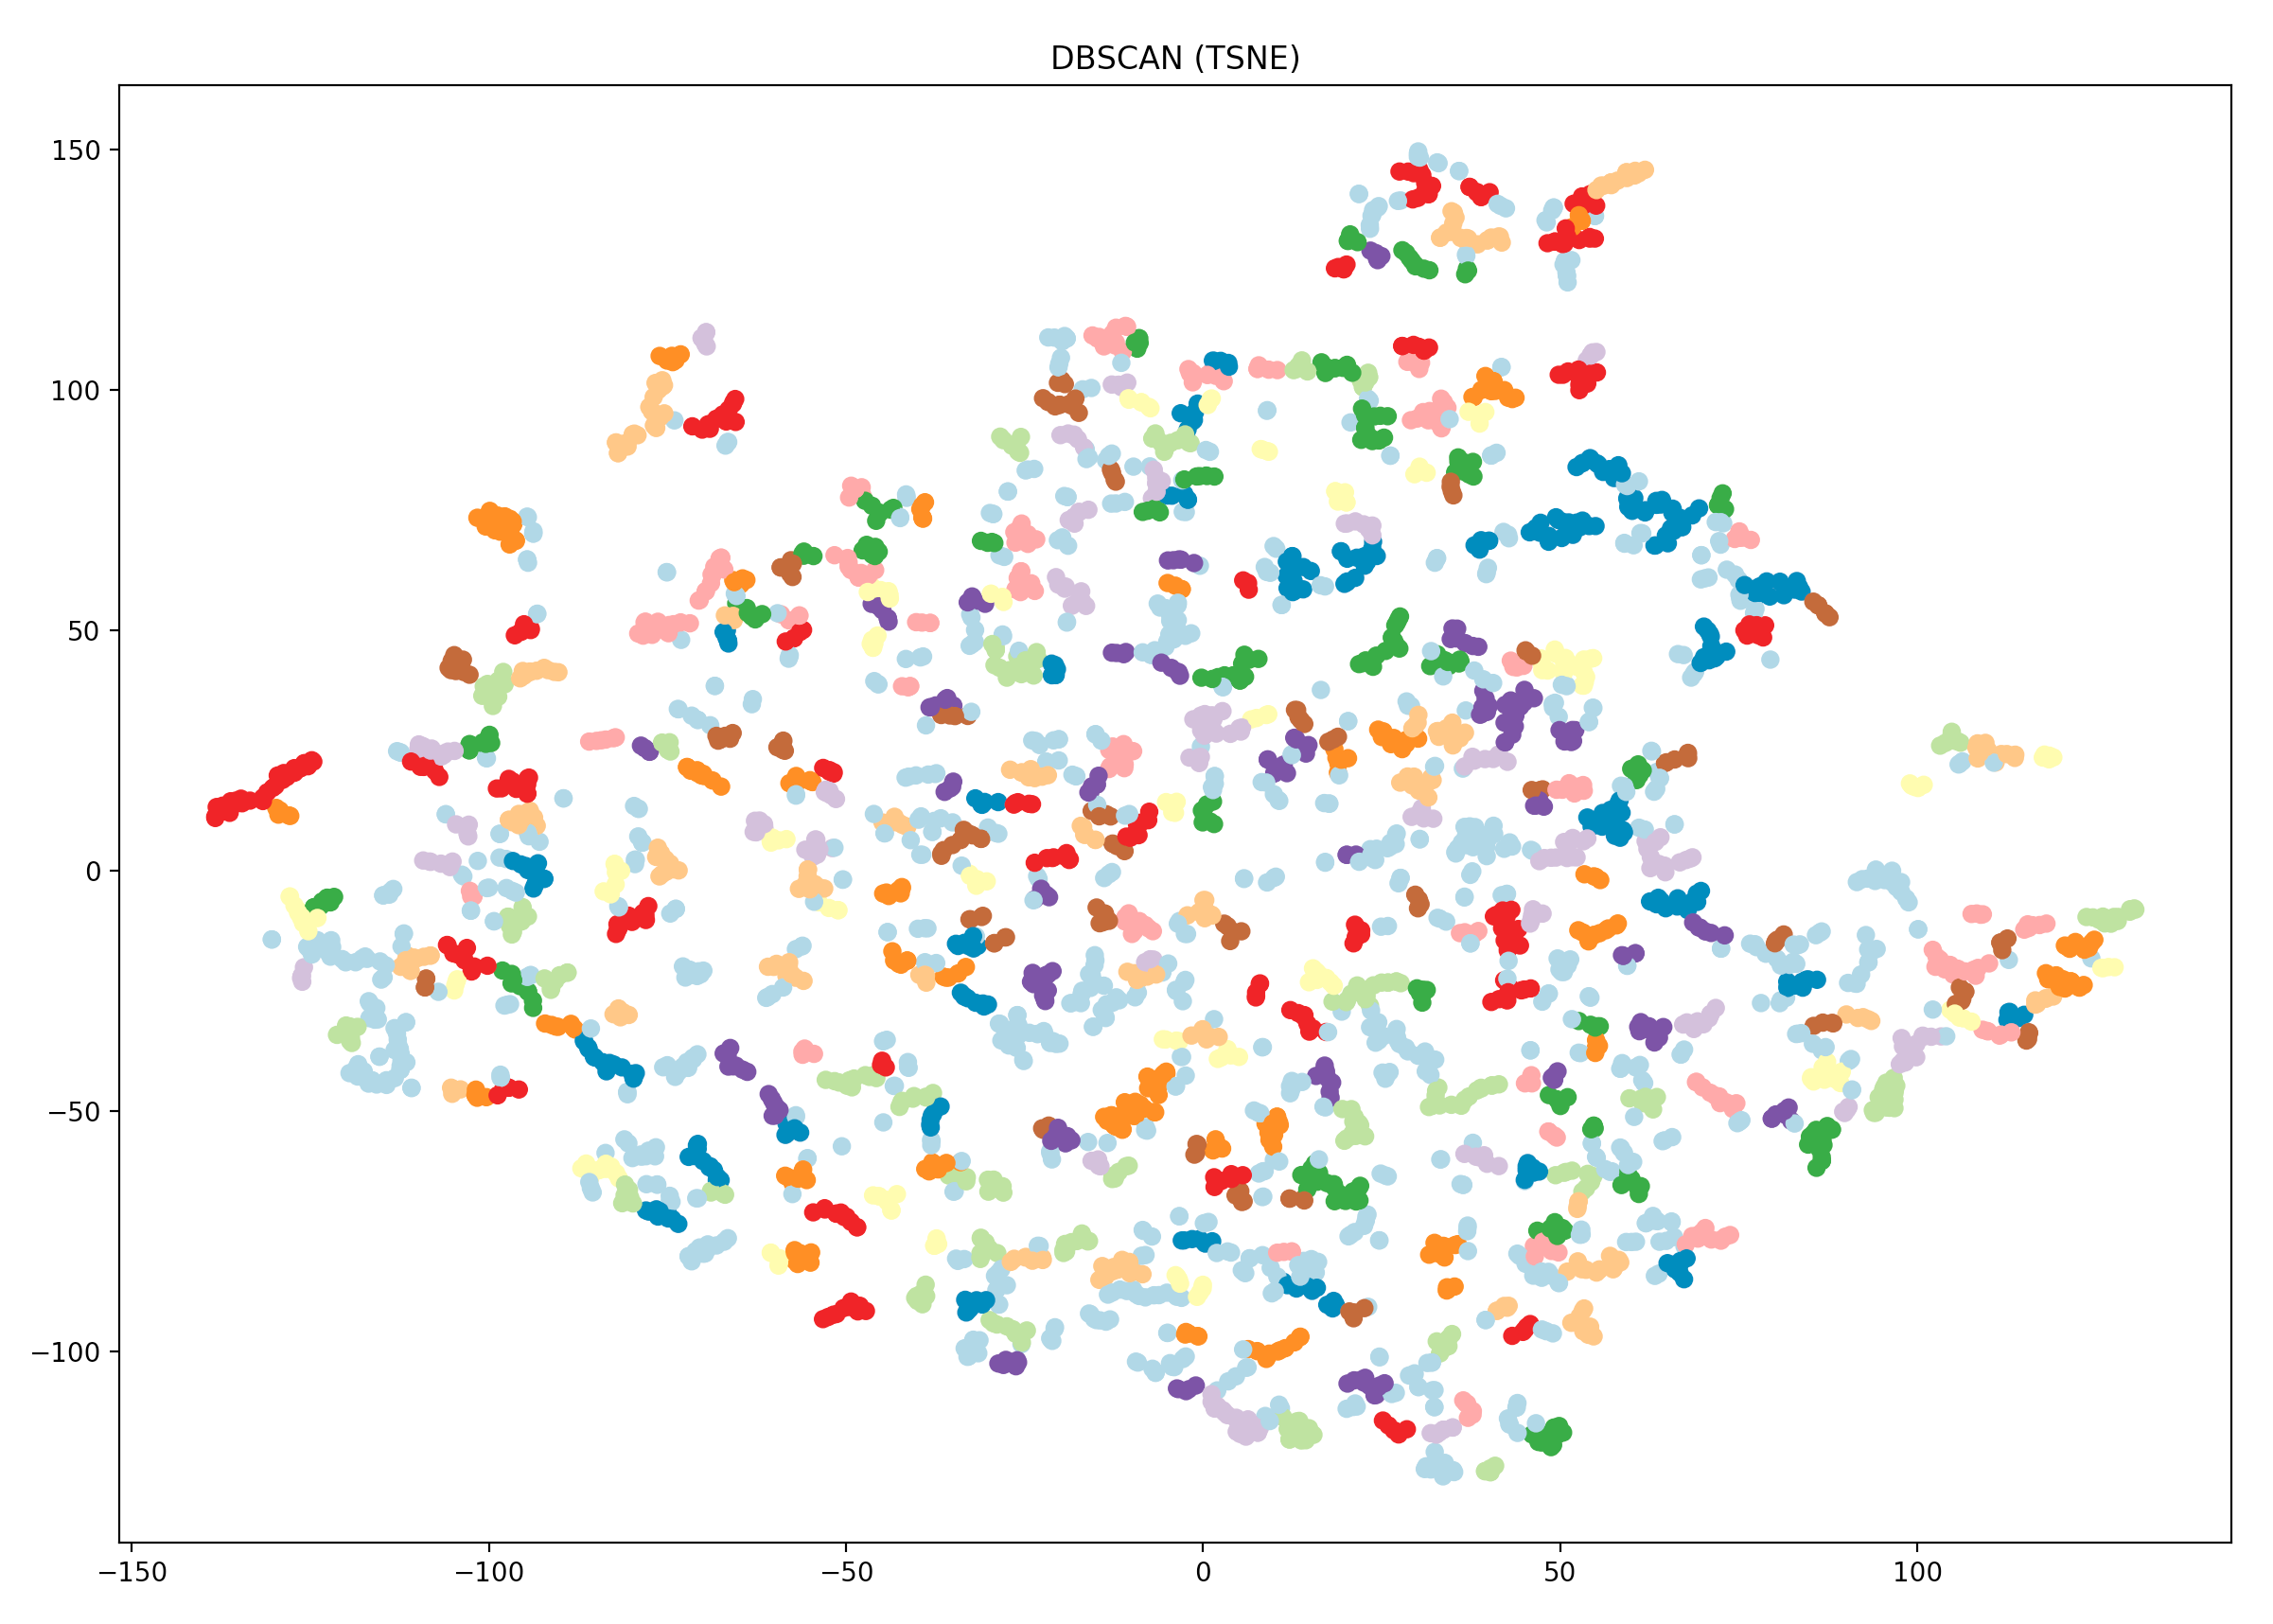
\includegraphics[width=0.9\textwidth]{./images/tsneParametersTest/perplexity/perp10-3hDBSCAN.png}
    % \caption{}
    % \label{figure:}
	\end{subfigure}
	\caption{\textbf{3h} data files, t-SNE calculated with the following parameters: \textbf{perplexity=10}, n\_iter=5000, learning\_rate=50}
  \label{figure:3hperp10TSNE}
\end{figure}

%------------------ PERPLEXITY 20: ------------------
\subsubsection{Perplexity = 20}
% -- 1h, perp 20 --
\begin{figure}[H]
  \centering
  \begin{subfigure}{.5\textwidth}
    \centering
    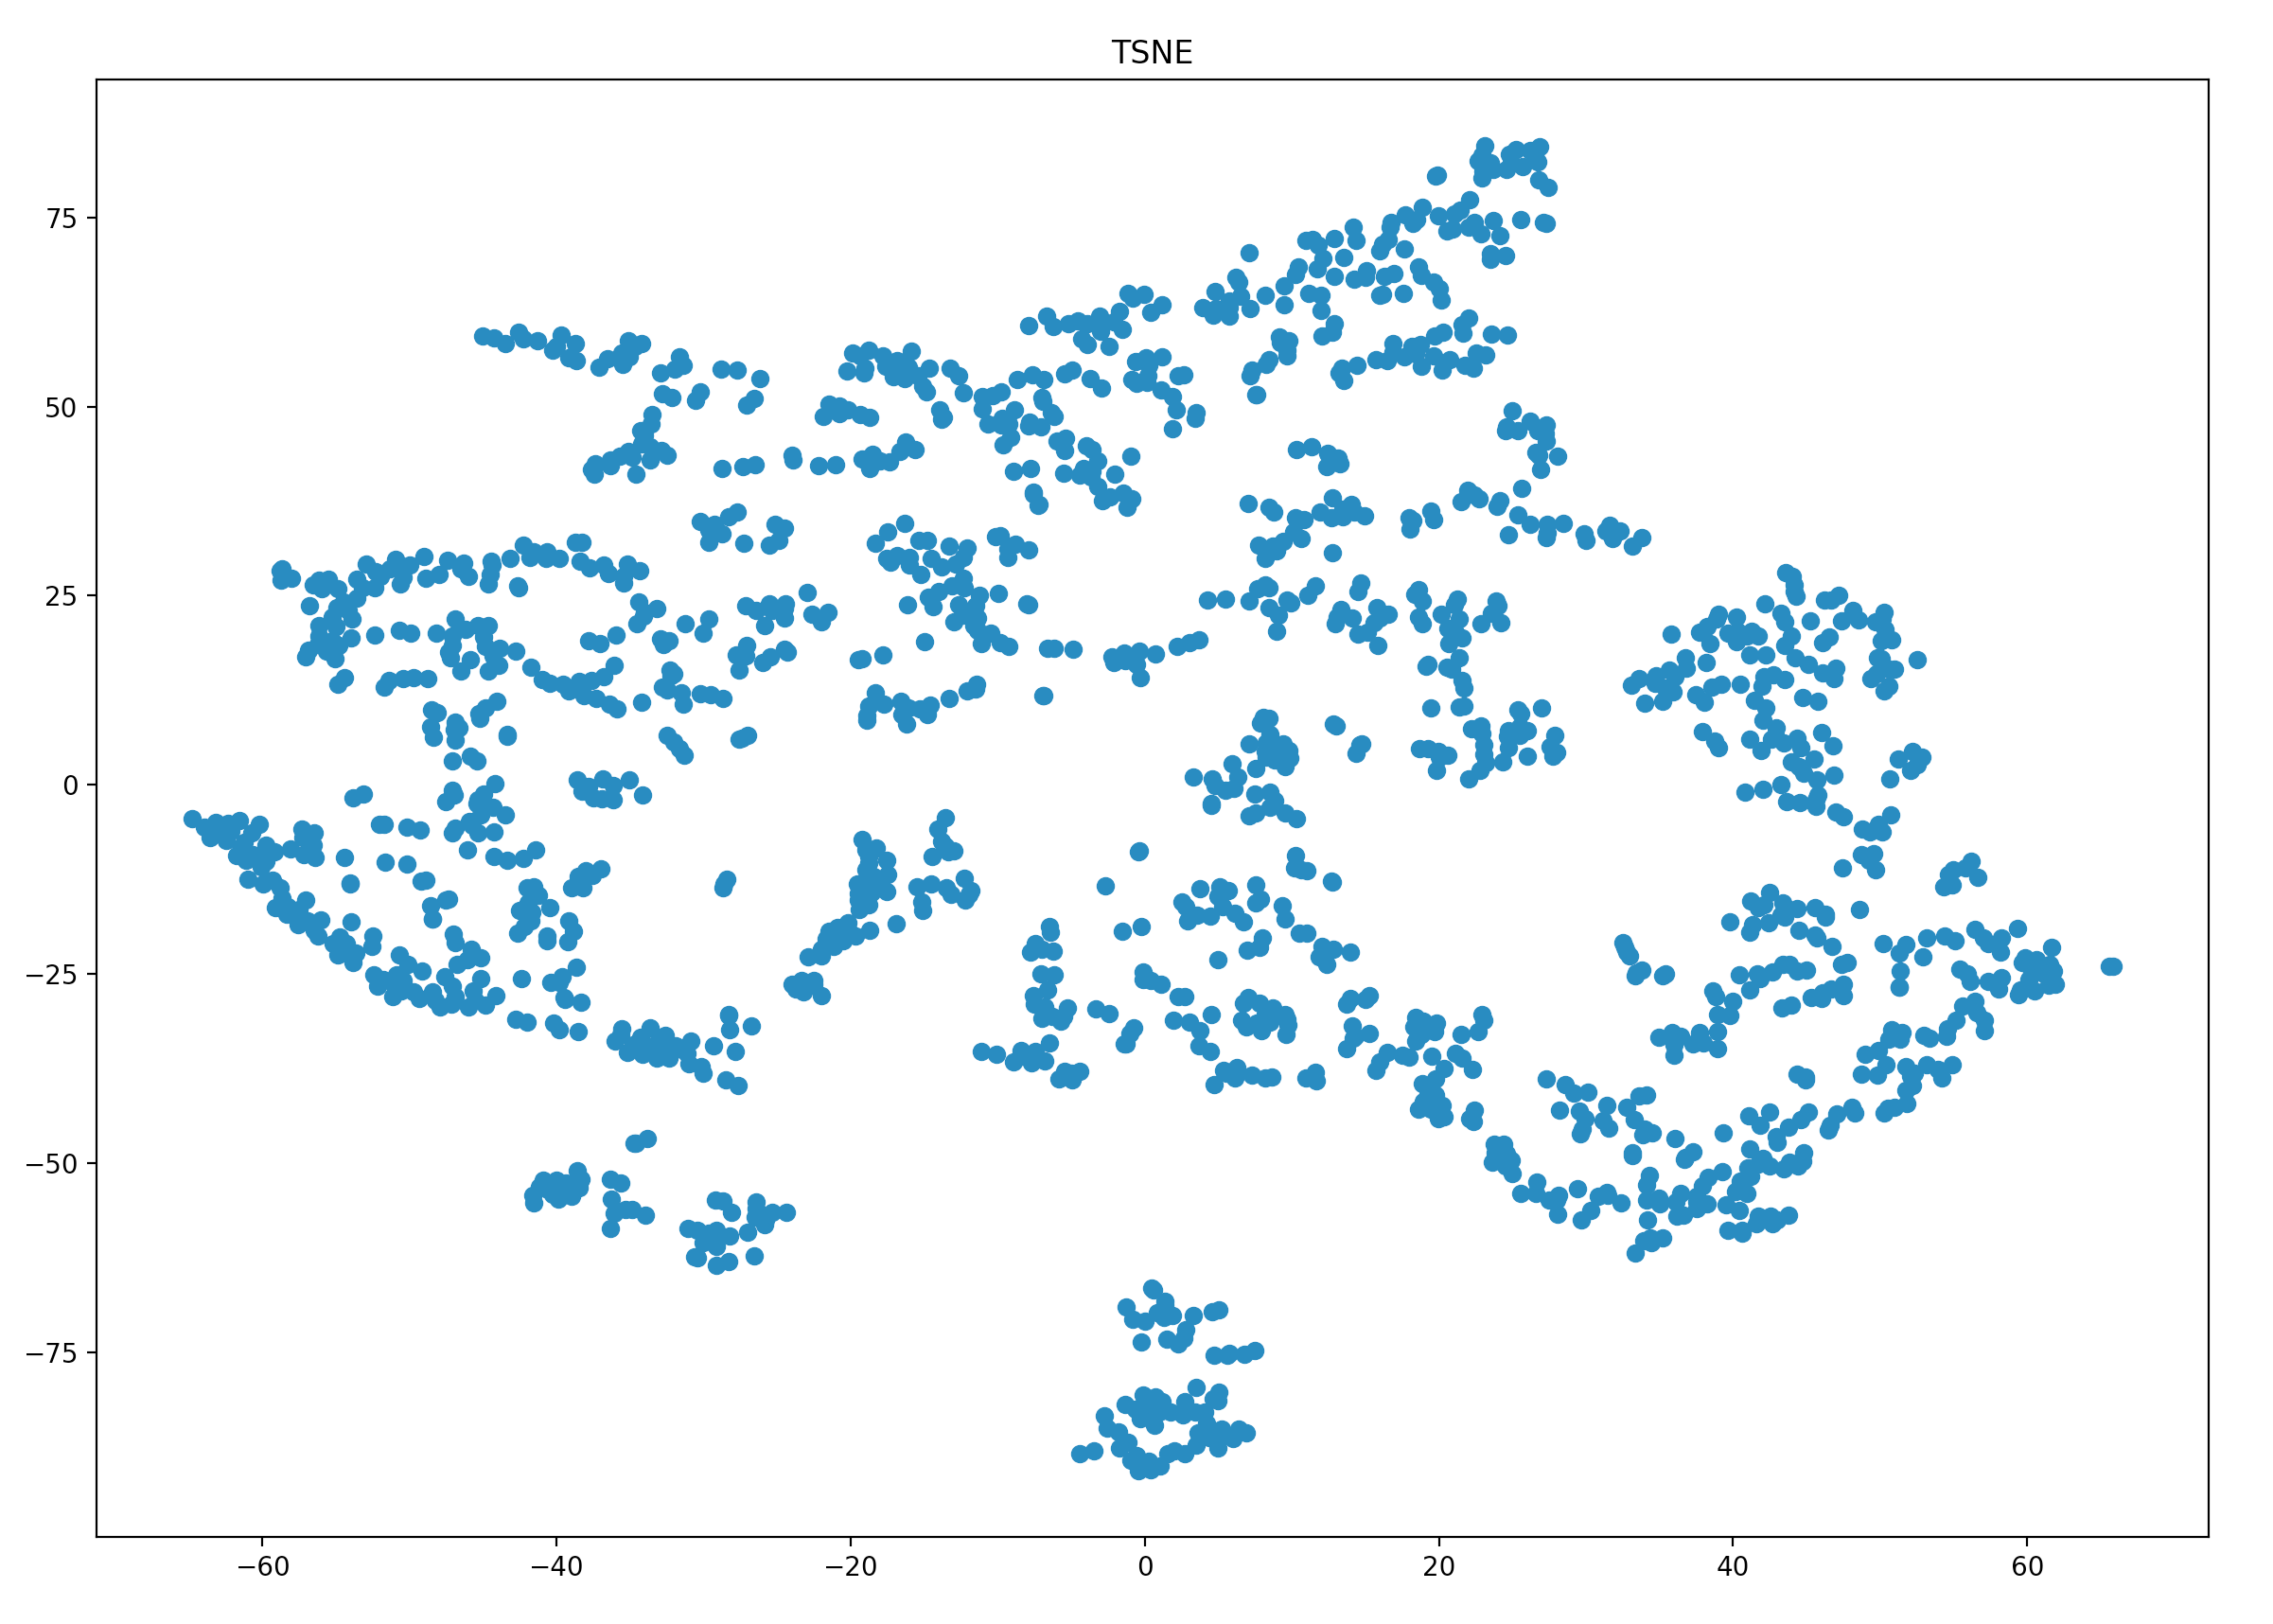
\includegraphics[width=0.9\textwidth]{./images/tsneParametersTest/perplexity/perp20-1hTSNE.png}
  % \caption{}
  % \label{figure:}
  \end{subfigure}%
  \begin{subfigure}{.5\textwidth}
    \centering
    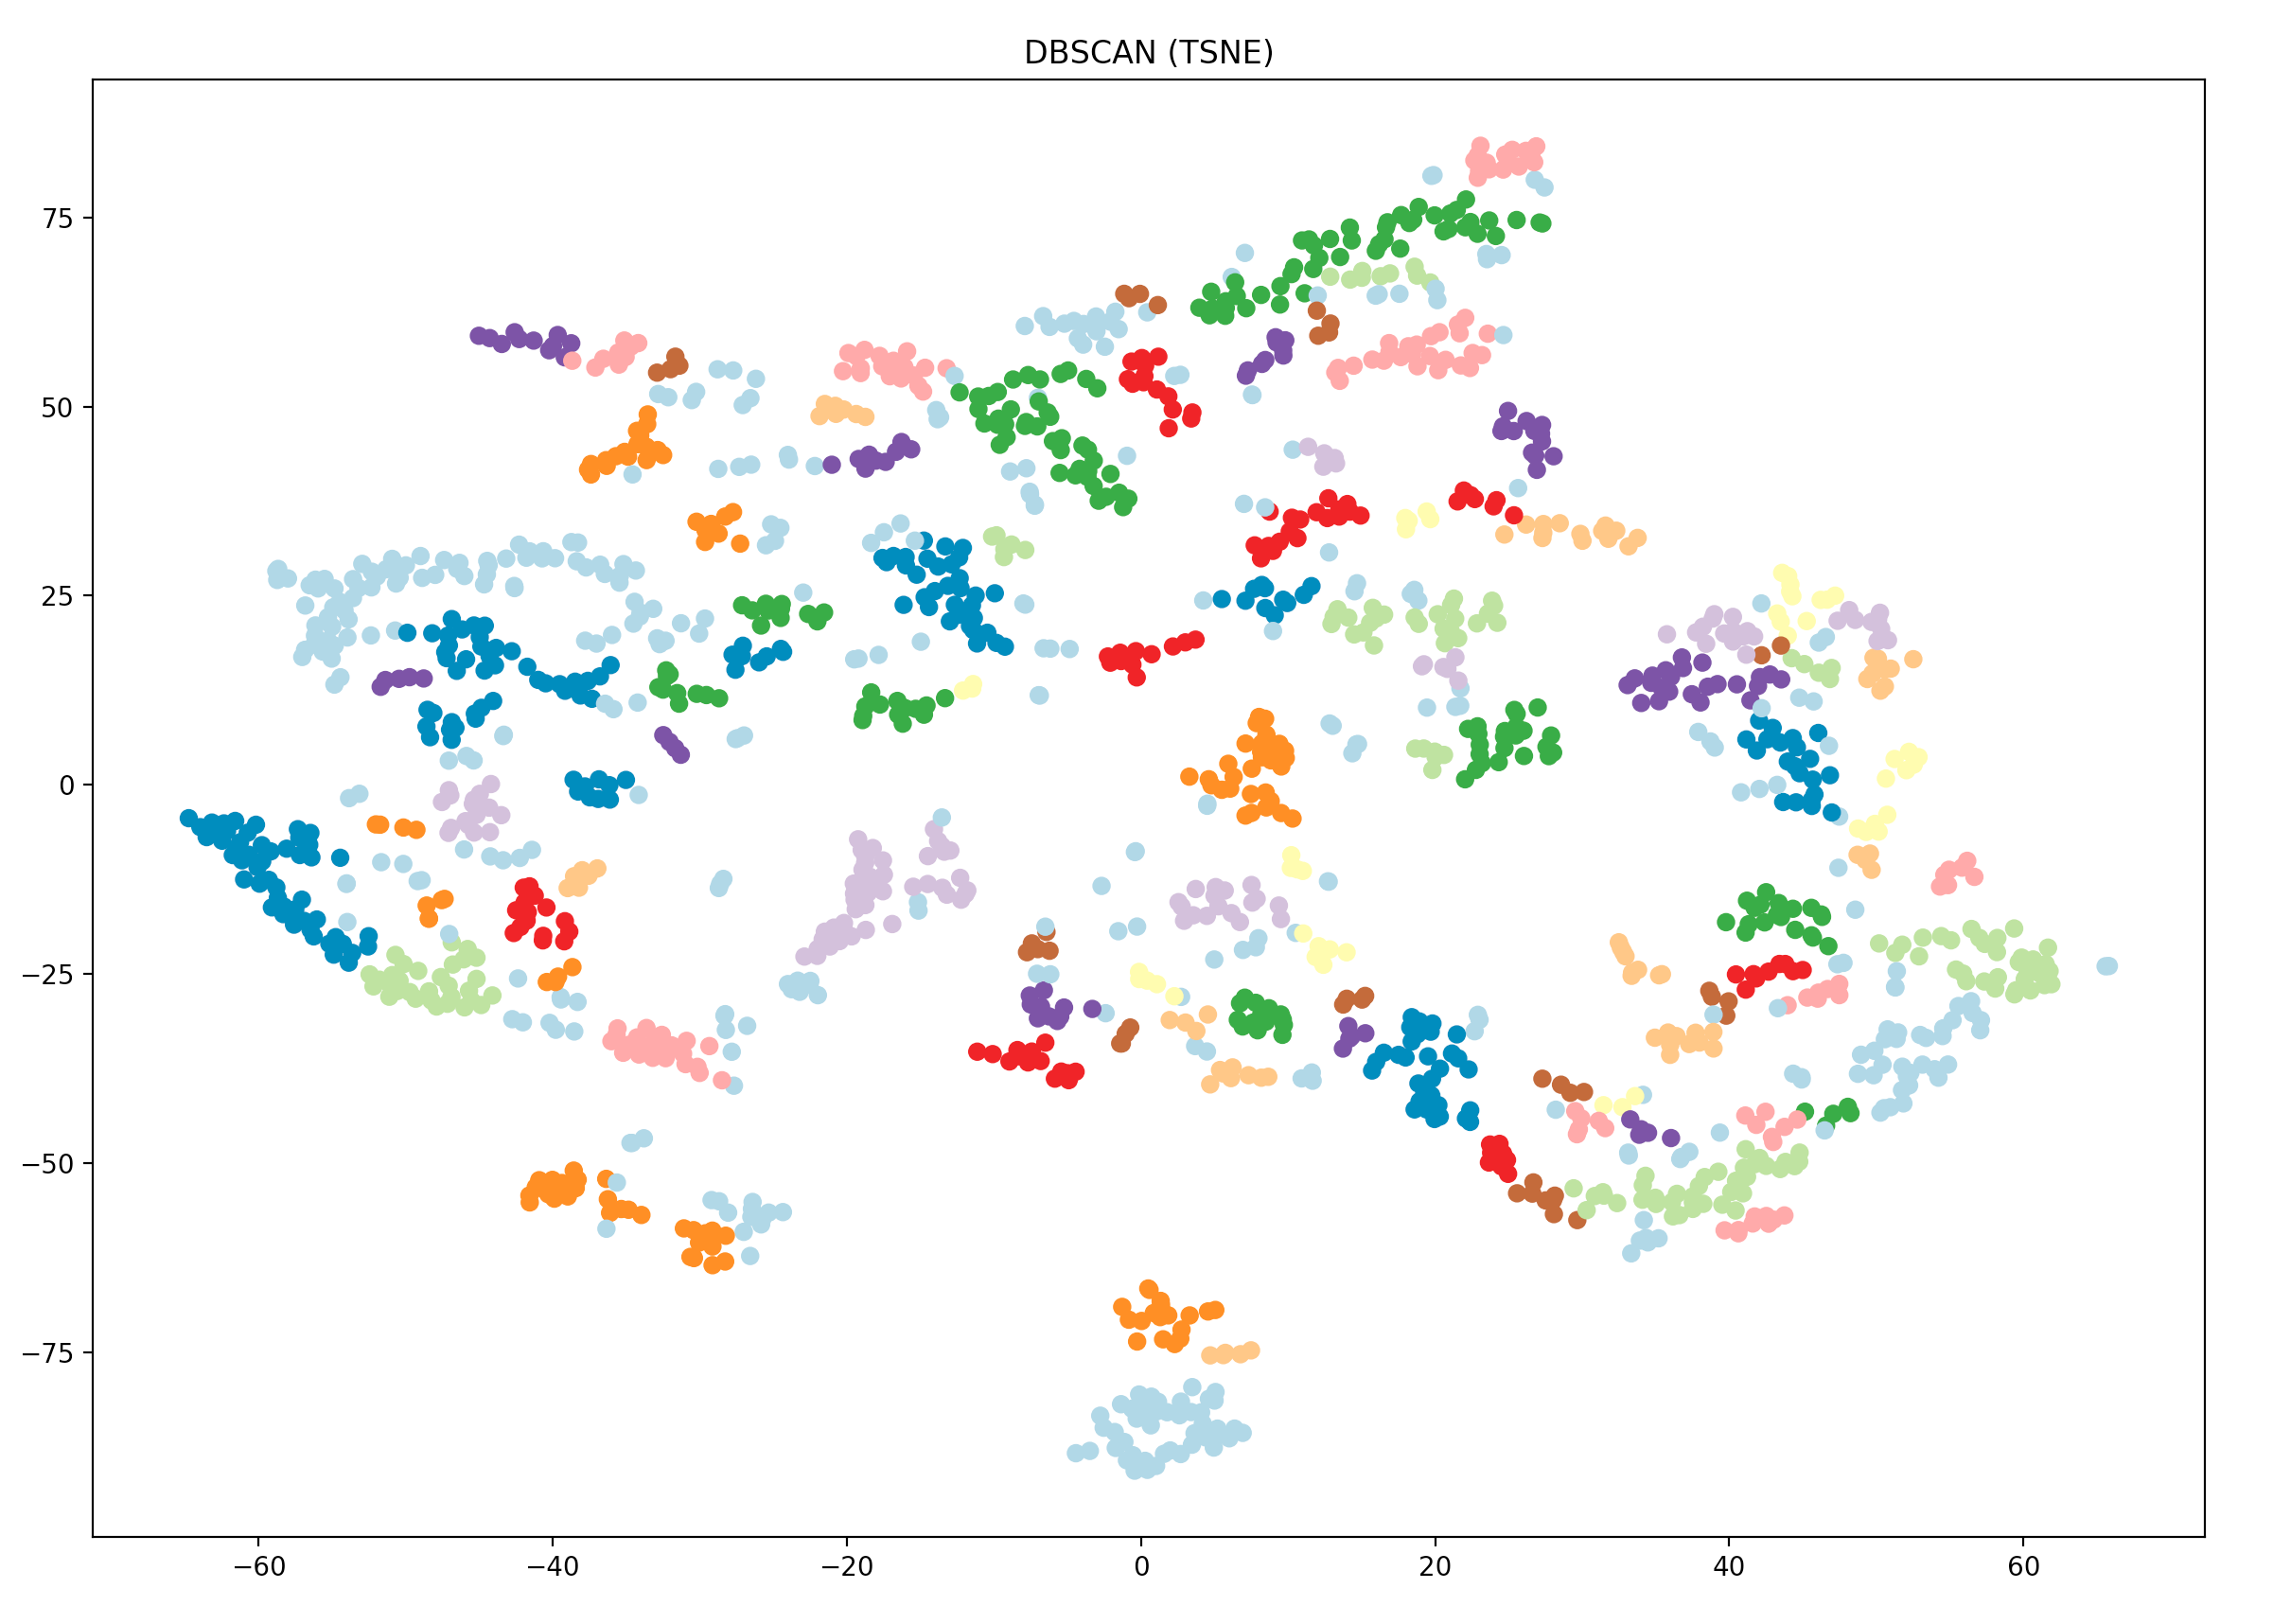
\includegraphics[width=0.9\textwidth]{./images/tsneParametersTest/perplexity/perp20-1hDBSCAN.png}
    % \caption{}
    % \label{figure:}
  \end{subfigure}
	\caption{\textbf{1h} data files, t-SNE calculated with the following parameters: \textbf{perplexity=20}, n\_iter=5000, learning\_rate=50}
  \label{figure:1hperp20TSNE}
\end{figure}

% -- 3h, perp 20 --
\begin{figure}[H]
  \centering
	\begin{subfigure}{.5\textwidth}
    \centering
    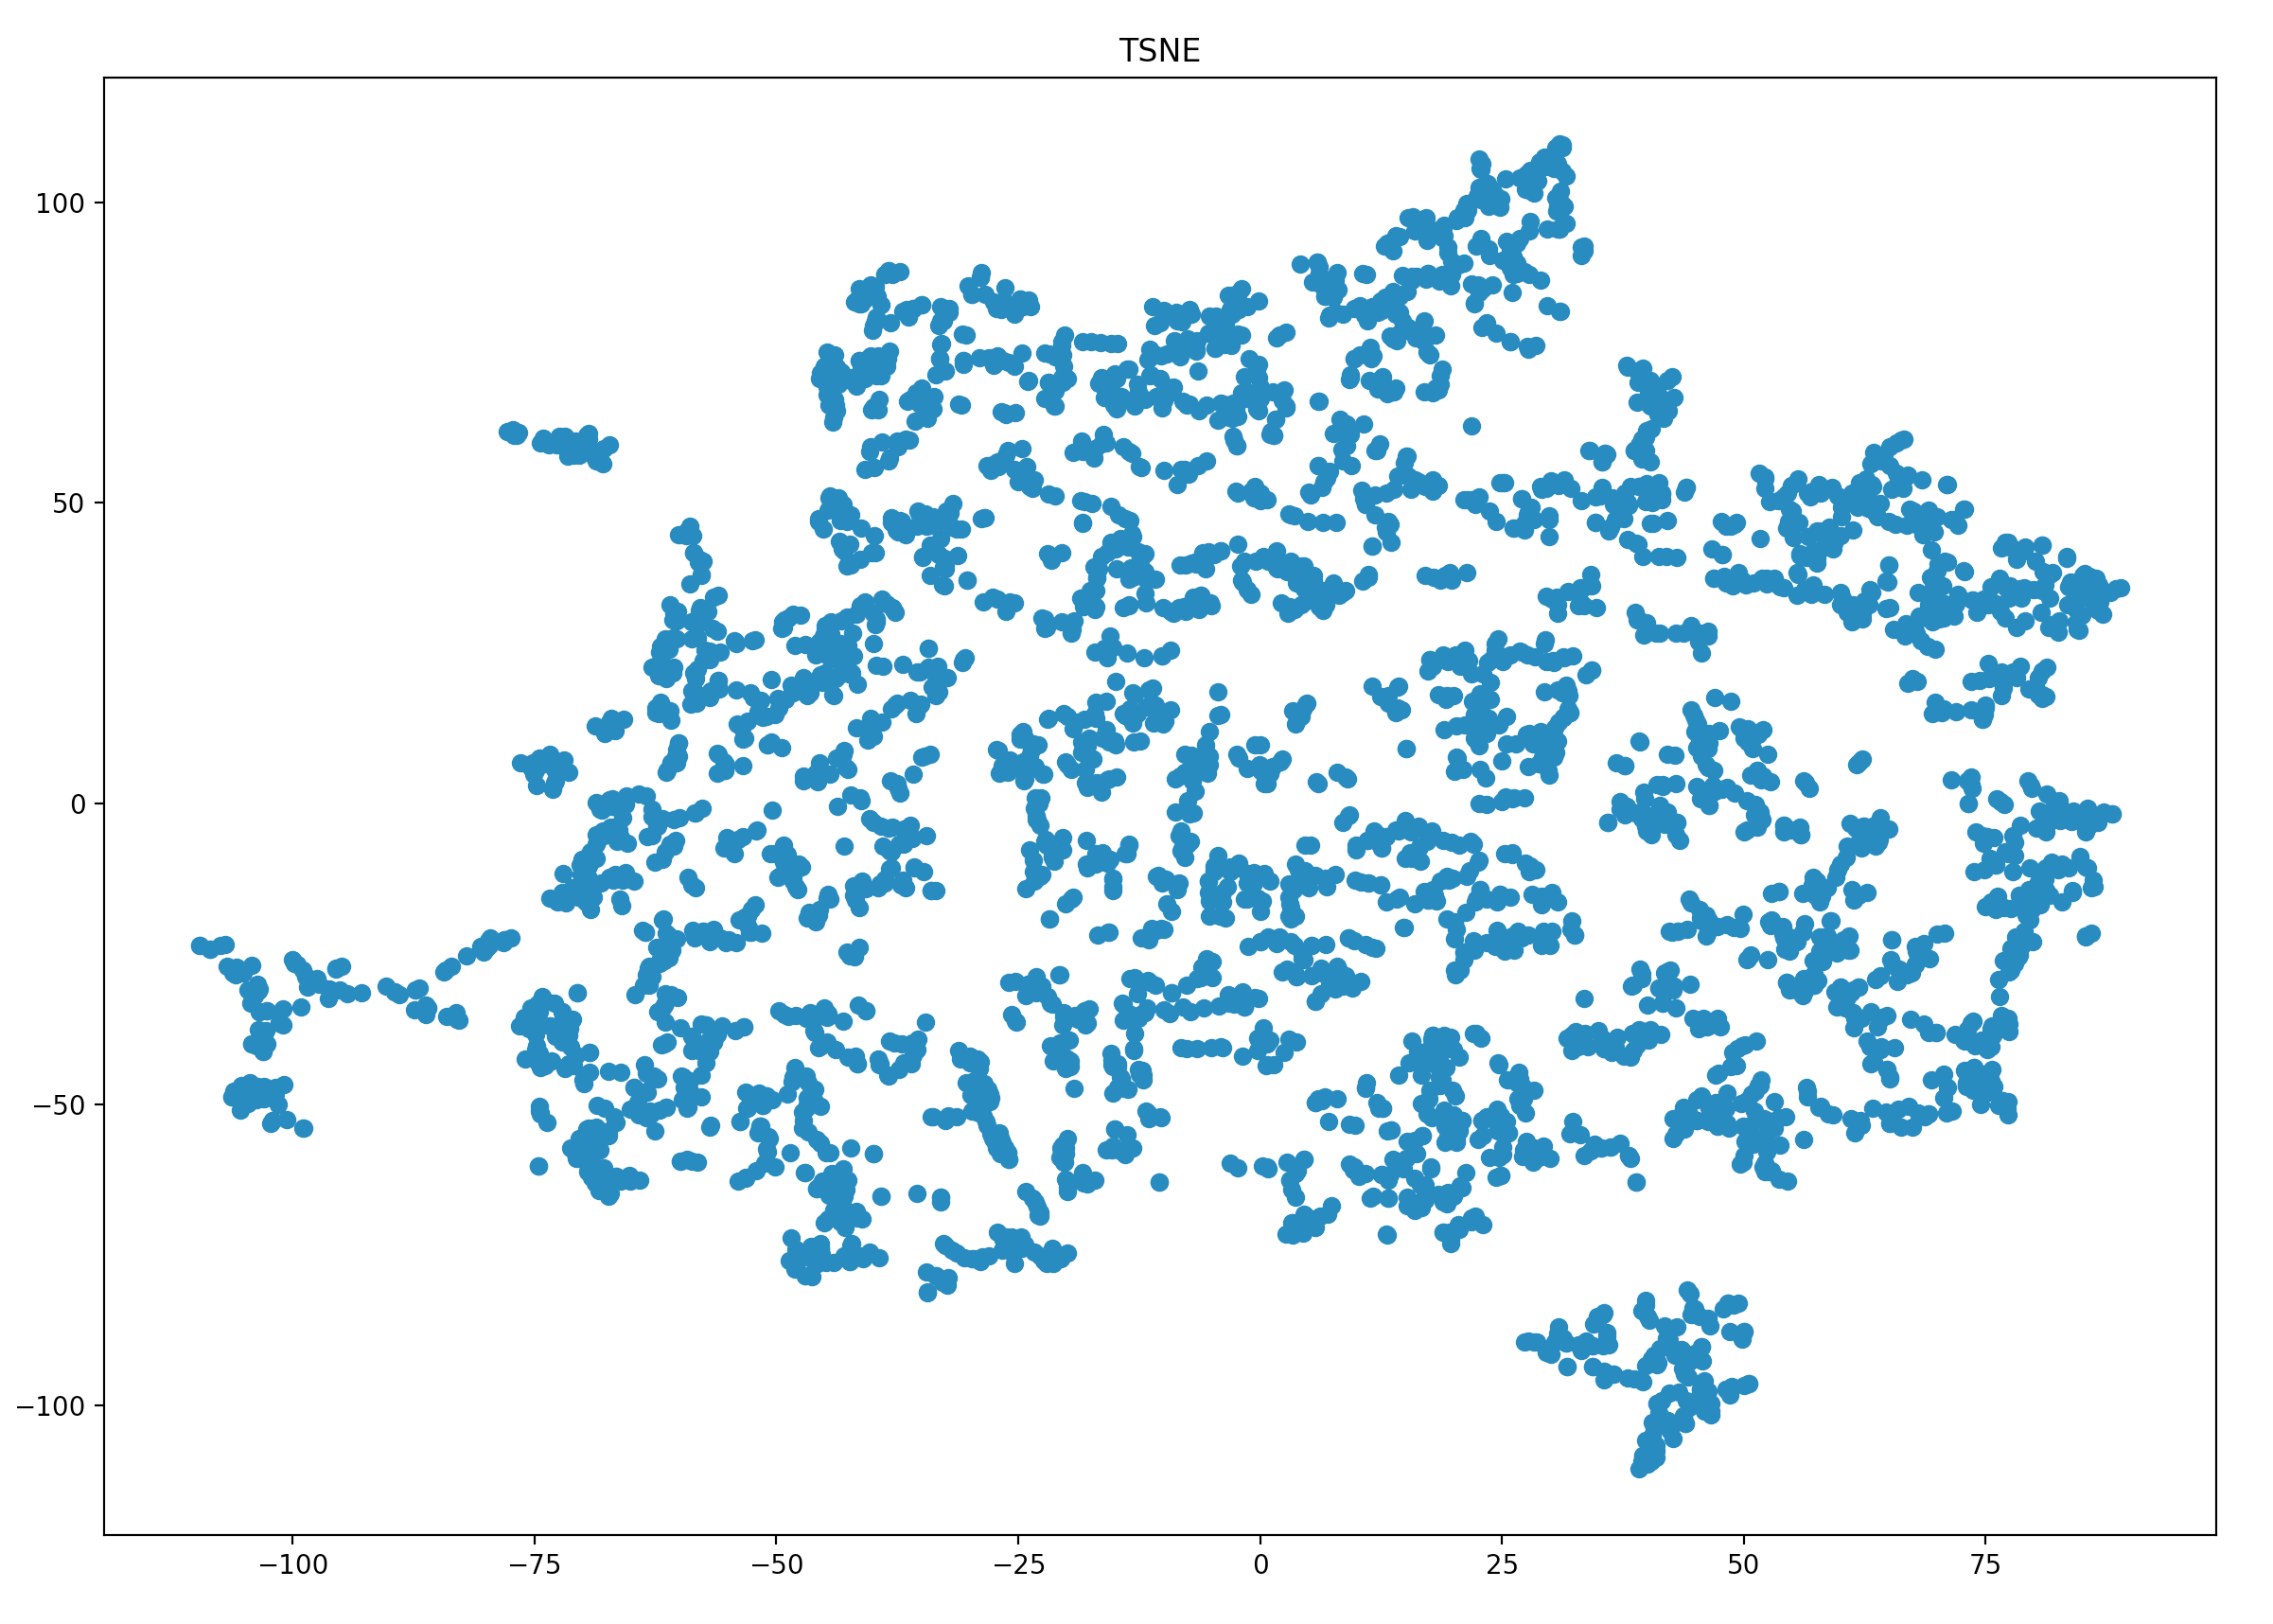
\includegraphics[width=0.9\textwidth]{./images/tsneParametersTest/perplexity/perp20-3hTSNE.png}
  % \caption{}
  % \label{figure:}
  \end{subfigure}%
  \begin{subfigure}{.5\textwidth}
    \centering
    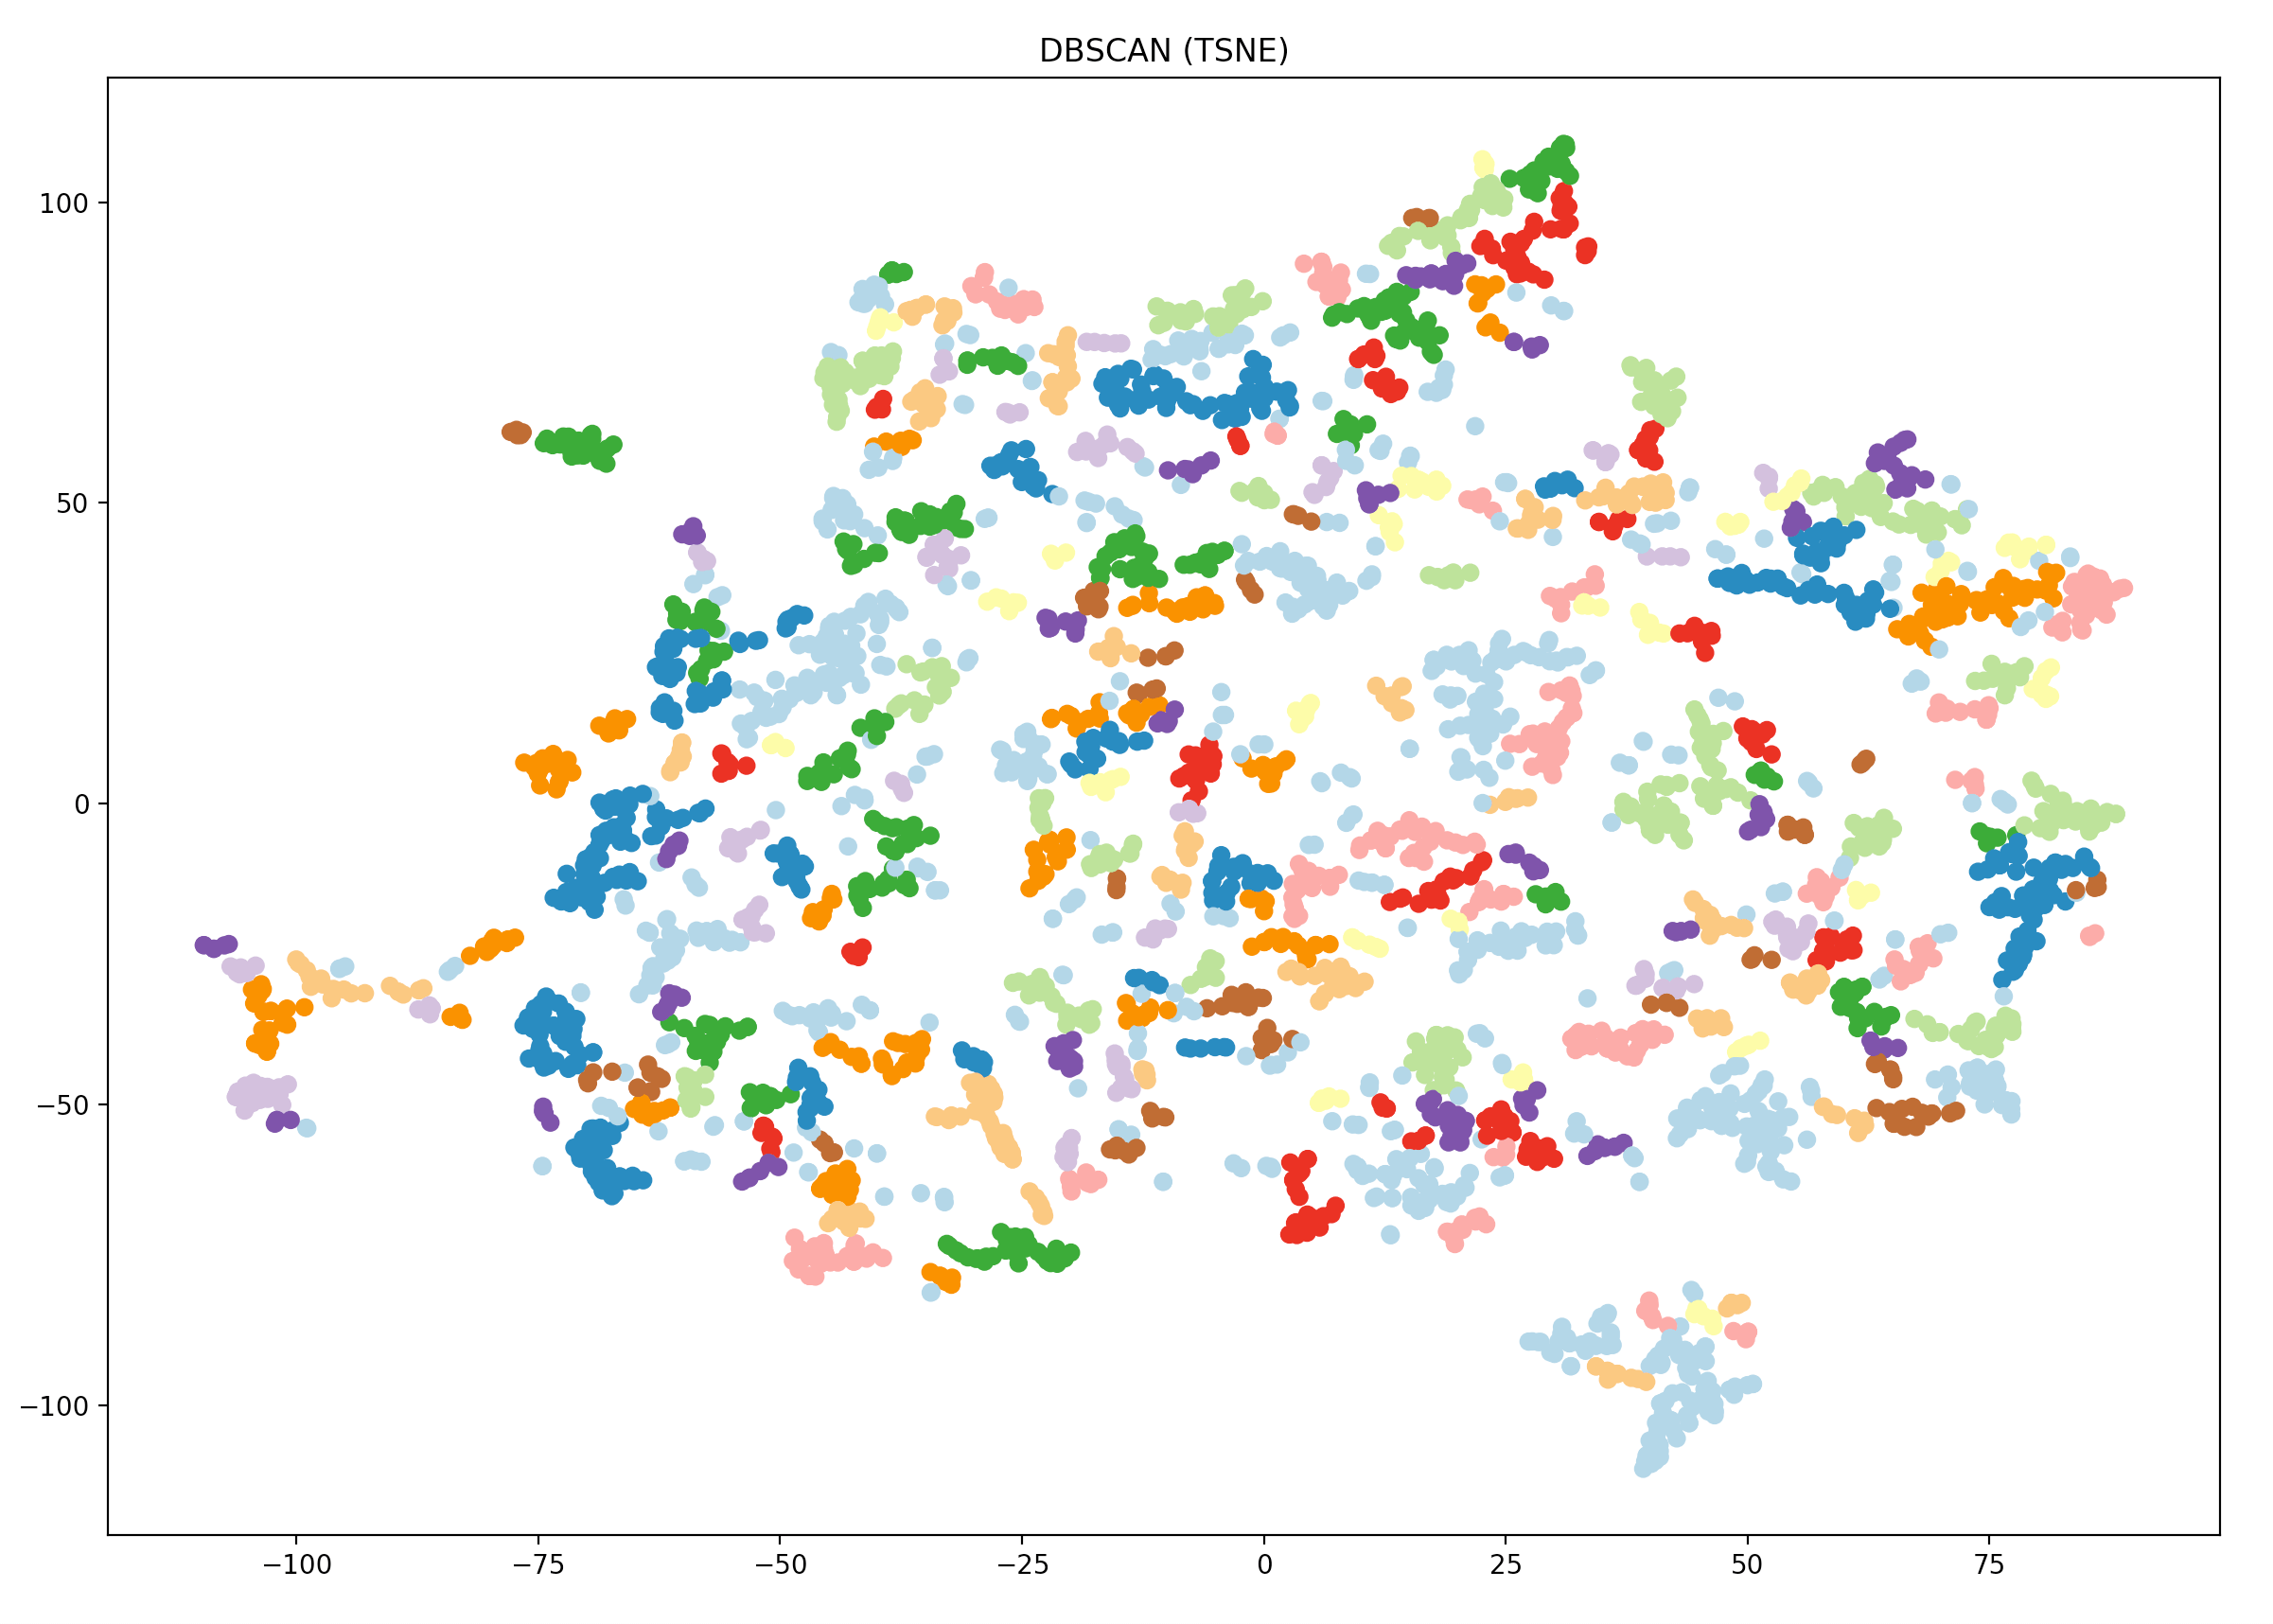
\includegraphics[width=0.9\textwidth]{./images/tsneParametersTest/perplexity/perp20-3hDBSCAN.png}
    % \caption{}
    % \label{figure:}
	\end{subfigure}
	\caption{\textbf{3h} data files, t-SNE calculated with the following parameters: \textbf{perplexity=20}, n\_iter=5000, learning\_rate=50}
  \label{figure:3hperp20TSNE}
\end{figure}



%------------------ PERPLEXITY 30: ------------------
\subsubsection{Perplexity = 30}
% -- 1h, perp 30 --
\begin{figure}[H]
  \centering
  \begin{subfigure}{.5\textwidth}
    \centering
    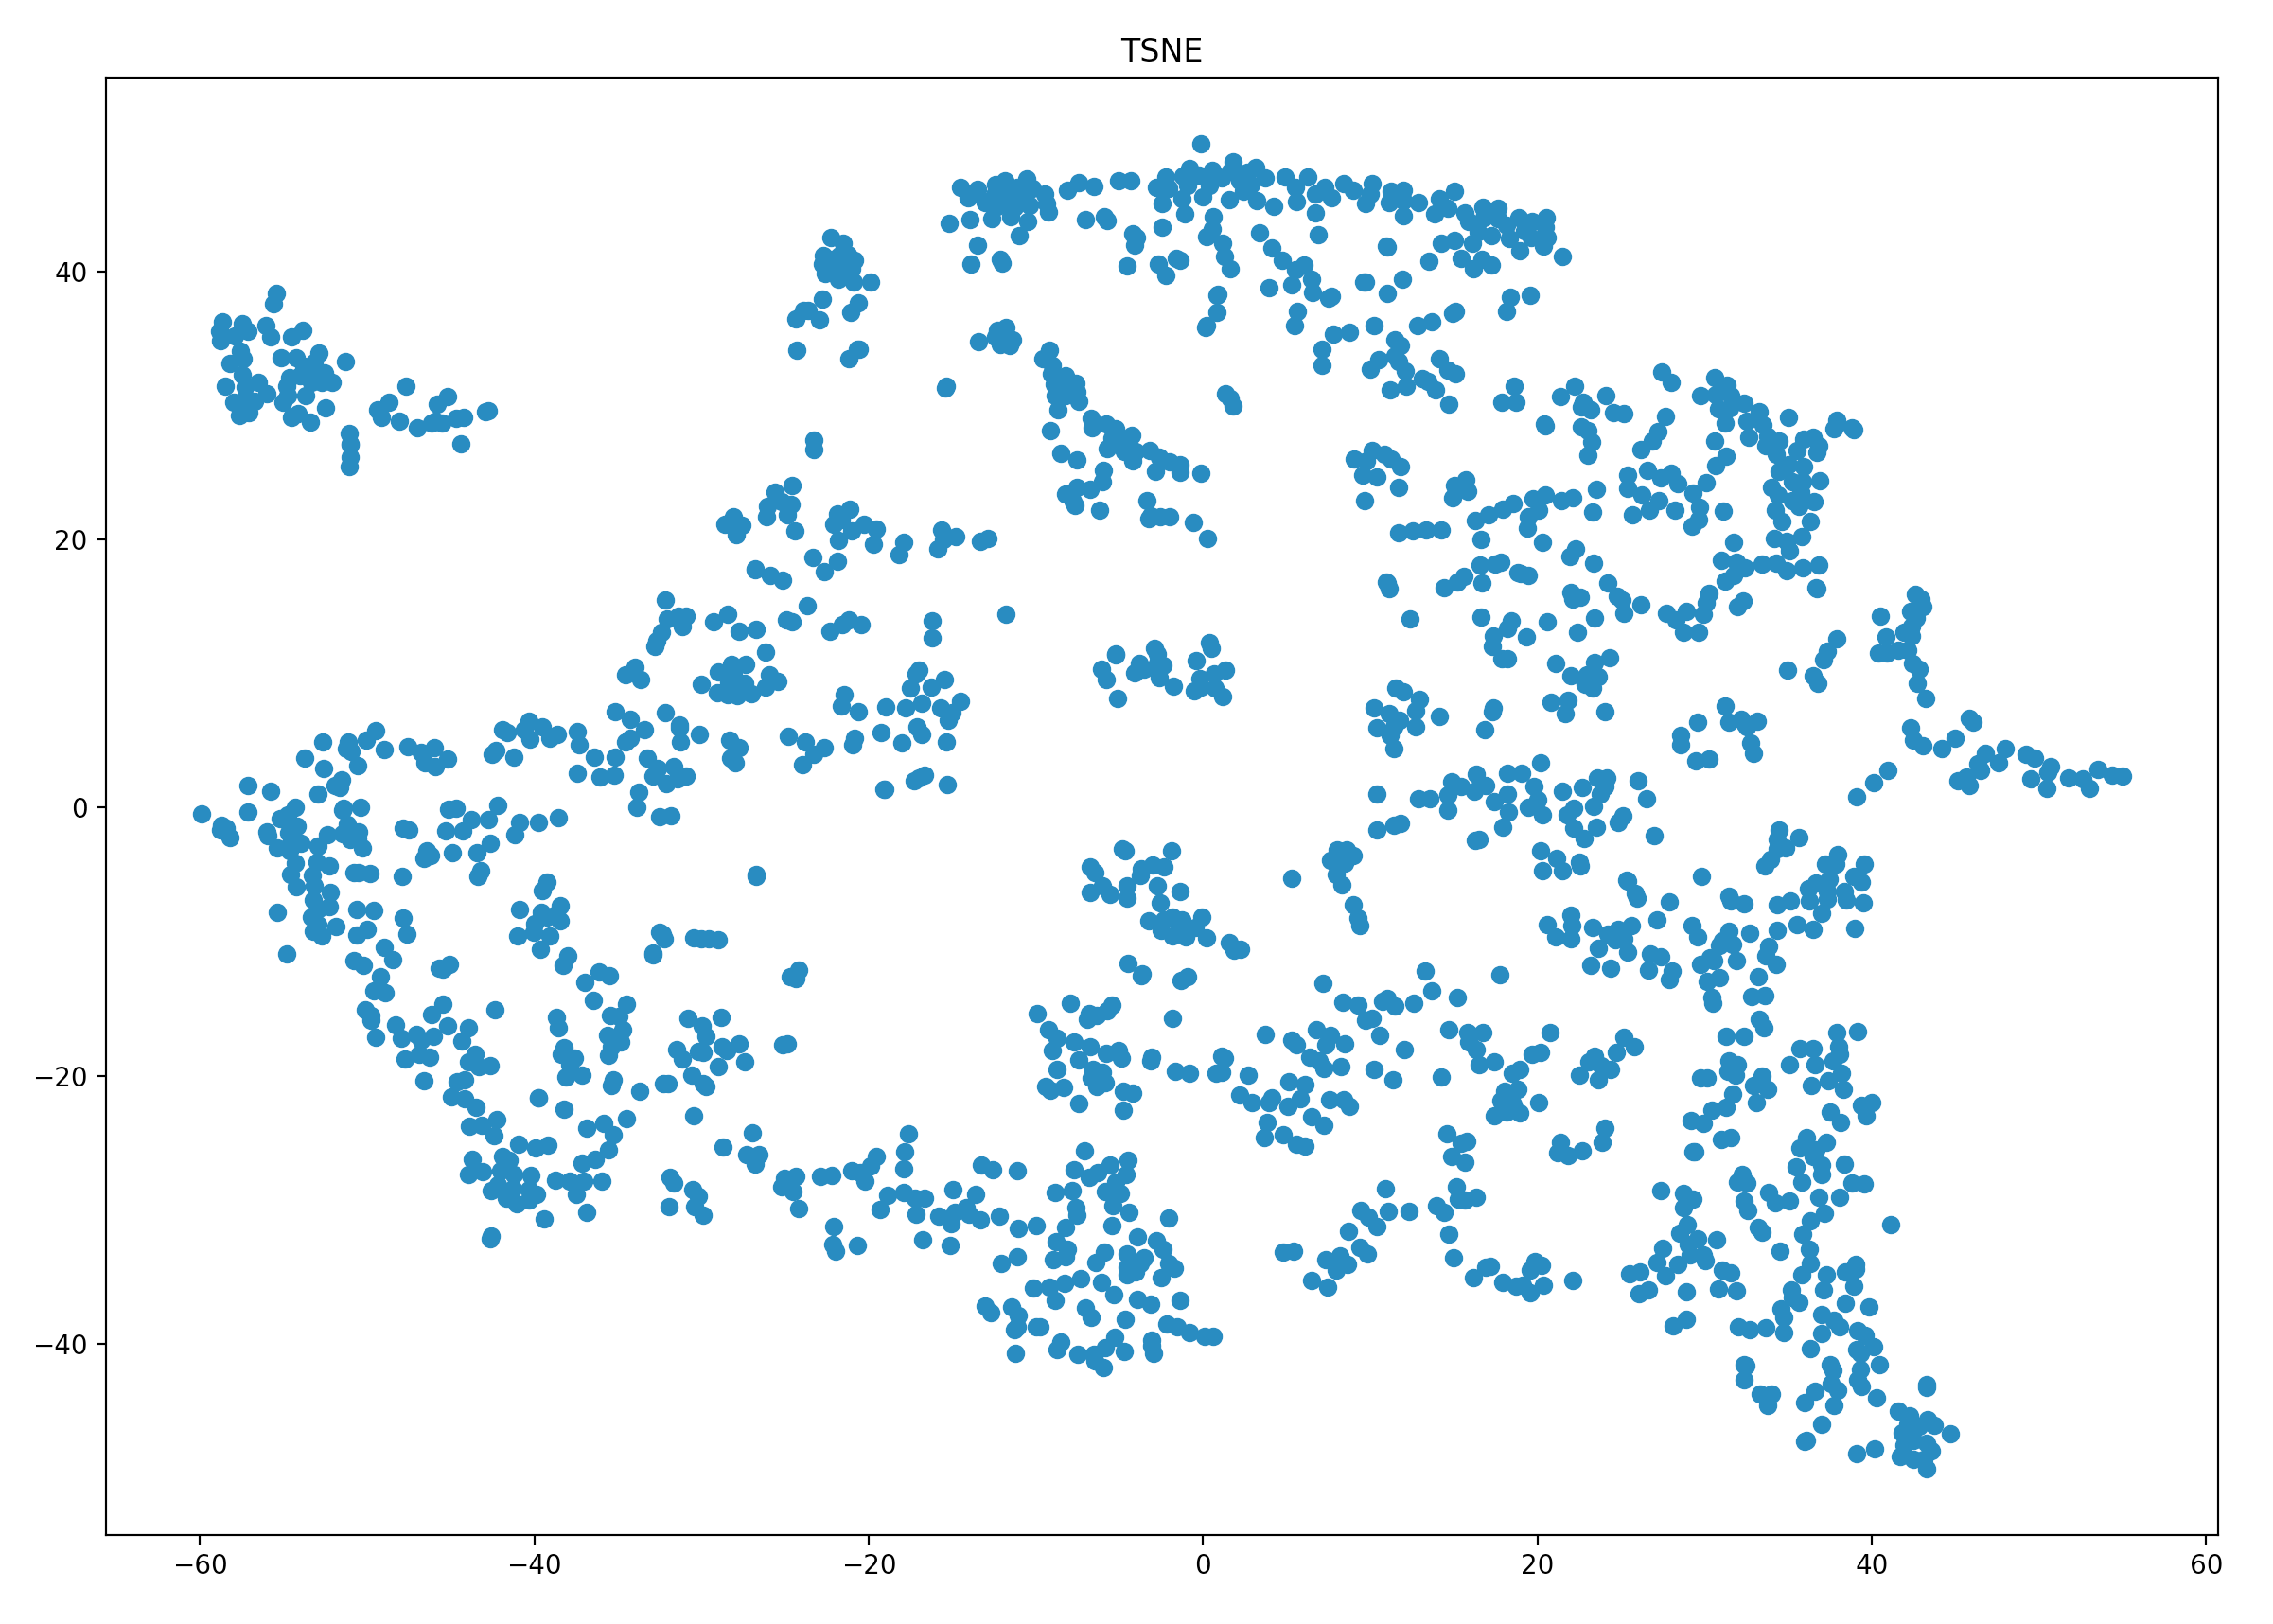
\includegraphics[width=0.9\textwidth]{./images/tsneParametersTest/perplexity/perp30-1hTSNE.png}
  % \caption{}
  % \label{figure:}
  \end{subfigure}%
  \begin{subfigure}{.5\textwidth}
    \centering
    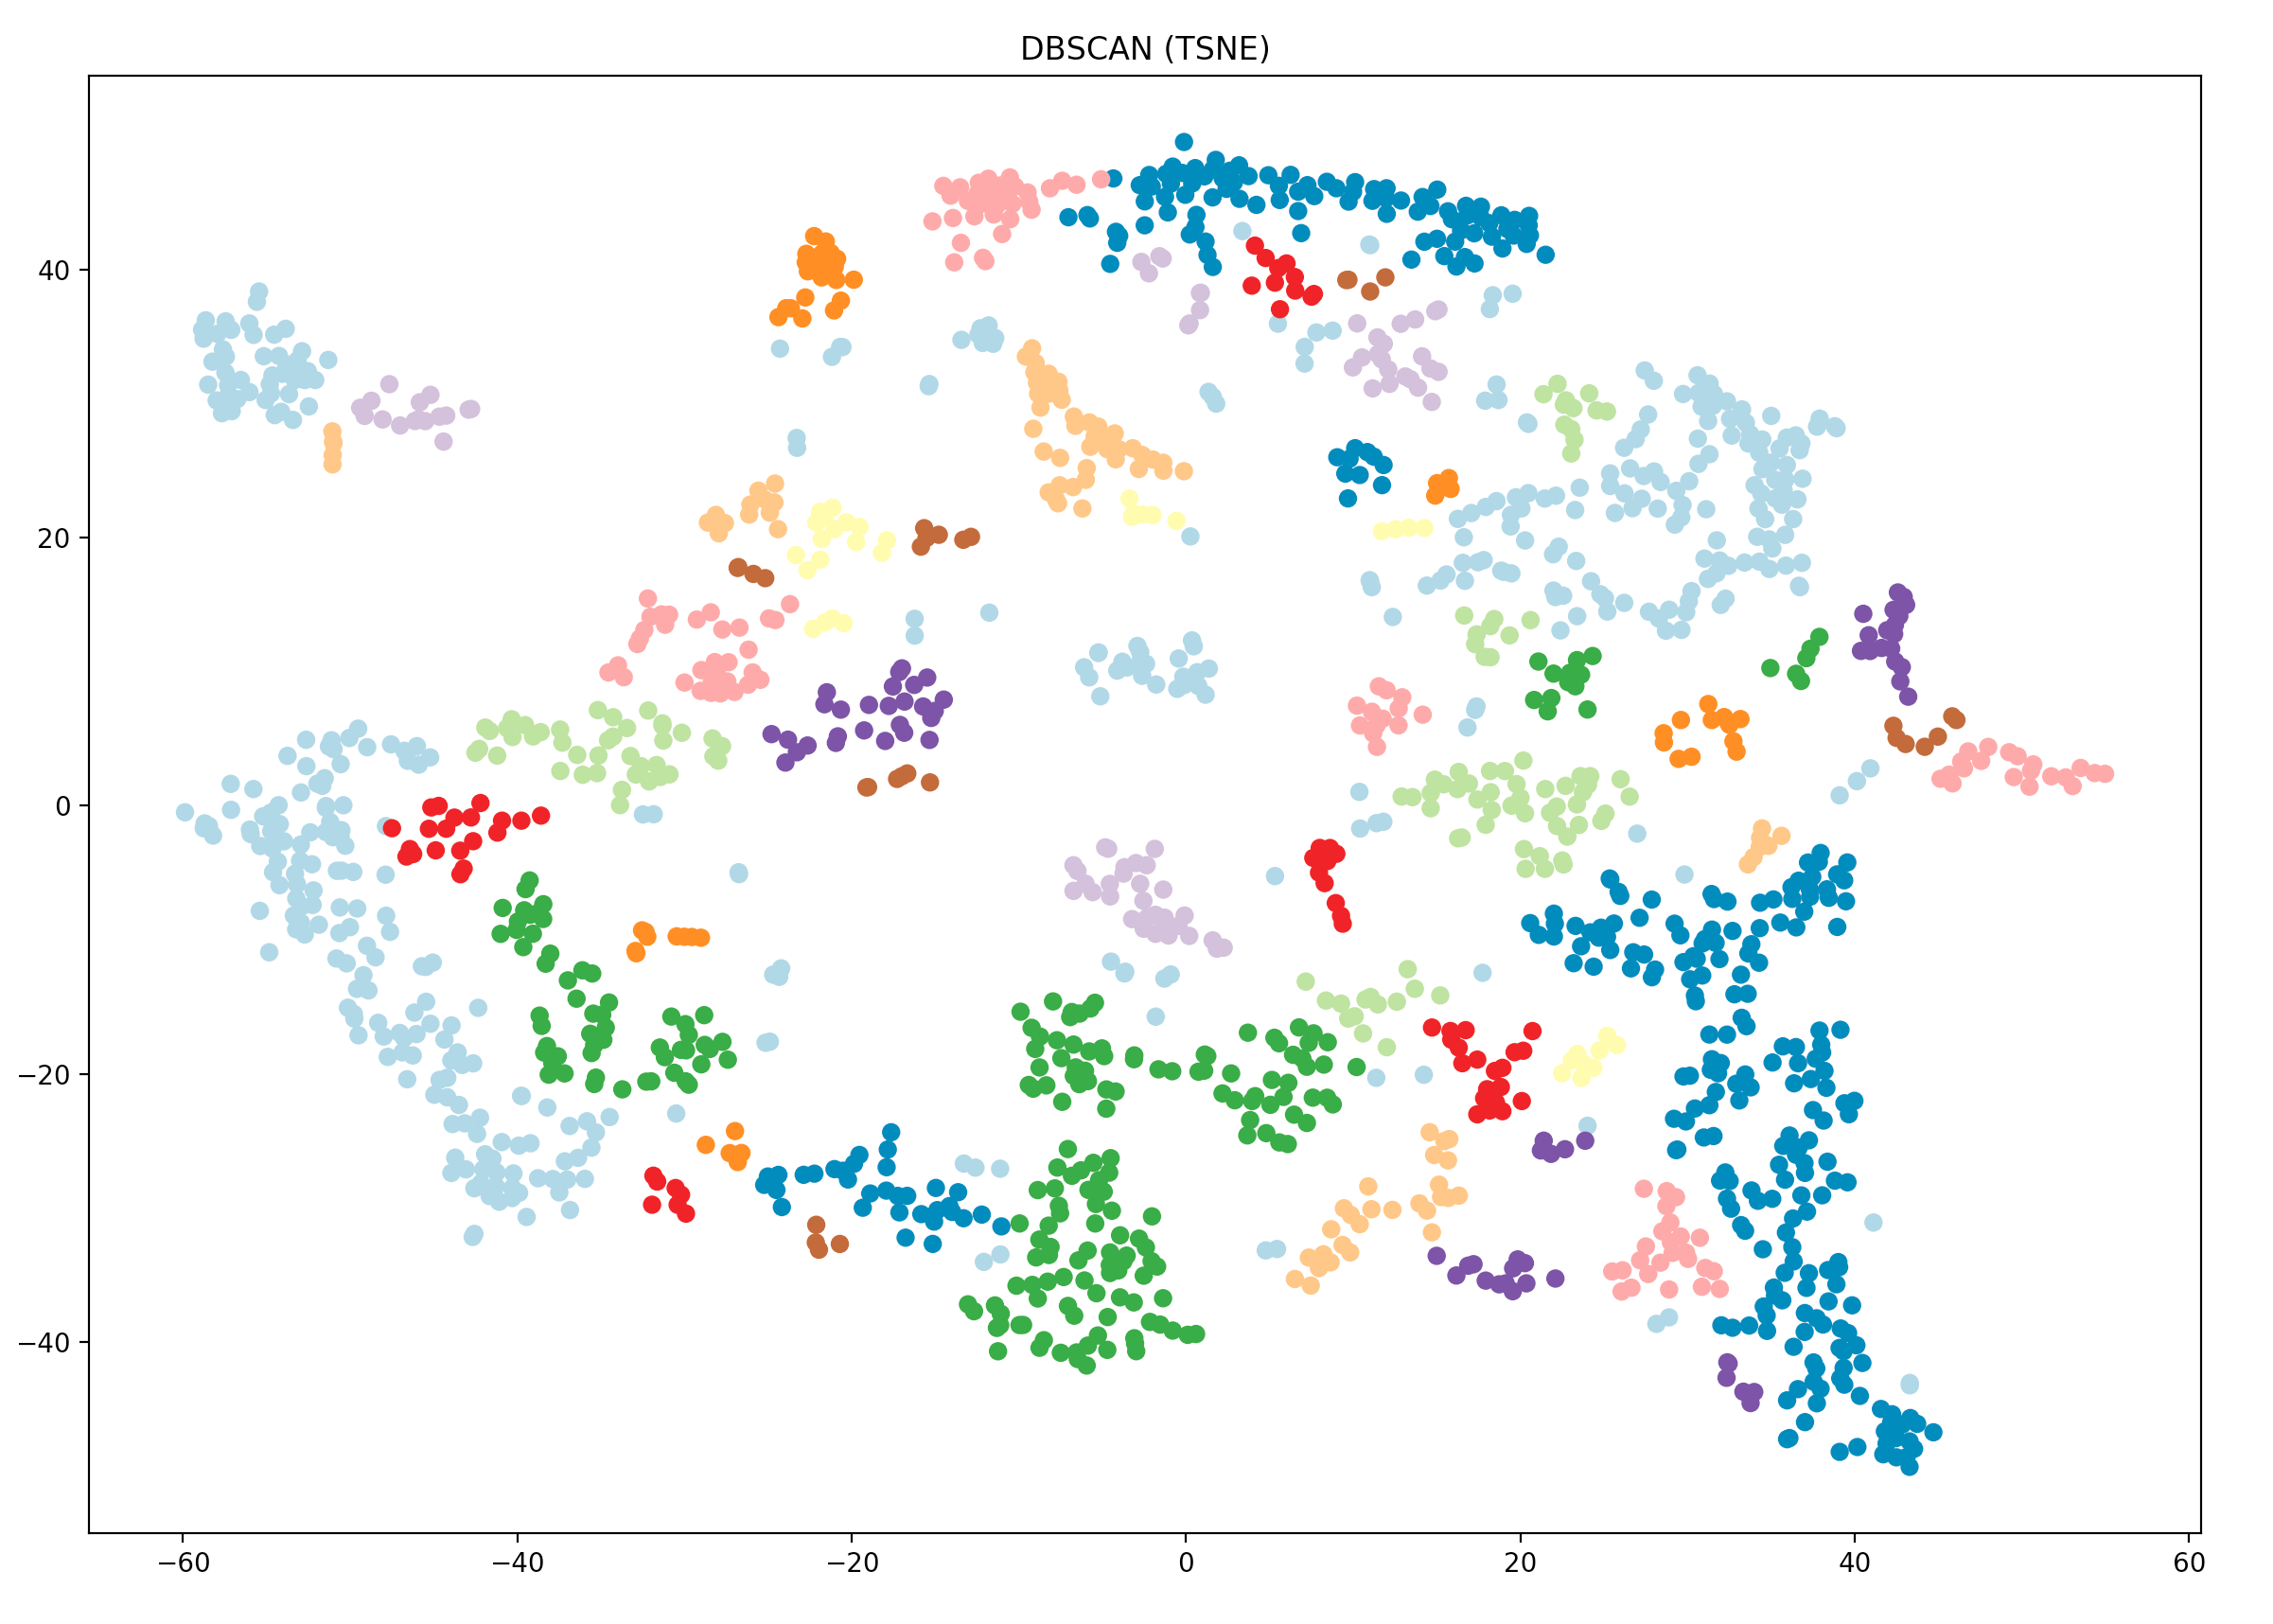
\includegraphics[width=0.9\textwidth]{./images/tsneParametersTest/perplexity/perp30-1hDBSCAN.png}
    % \caption{}
    % \label{figure:}
  \end{subfigure}
	\caption{\textbf{1h} data files, t-SNE calculated with the following parameters: \textbf{perplexity=30}, n\_iter=5000, learning\_rate=50}
  \label{figure:1hperp30TSNE}
\end{figure}

% -- 3h, perp 30 --
\begin{figure}[H]
  \centering
	\begin{subfigure}{.5\textwidth}
    \centering
    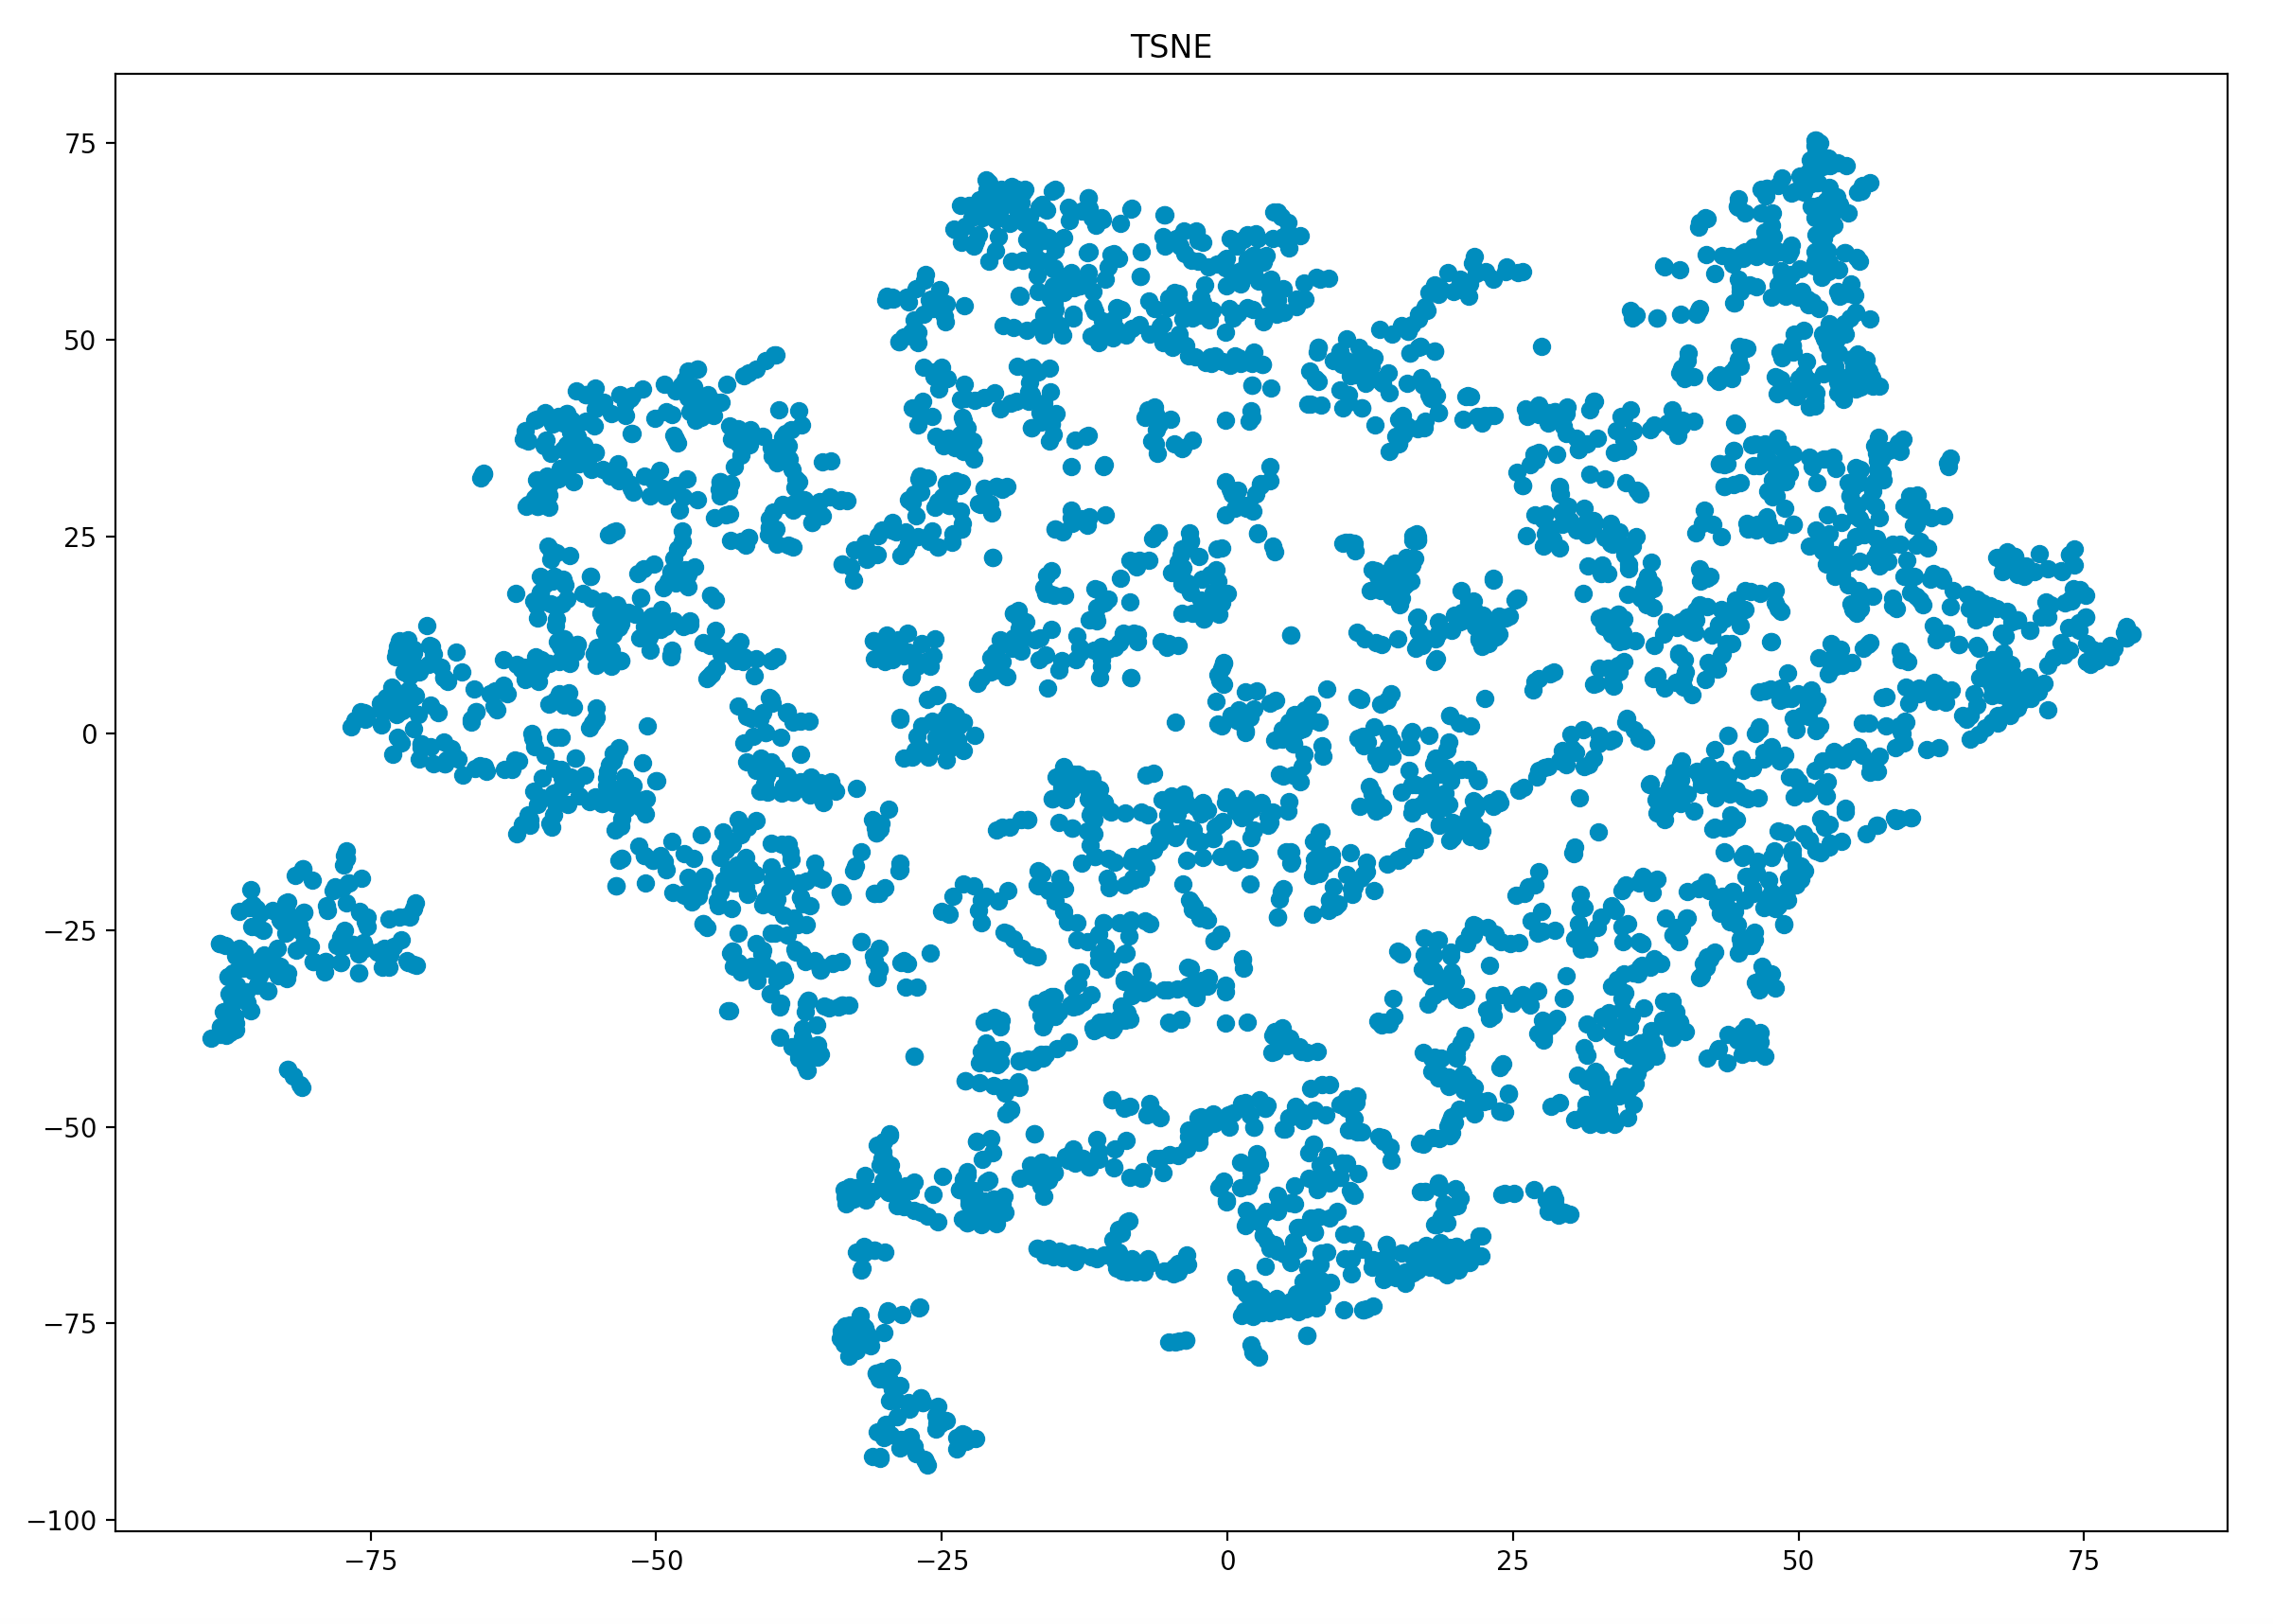
\includegraphics[width=0.9\textwidth]{./images/tsneParametersTest/perplexity/perp30-3hTSNE.png}
  % \caption{}
  % \label{figure:}
  \end{subfigure}%
  \begin{subfigure}{.5\textwidth}
    \centering
    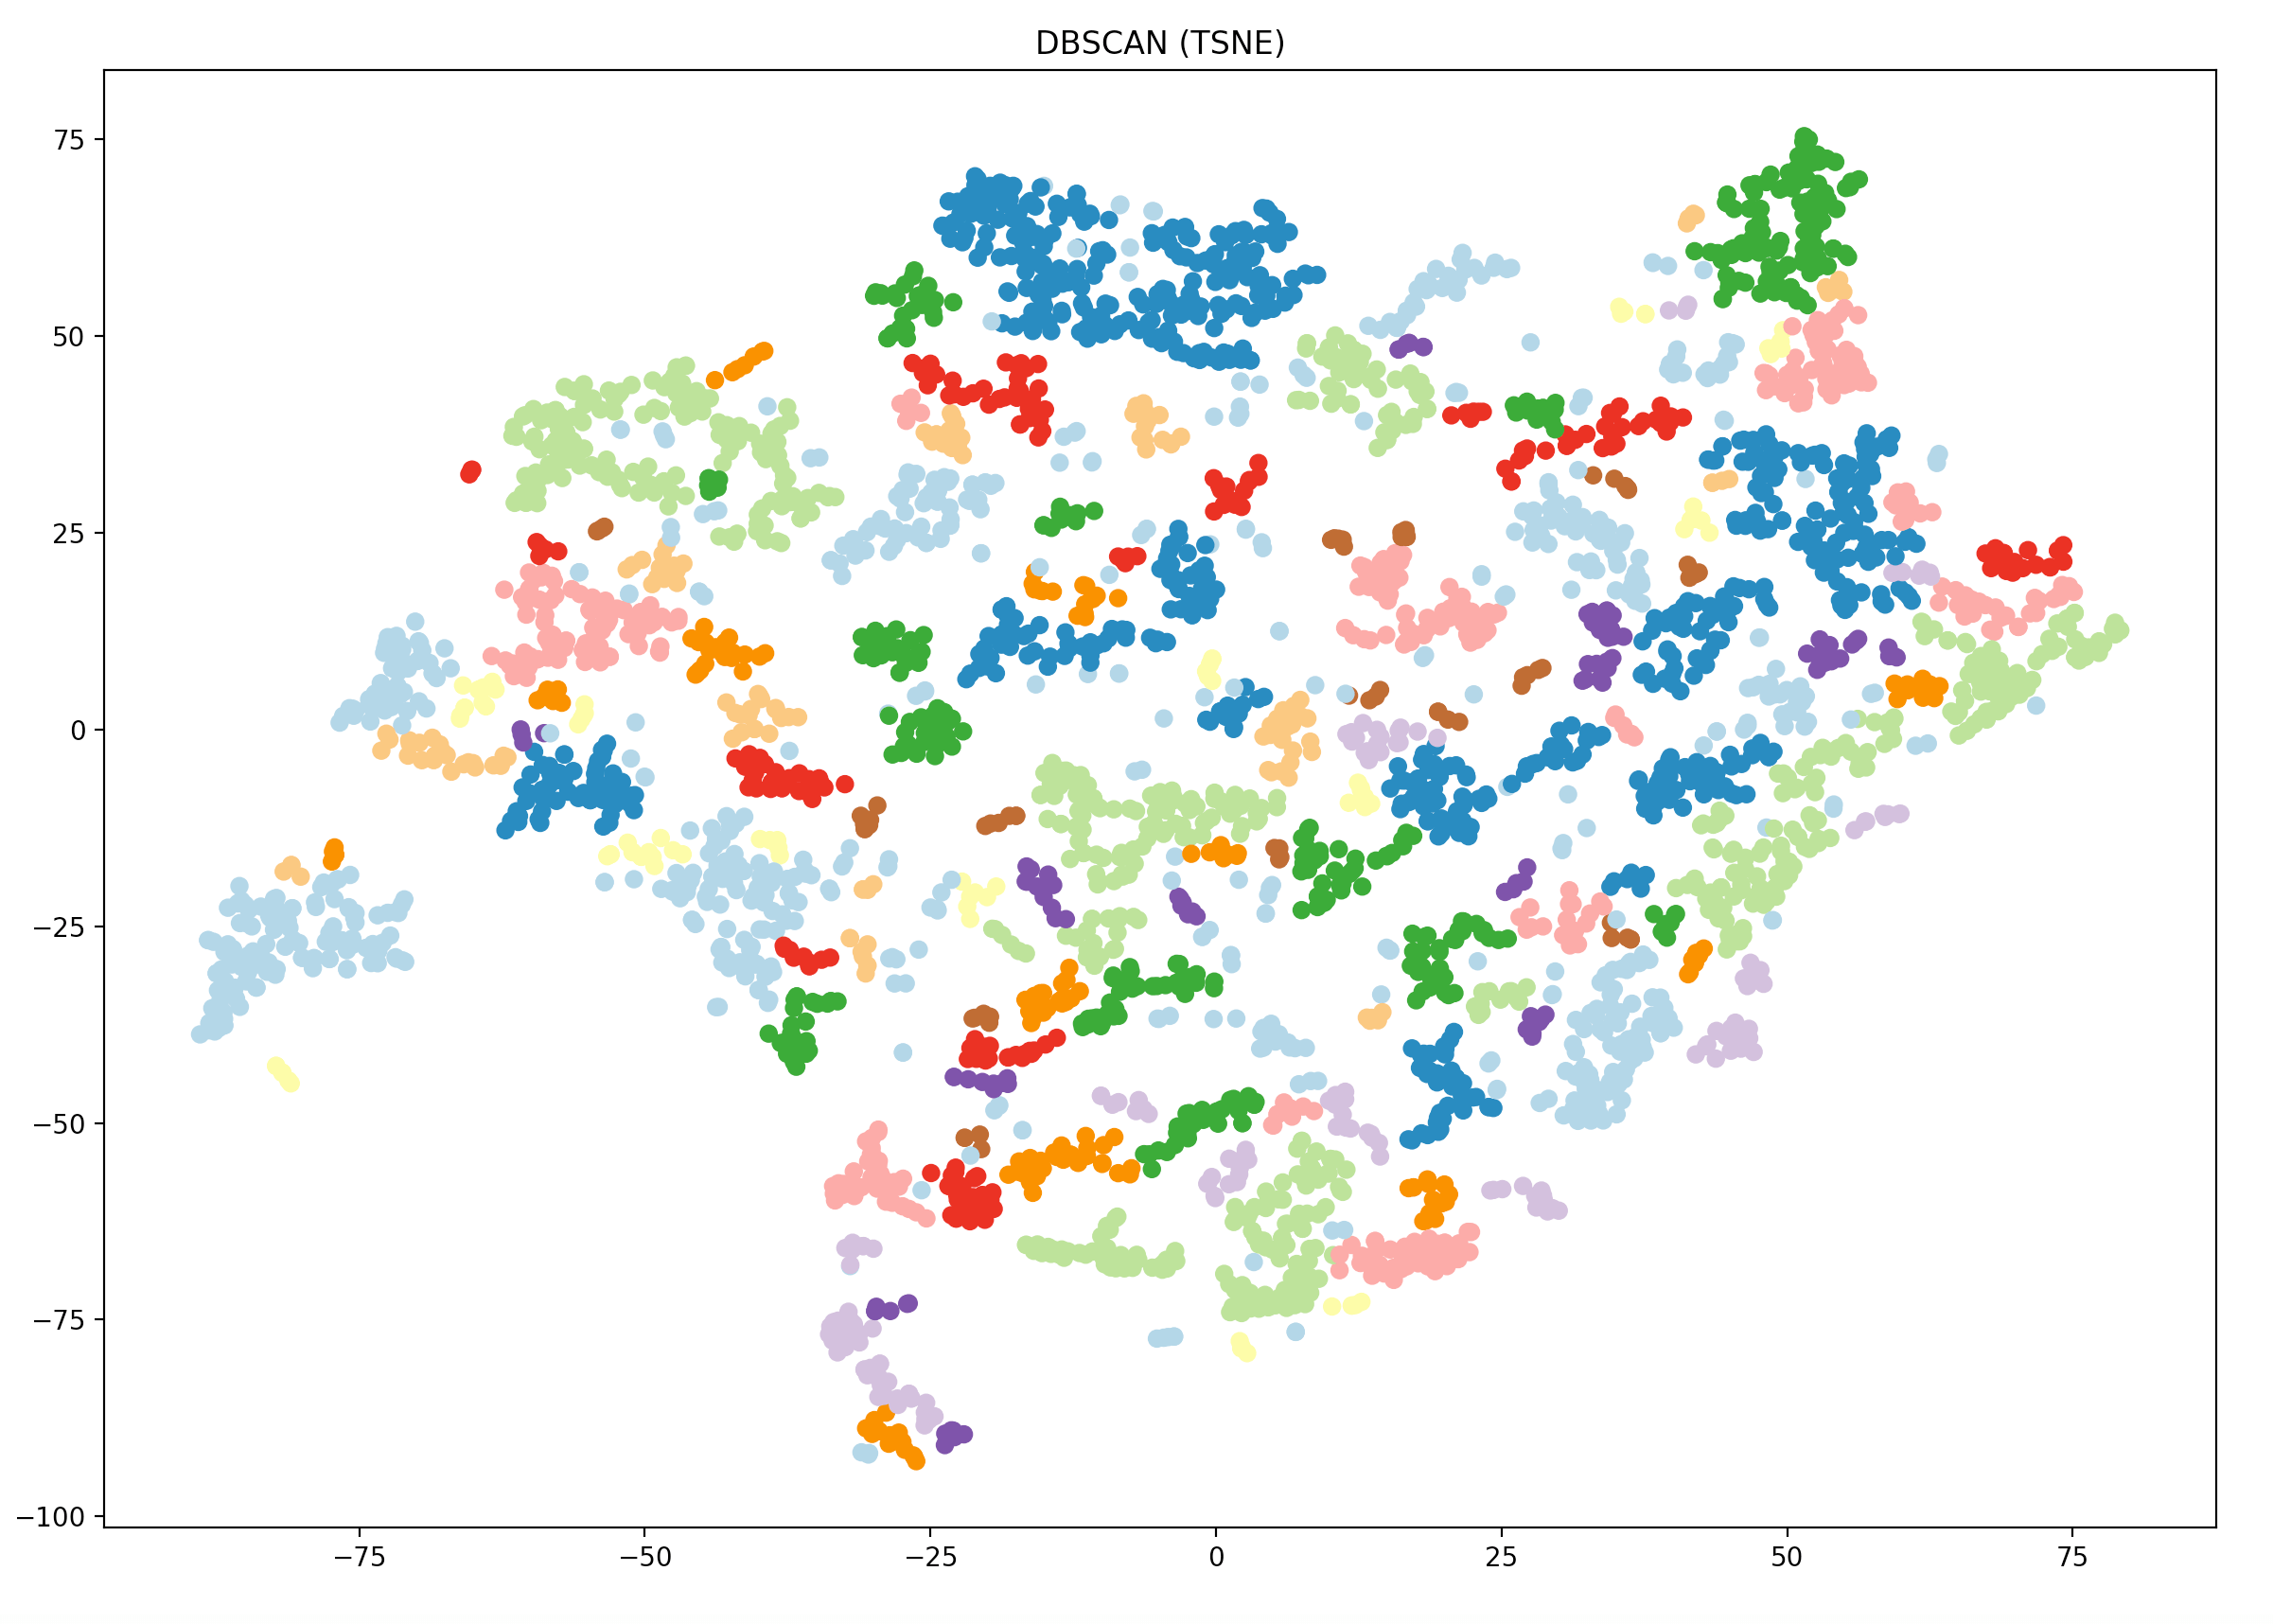
\includegraphics[width=0.9\textwidth]{./images/tsneParametersTest/perplexity/perp30-3hDBSCAN.png}
    % \caption{}
    % \label{figure:}
	\end{subfigure}
	\caption{\textbf{3h} data files, t-SNE calculated with the following parameters: \textbf{perplexity=30}, n\_iter=5000, learning\_rate=50}
  \label{figure:3hperp30TSNE}
\end{figure}



%------------------ PERPLEXITY 40: ------------------
\subsubsection{Perplexity = 40}
% -- 1h, perp 40 --
\begin{figure}[H]
  \centering
  \begin{subfigure}{.5\textwidth}
    \centering
    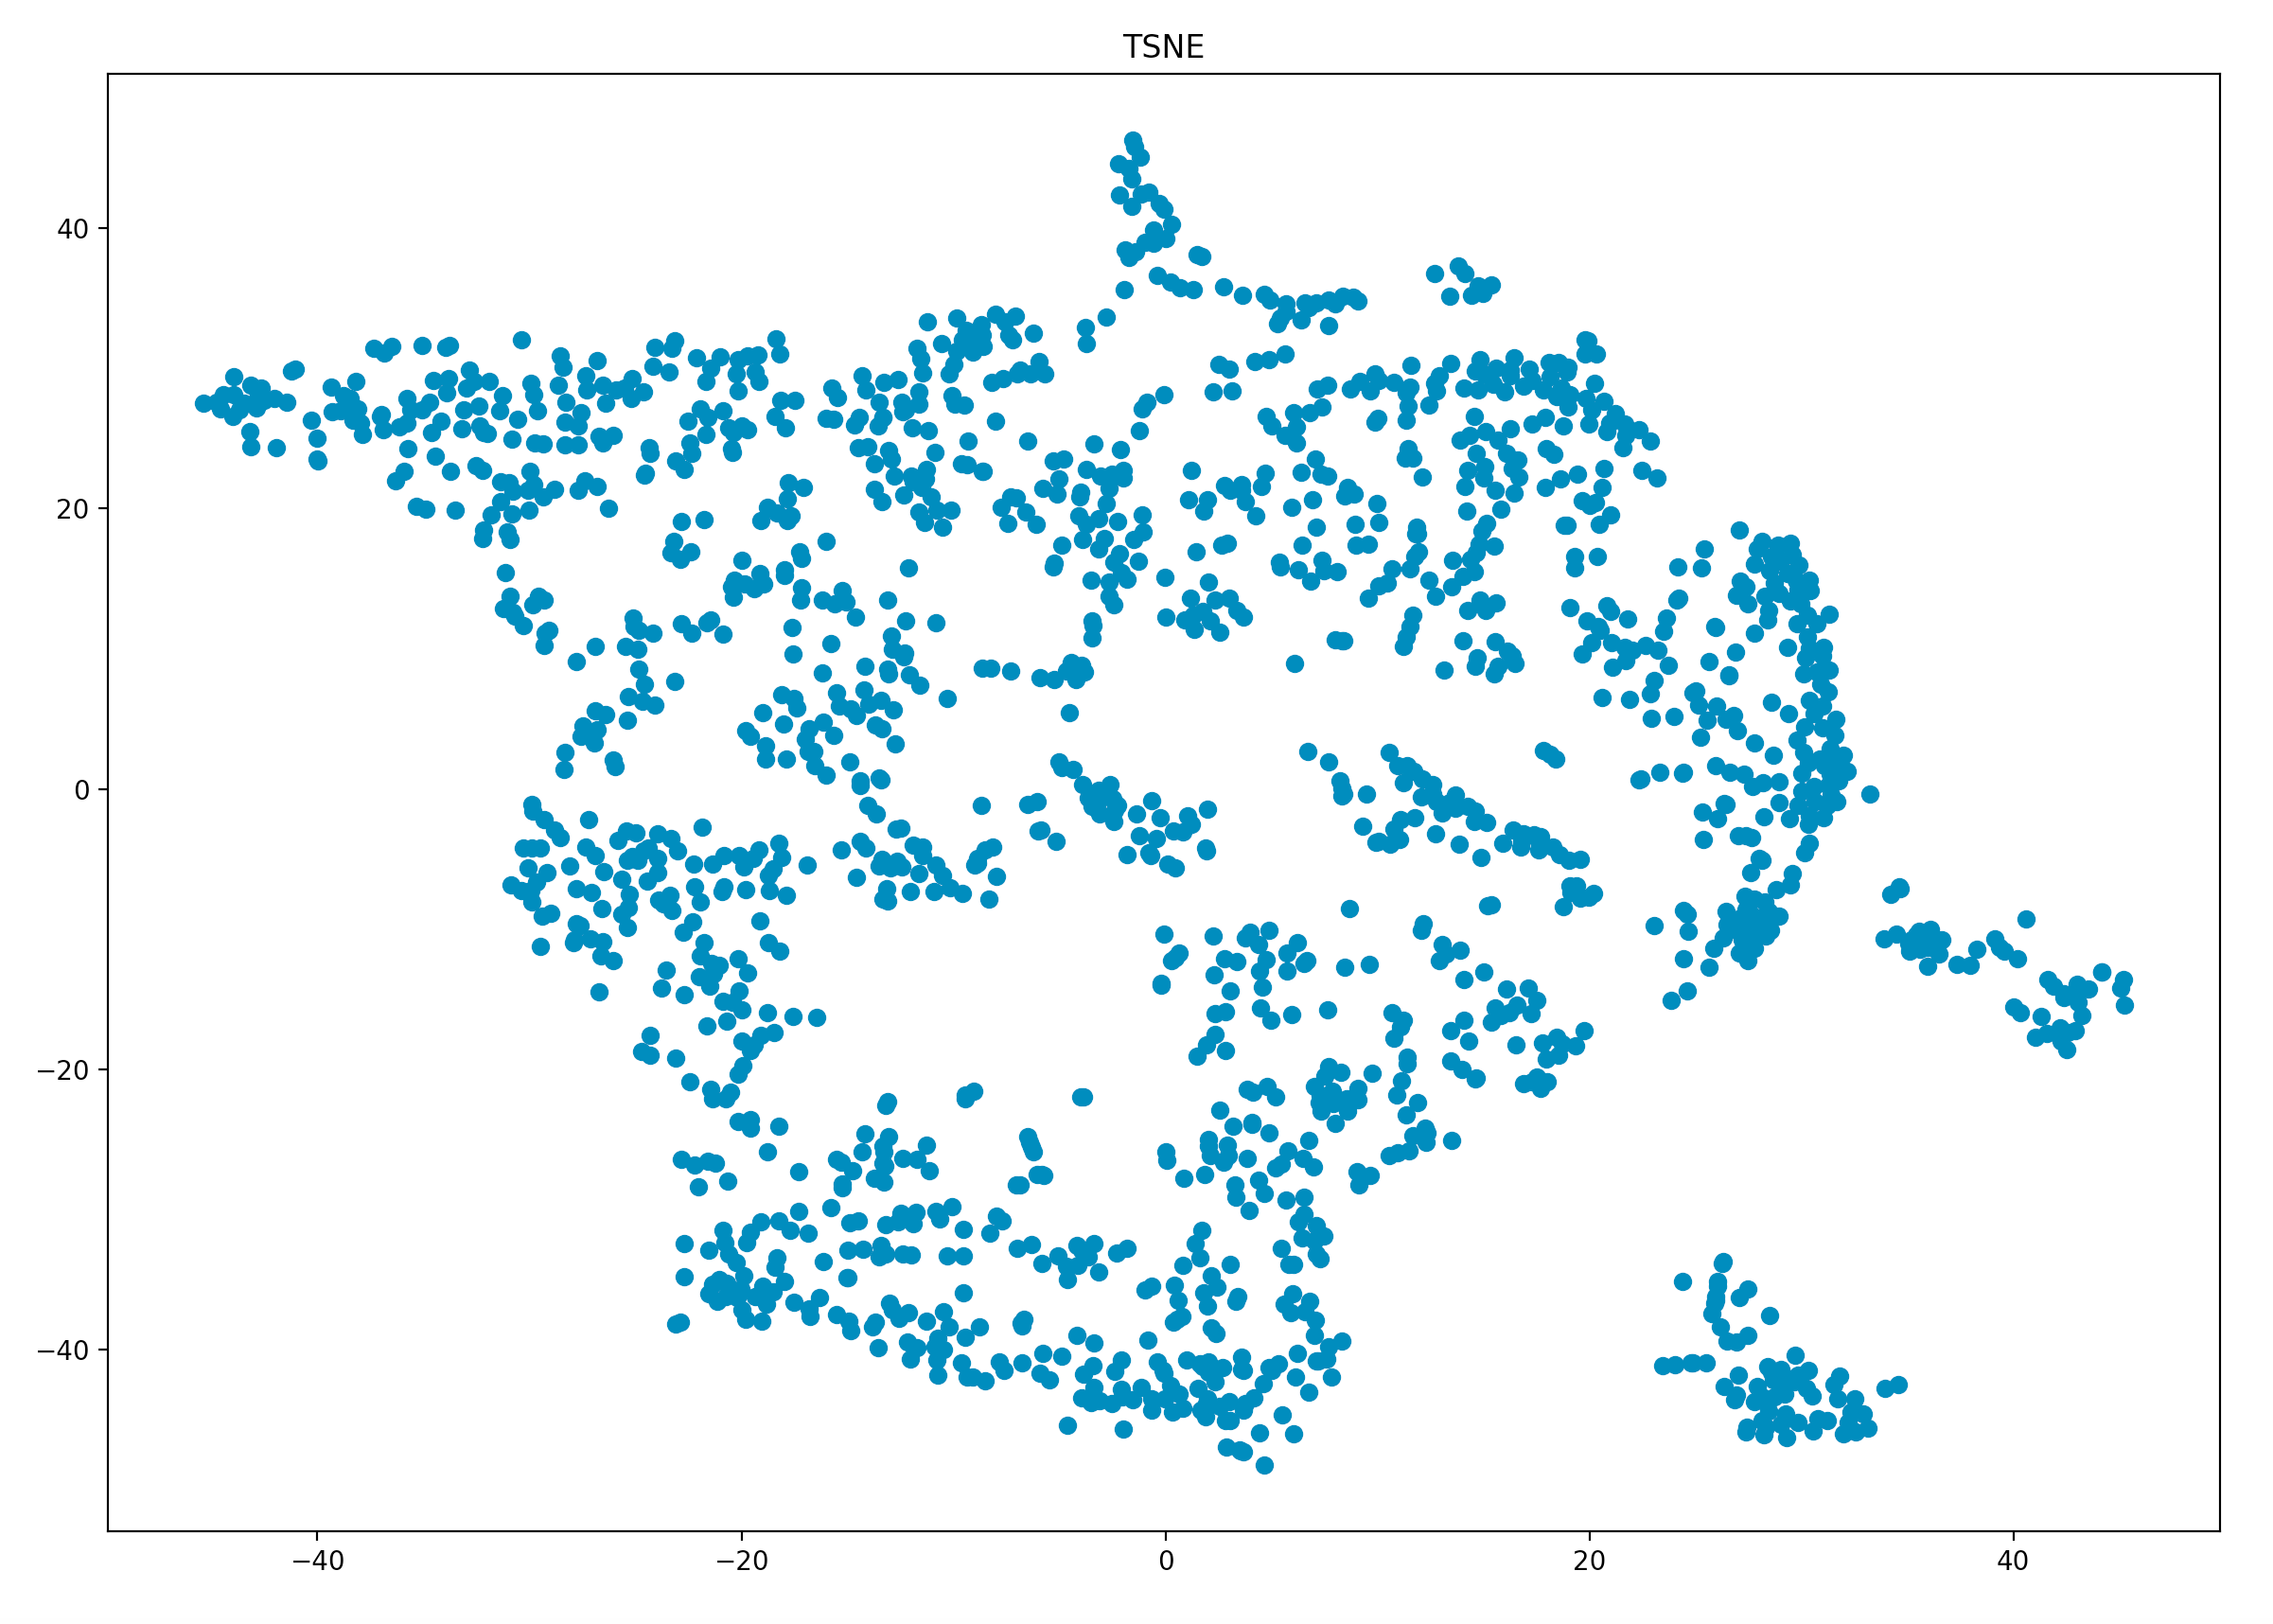
\includegraphics[width=0.9\textwidth]{./images/tsneParametersTest/perplexity/perp40-1hTSNE.png}
  % \caption{}
  % \label{figure:}
  \end{subfigure}%
  \begin{subfigure}{.5\textwidth}
    \centering
    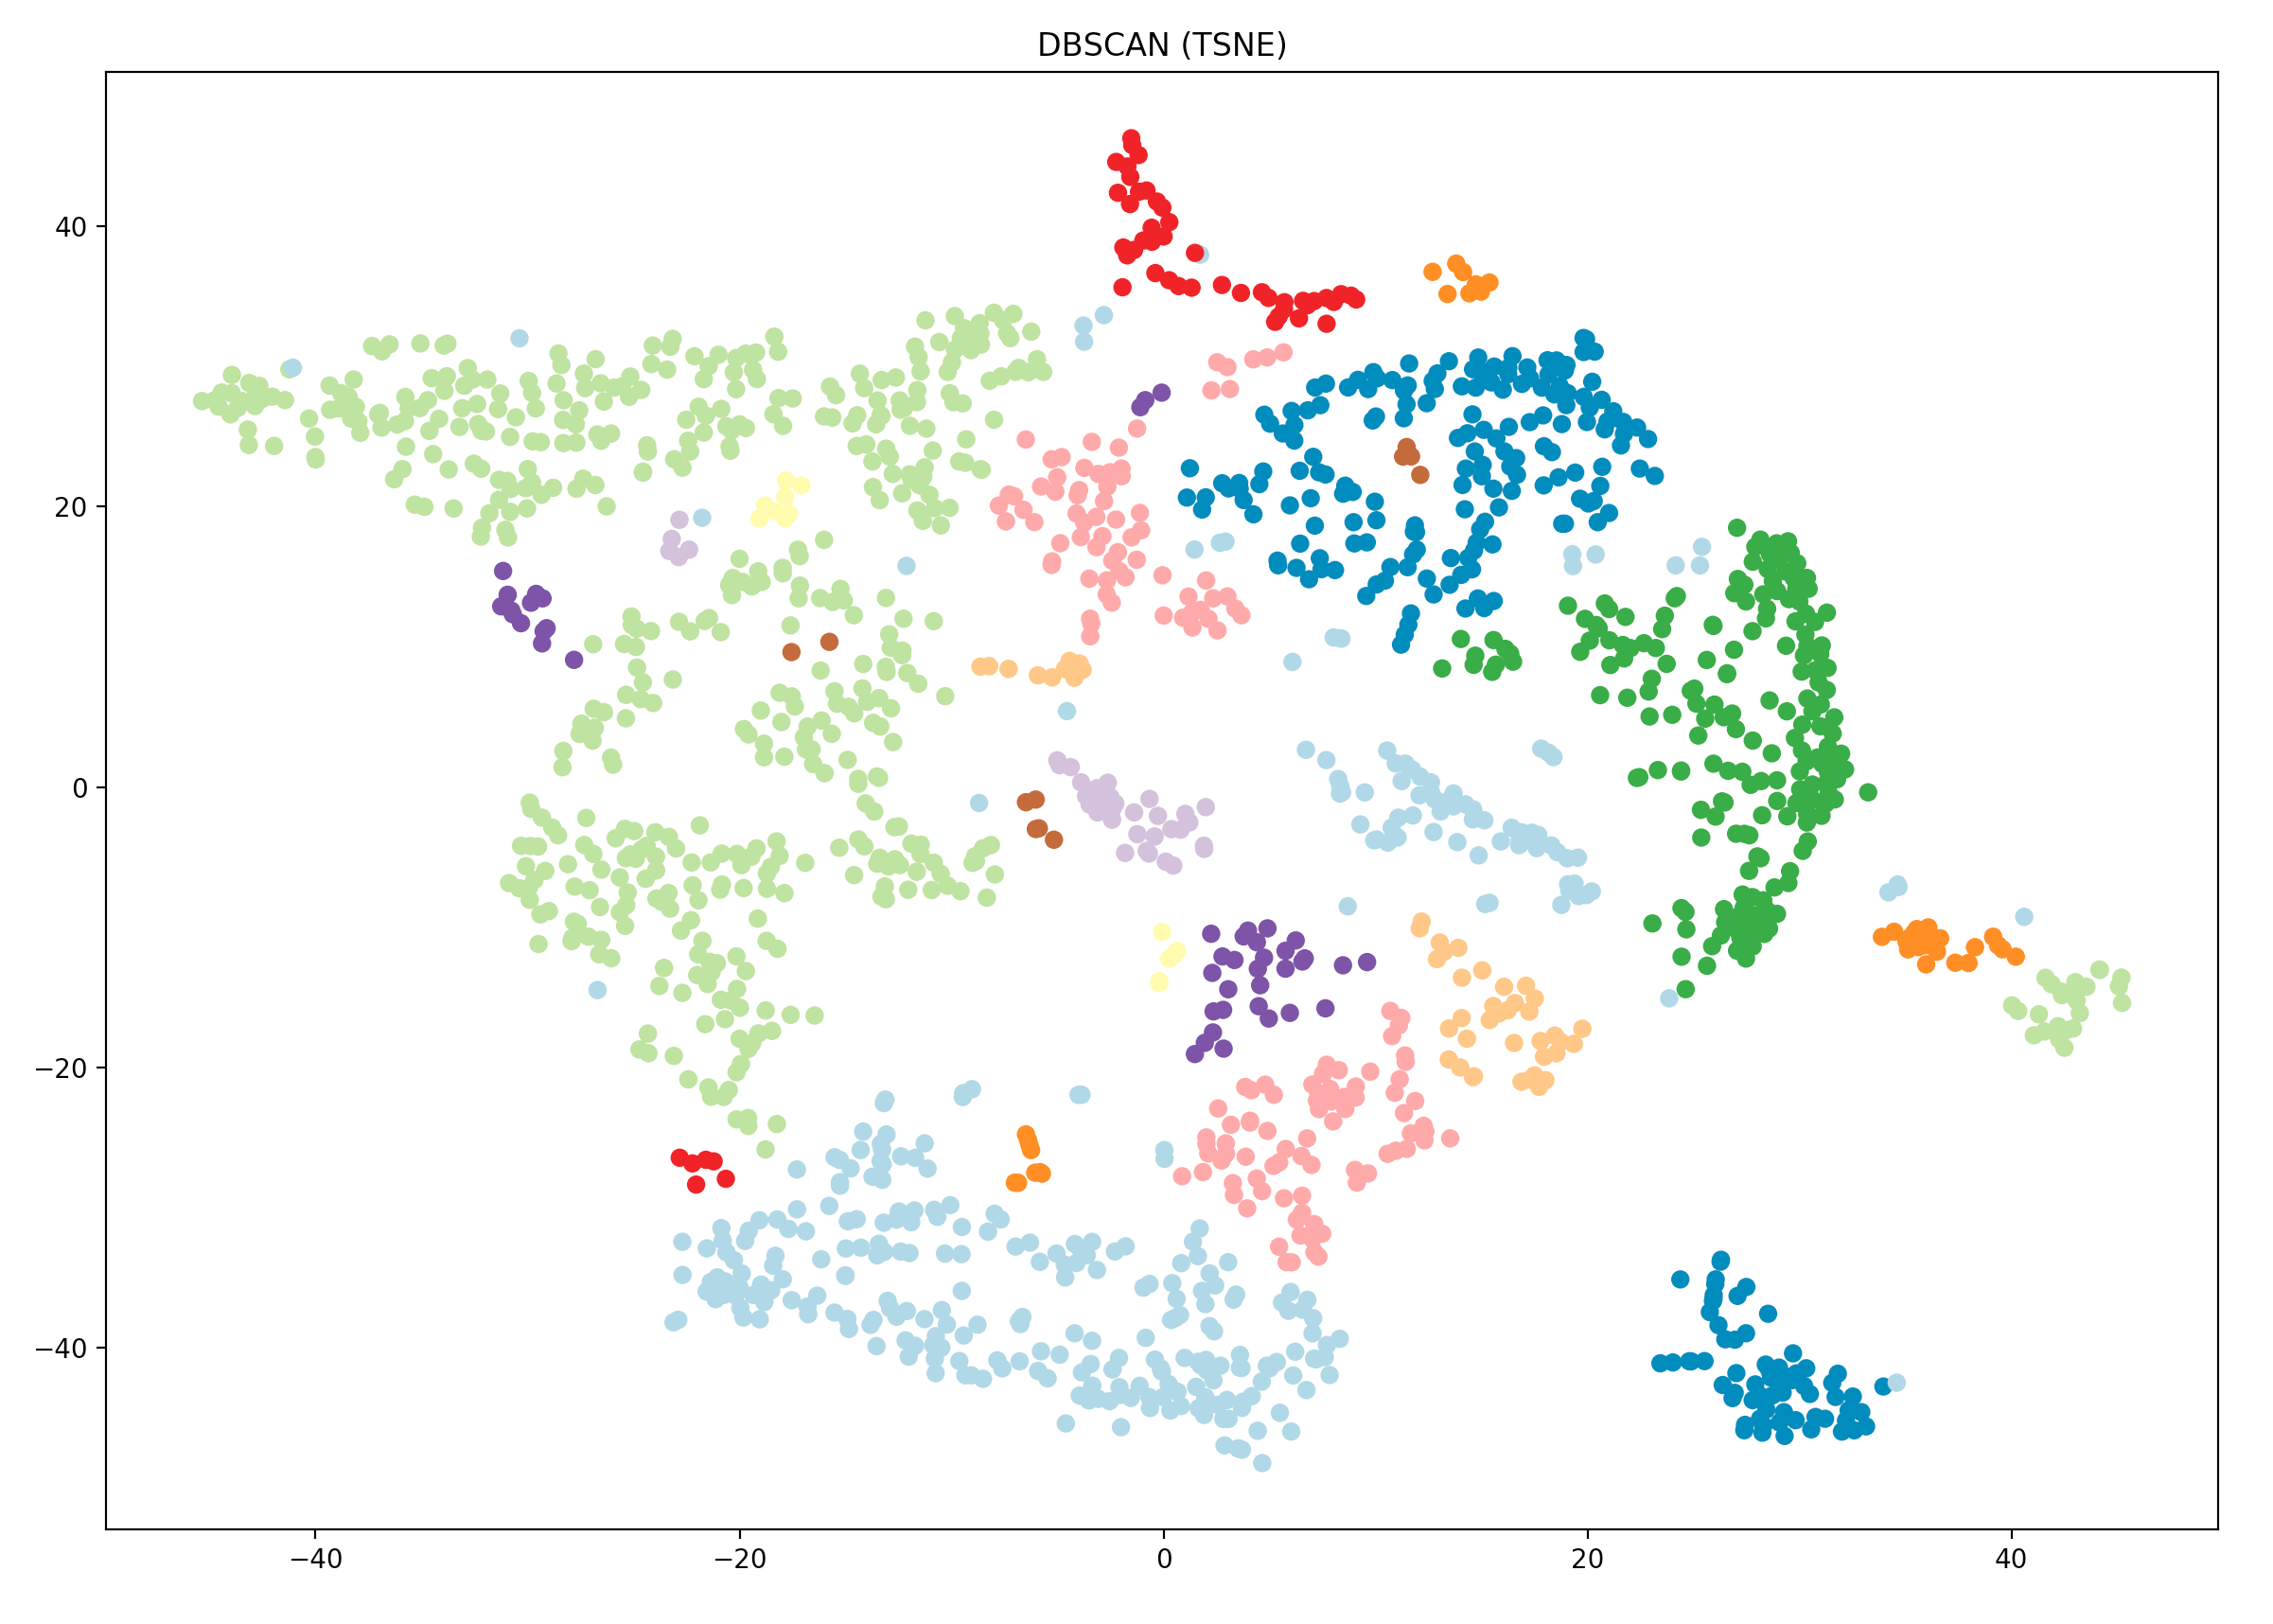
\includegraphics[width=0.9\textwidth]{./images/tsneParametersTest/perplexity/perp40-1hDBSCAN.png}
    % \caption{}
    % \label{figure:}
  \end{subfigure}
	\caption{\textbf{1h} data files, t-SNE calculated with the following parameters: \textbf{perplexity=40}, n\_iter=5000, learning\_rate=50}
  \label{figure:1hperp40TSNE}
\end{figure}

% -- 3h, perp 40 --
\begin{figure}[H]
  \centering
	\begin{subfigure}{.5\textwidth}
    \centering
    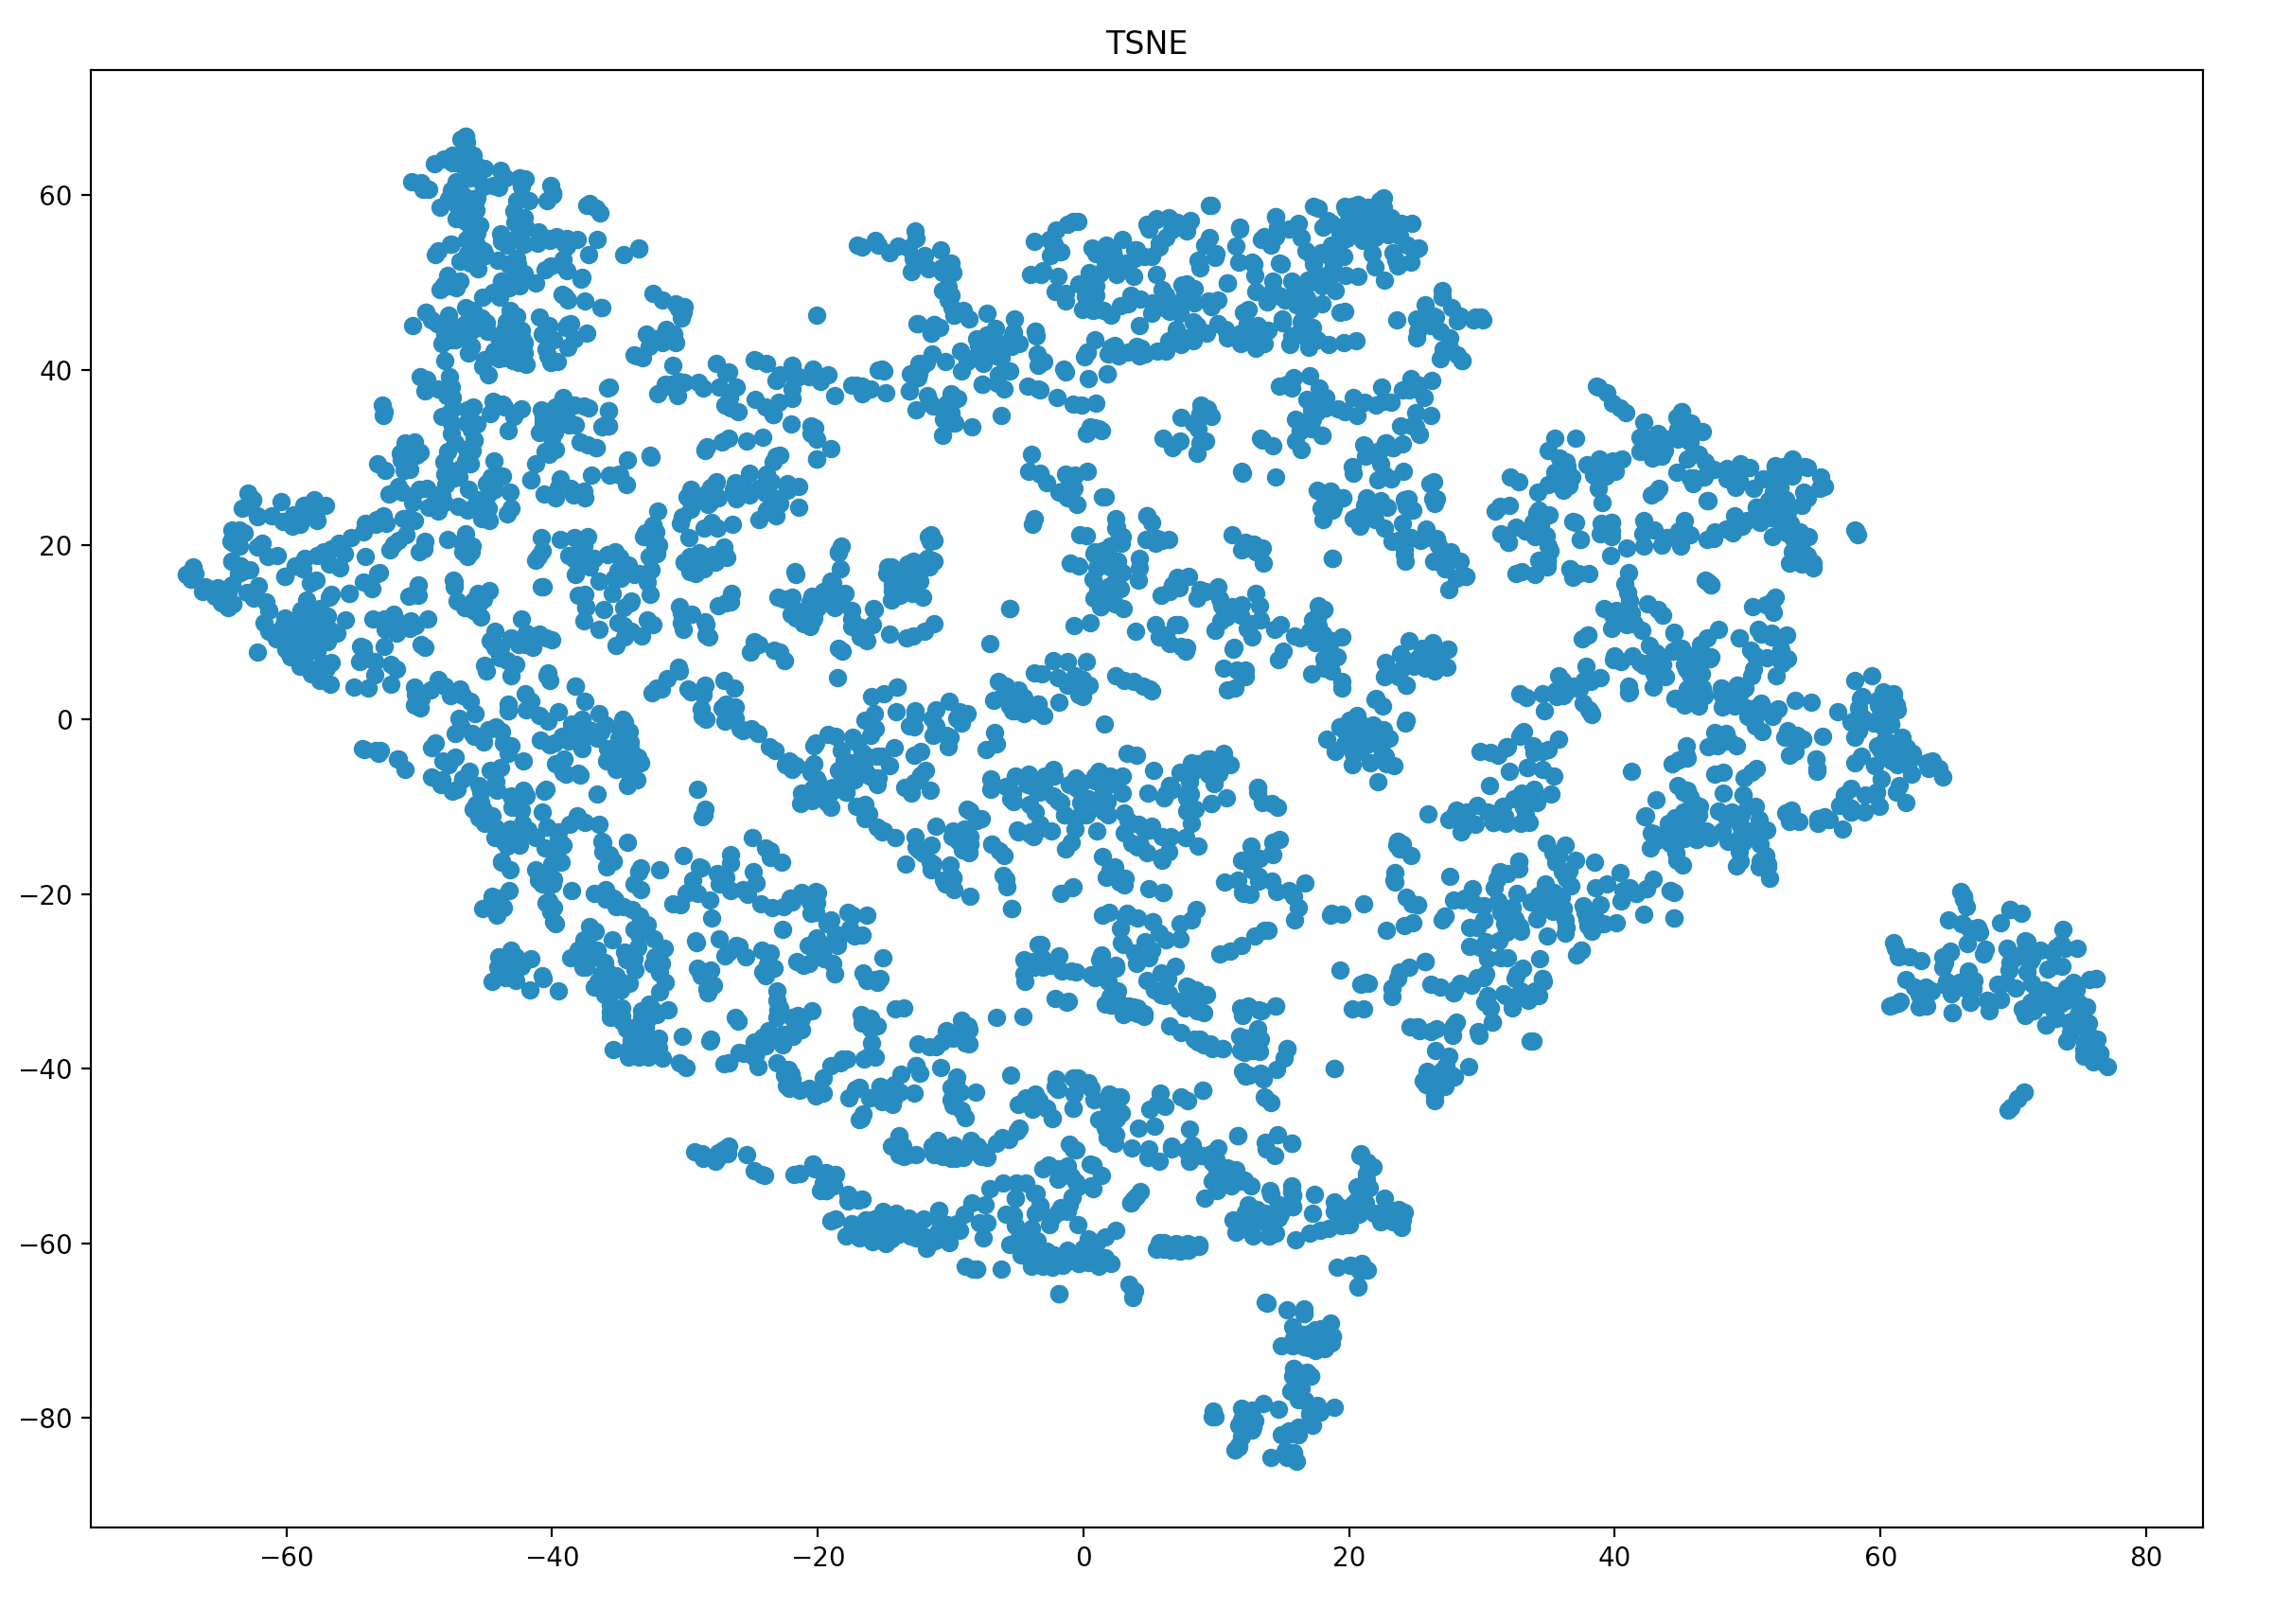
\includegraphics[width=0.9\textwidth]{./images/tsneParametersTest/perplexity/perp40-3hTSNE.png}
  % \caption{}
  % \label{figure:}
  \end{subfigure}%
  \begin{subfigure}{.5\textwidth}
    \centering
    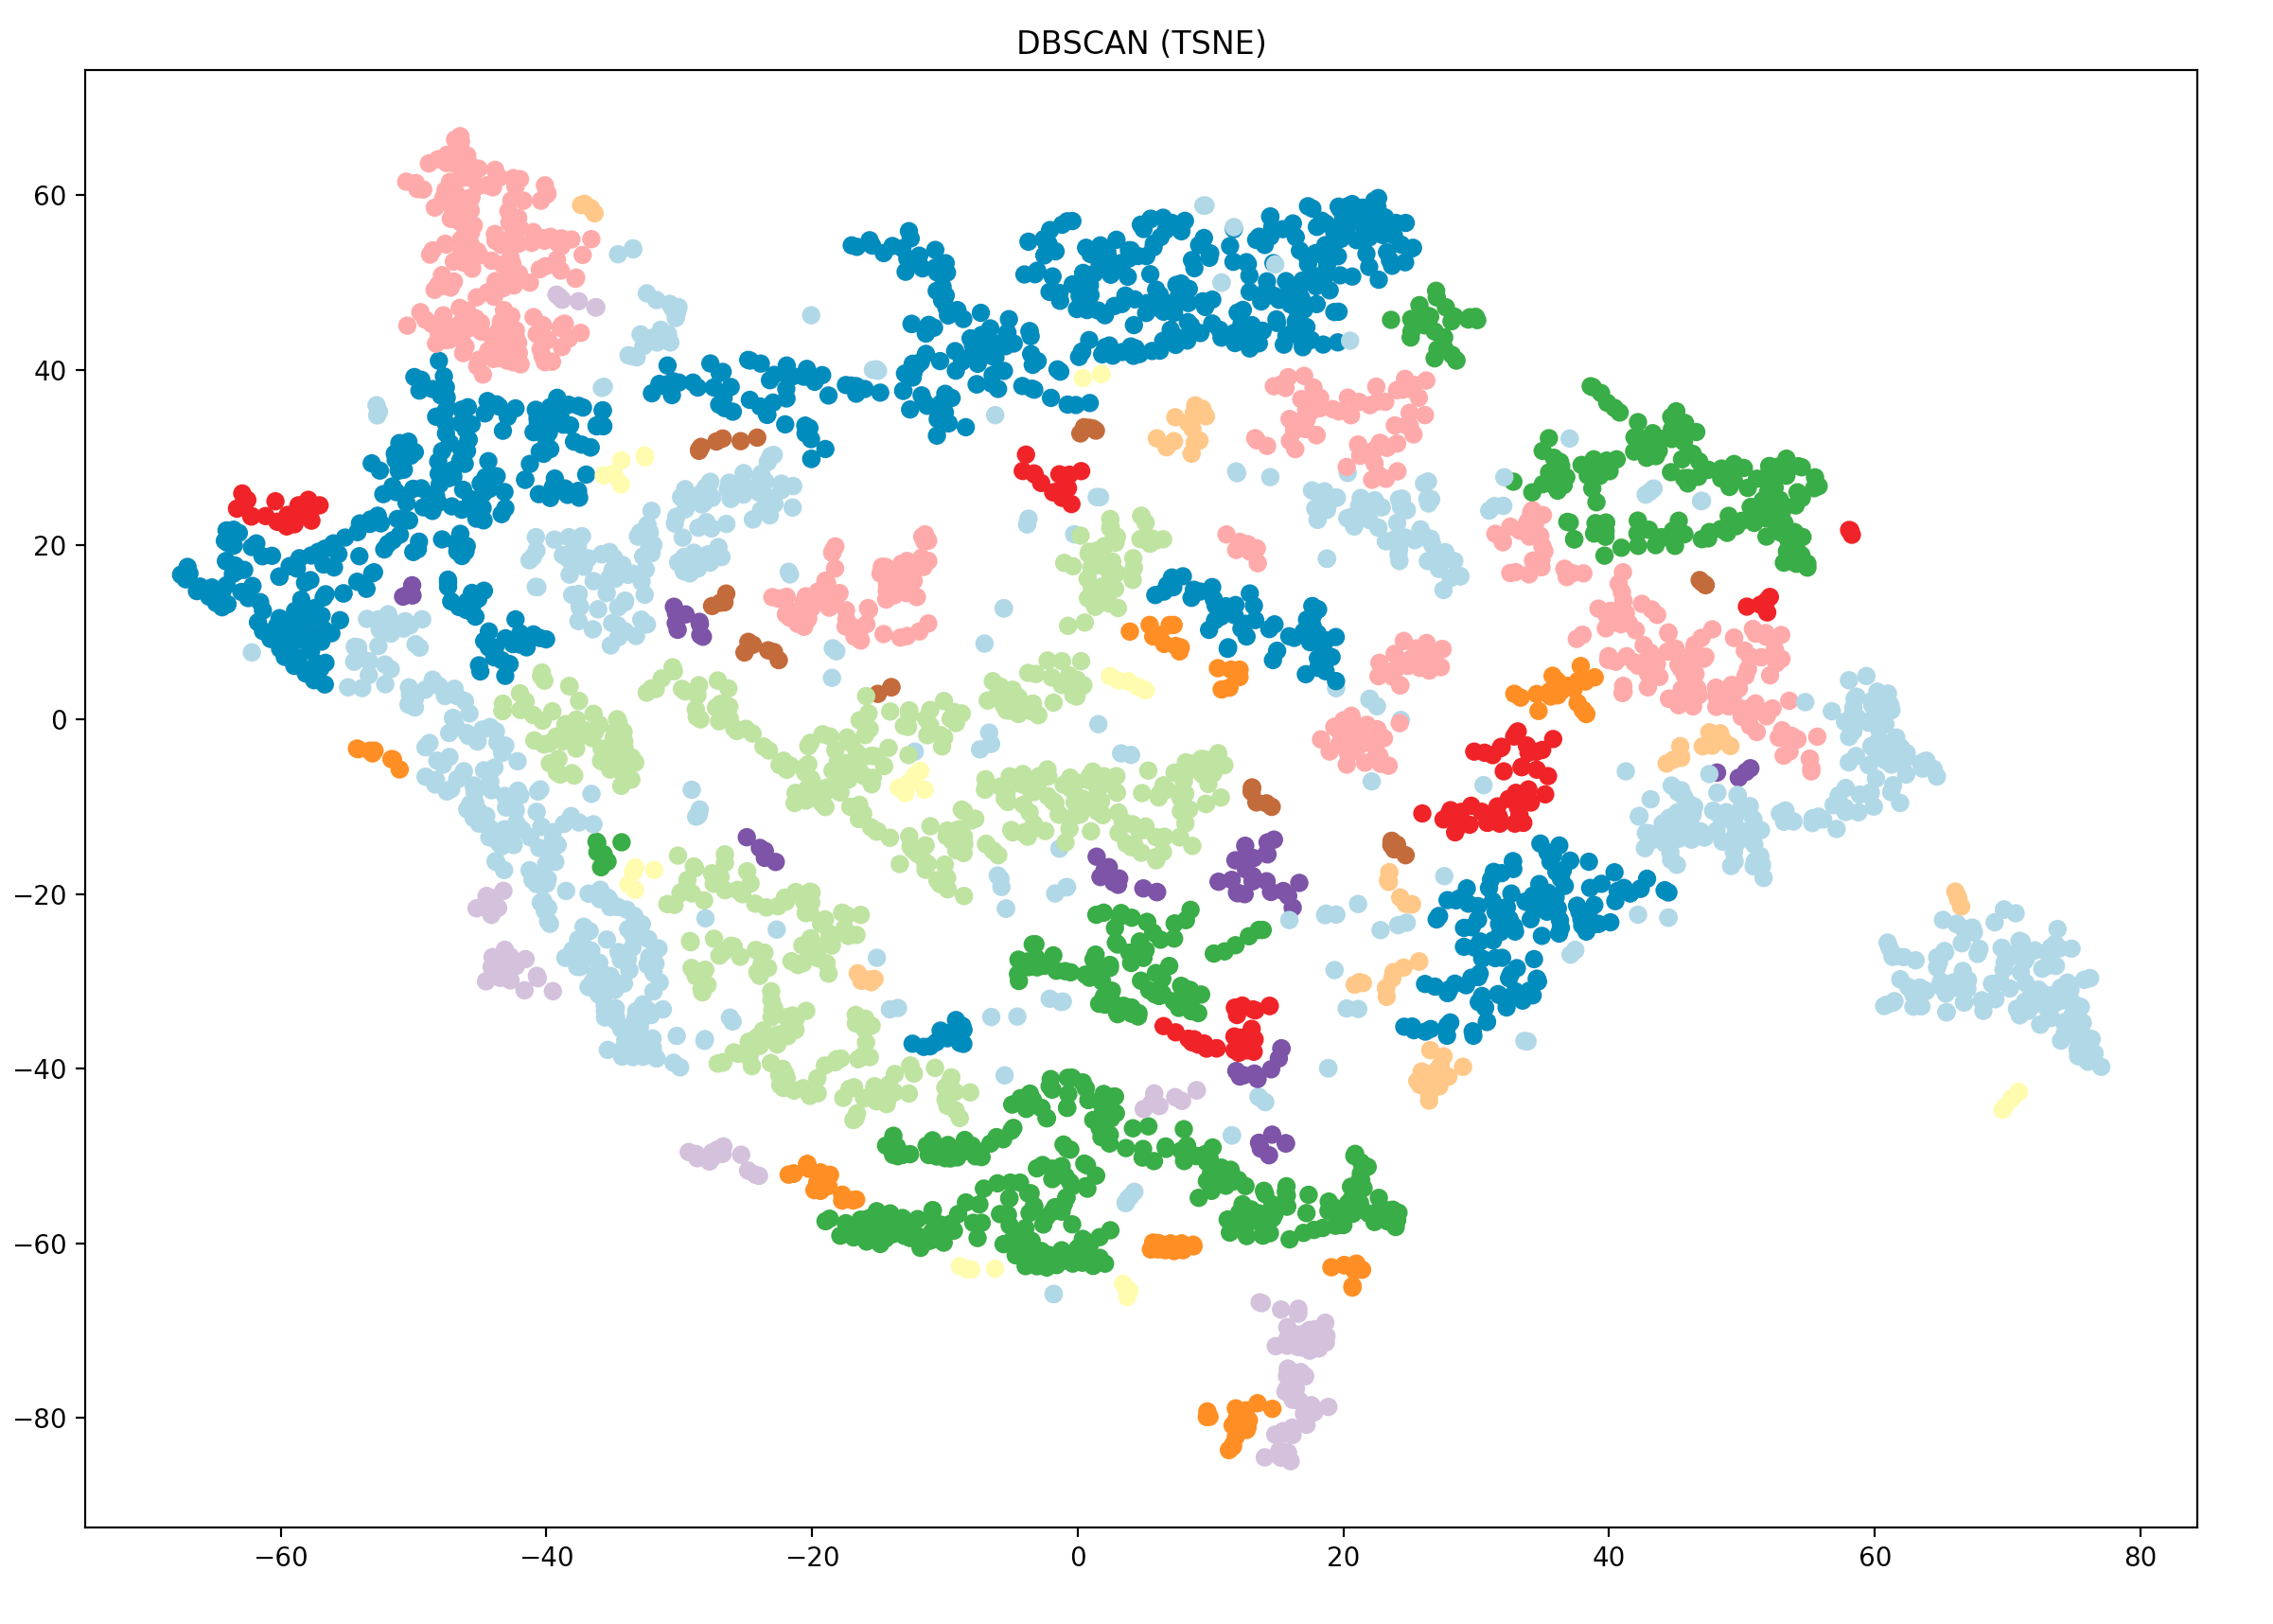
\includegraphics[width=0.9\textwidth]{./images/tsneParametersTest/perplexity/perp40-3hDBSCAN.png}
    % \caption{}
    % \label{figure:}
	\end{subfigure}
	\caption{\textbf{3h} data files, t-SNE calculated with the following parameters: \textbf{perplexity=40}, n\_iter=5000, learning\_rate=50}
  \label{figure:3hperp40TSNE}
\end{figure}



%------------------ PERPLEXITY 45: ------------------
\subsubsection{Perplexity = 45}
% -- 1h, perp 45 --
\begin{figure}[H]
  \centering
  \begin{subfigure}{.5\textwidth}
    \centering
    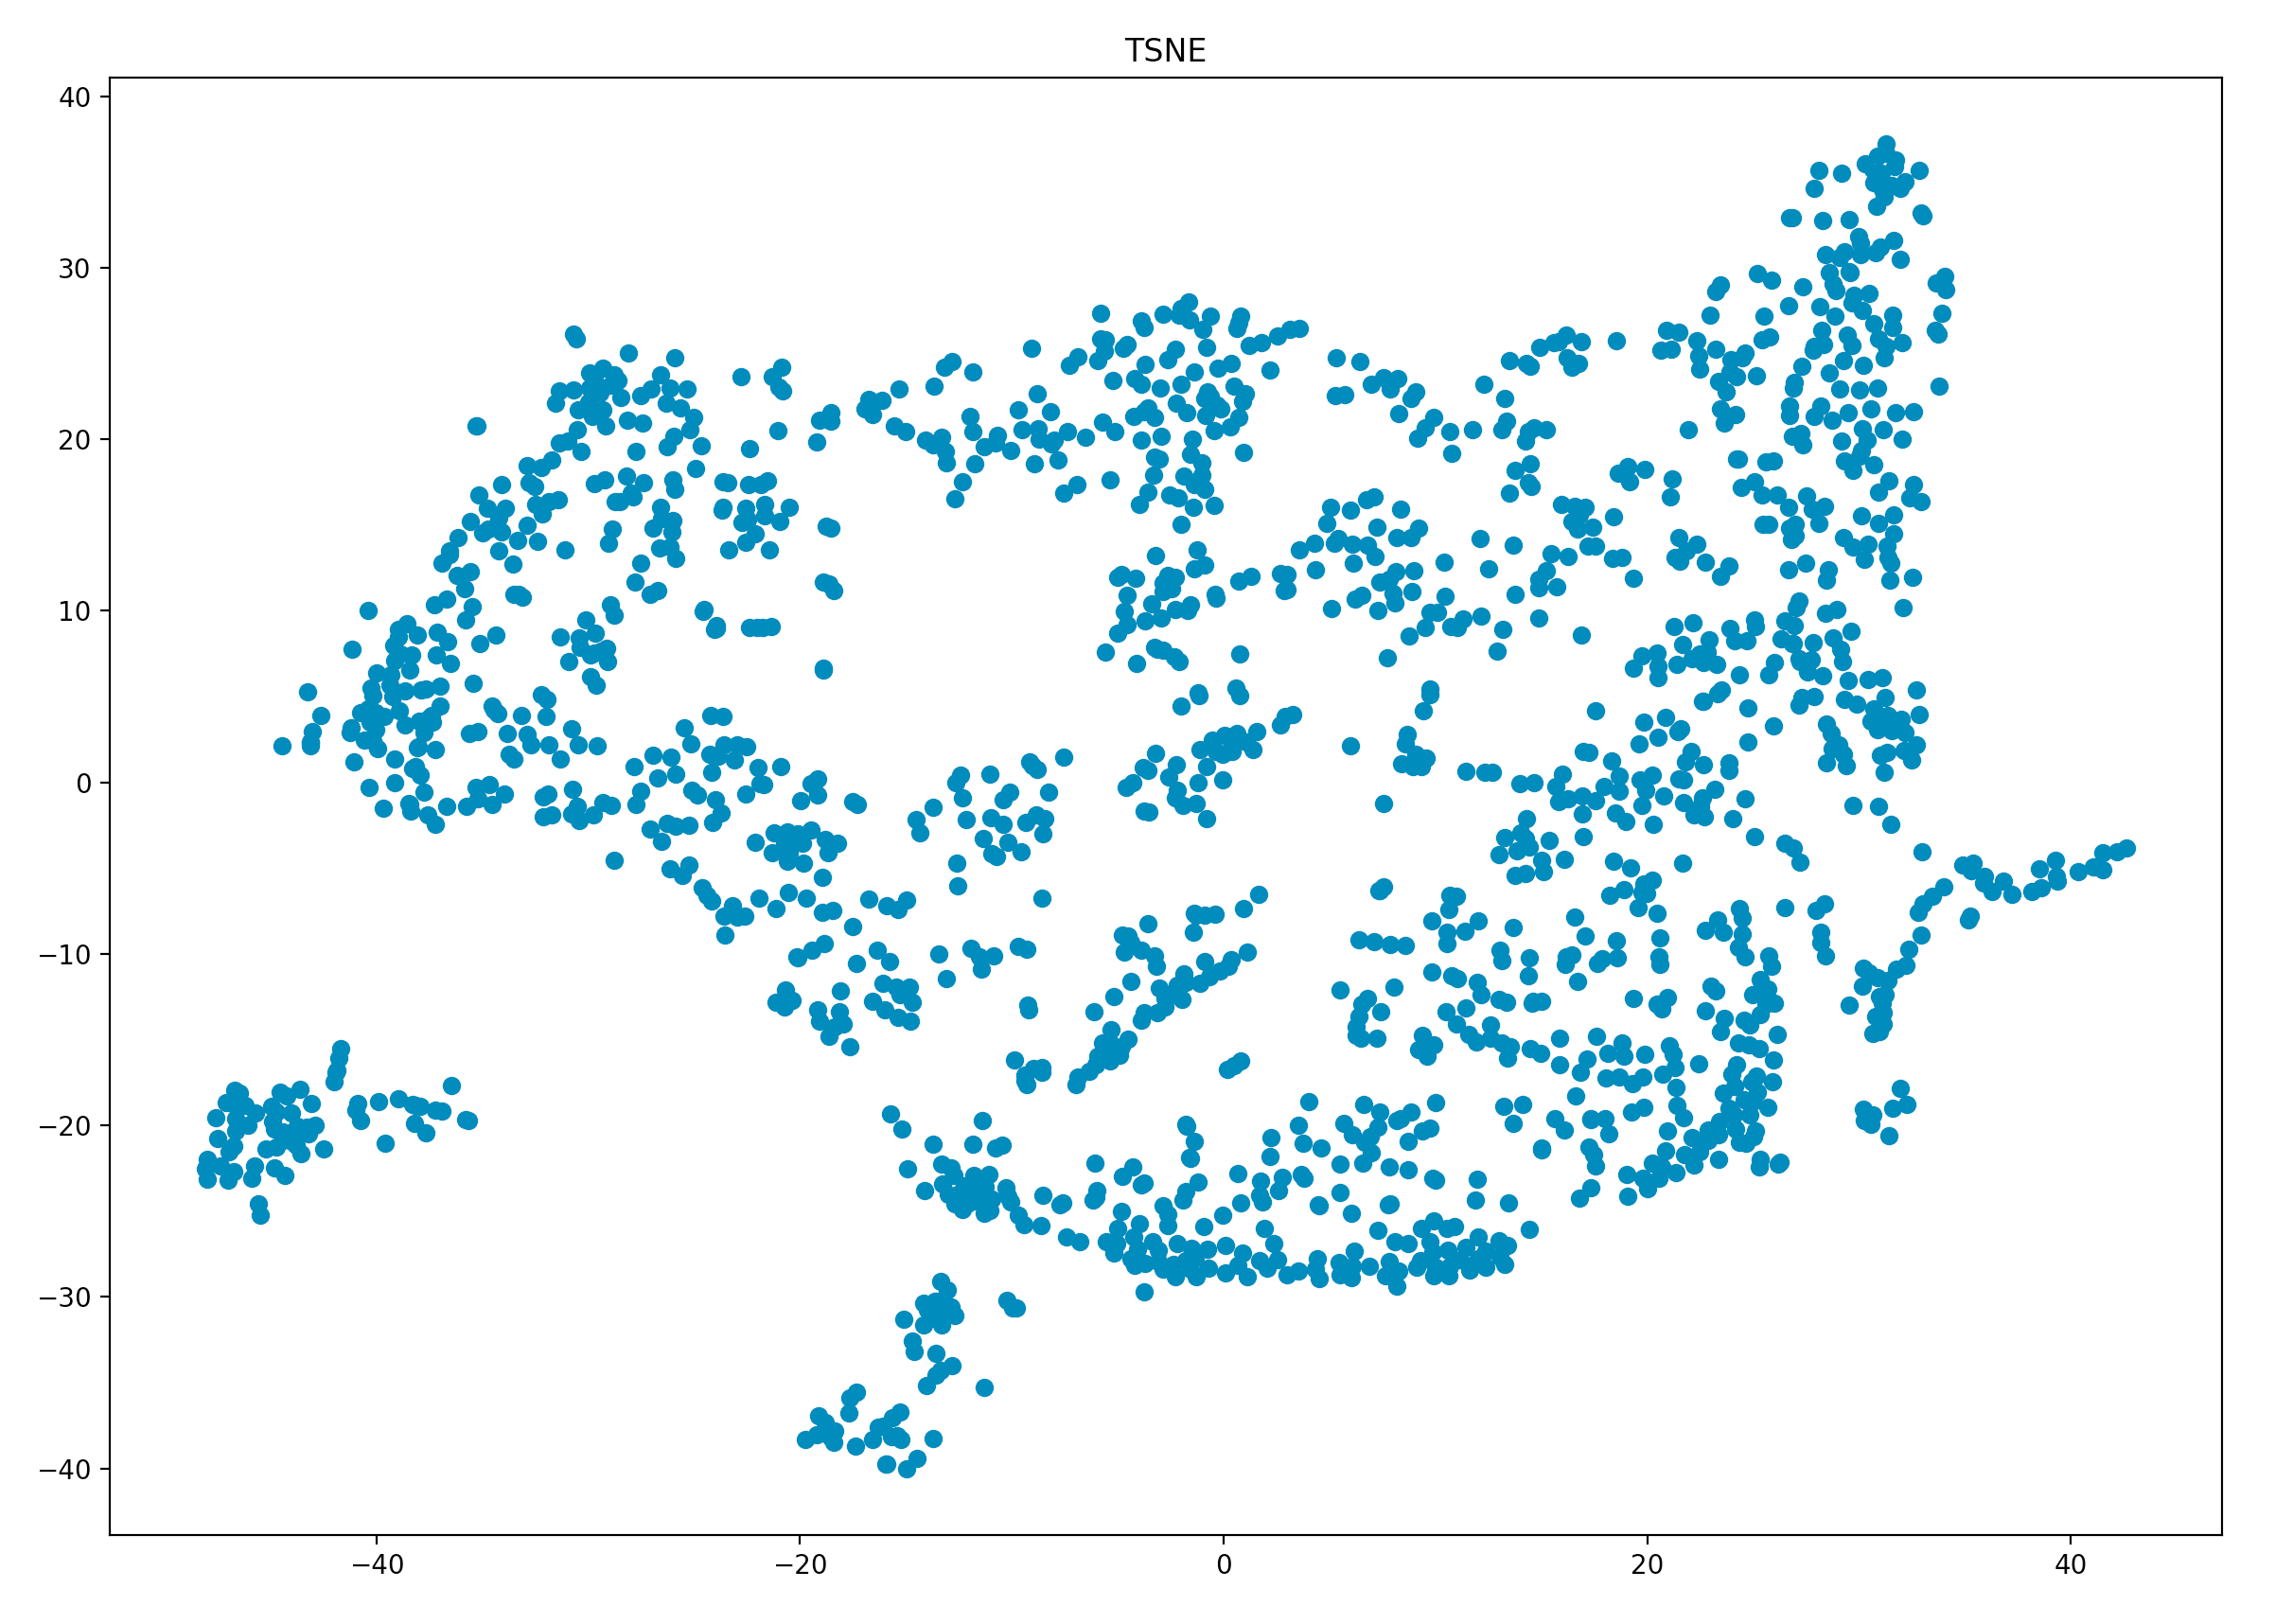
\includegraphics[width=0.9\textwidth]{./images/tsneParametersTest/perplexity/perp45-1hTSNE.png}
  % \caption{}
  % \label{figure:}
  \end{subfigure}%
  \begin{subfigure}{.5\textwidth}
    \centering
    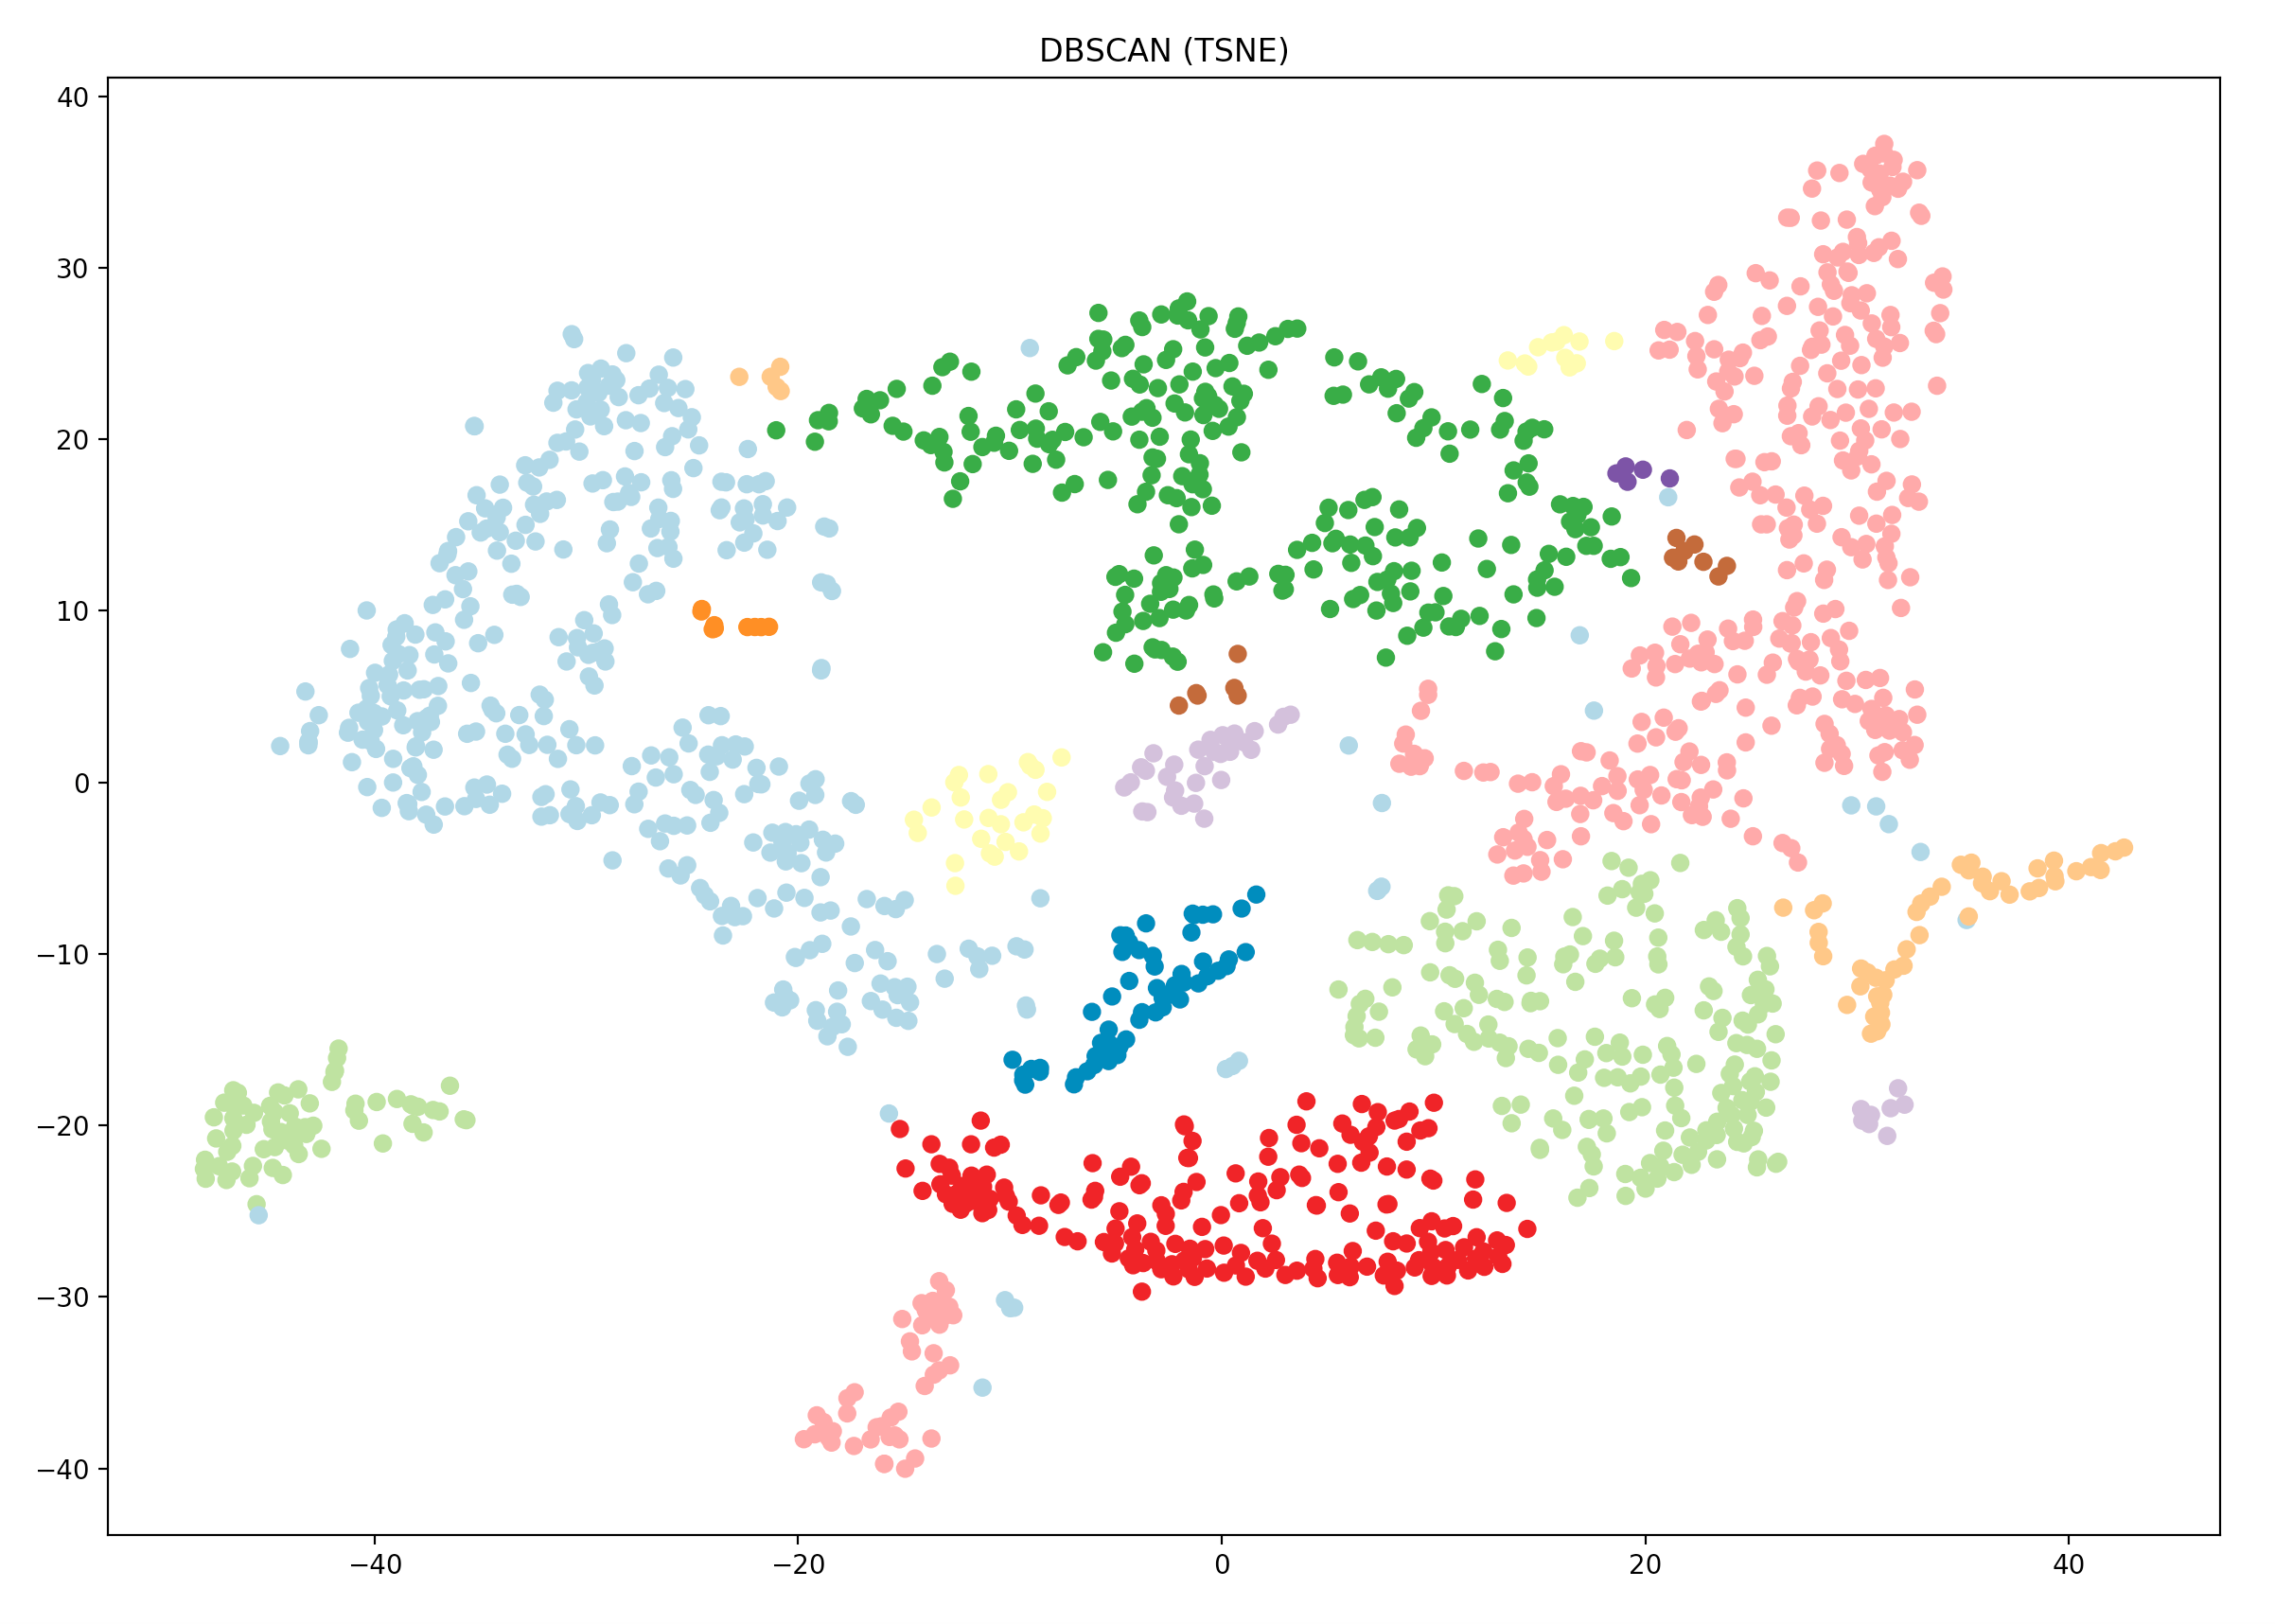
\includegraphics[width=0.9\textwidth]{./images/tsneParametersTest/perplexity/perp45-1hDBSCAN.png}
    % \caption{}
    % \label{figure:}
  \end{subfigure}
	\caption{\textbf{1h} data files, t-SNE calculated with the following parameters: \textbf{perplexity=45}, n\_iter=5000, learning\_rate=50}
  \label{figure:1hperp45TSNE}
\end{figure}

% -- 3h, perp 45 --
\begin{figure}[H]
  \centering
	\begin{subfigure}{.5\textwidth}
    \centering
    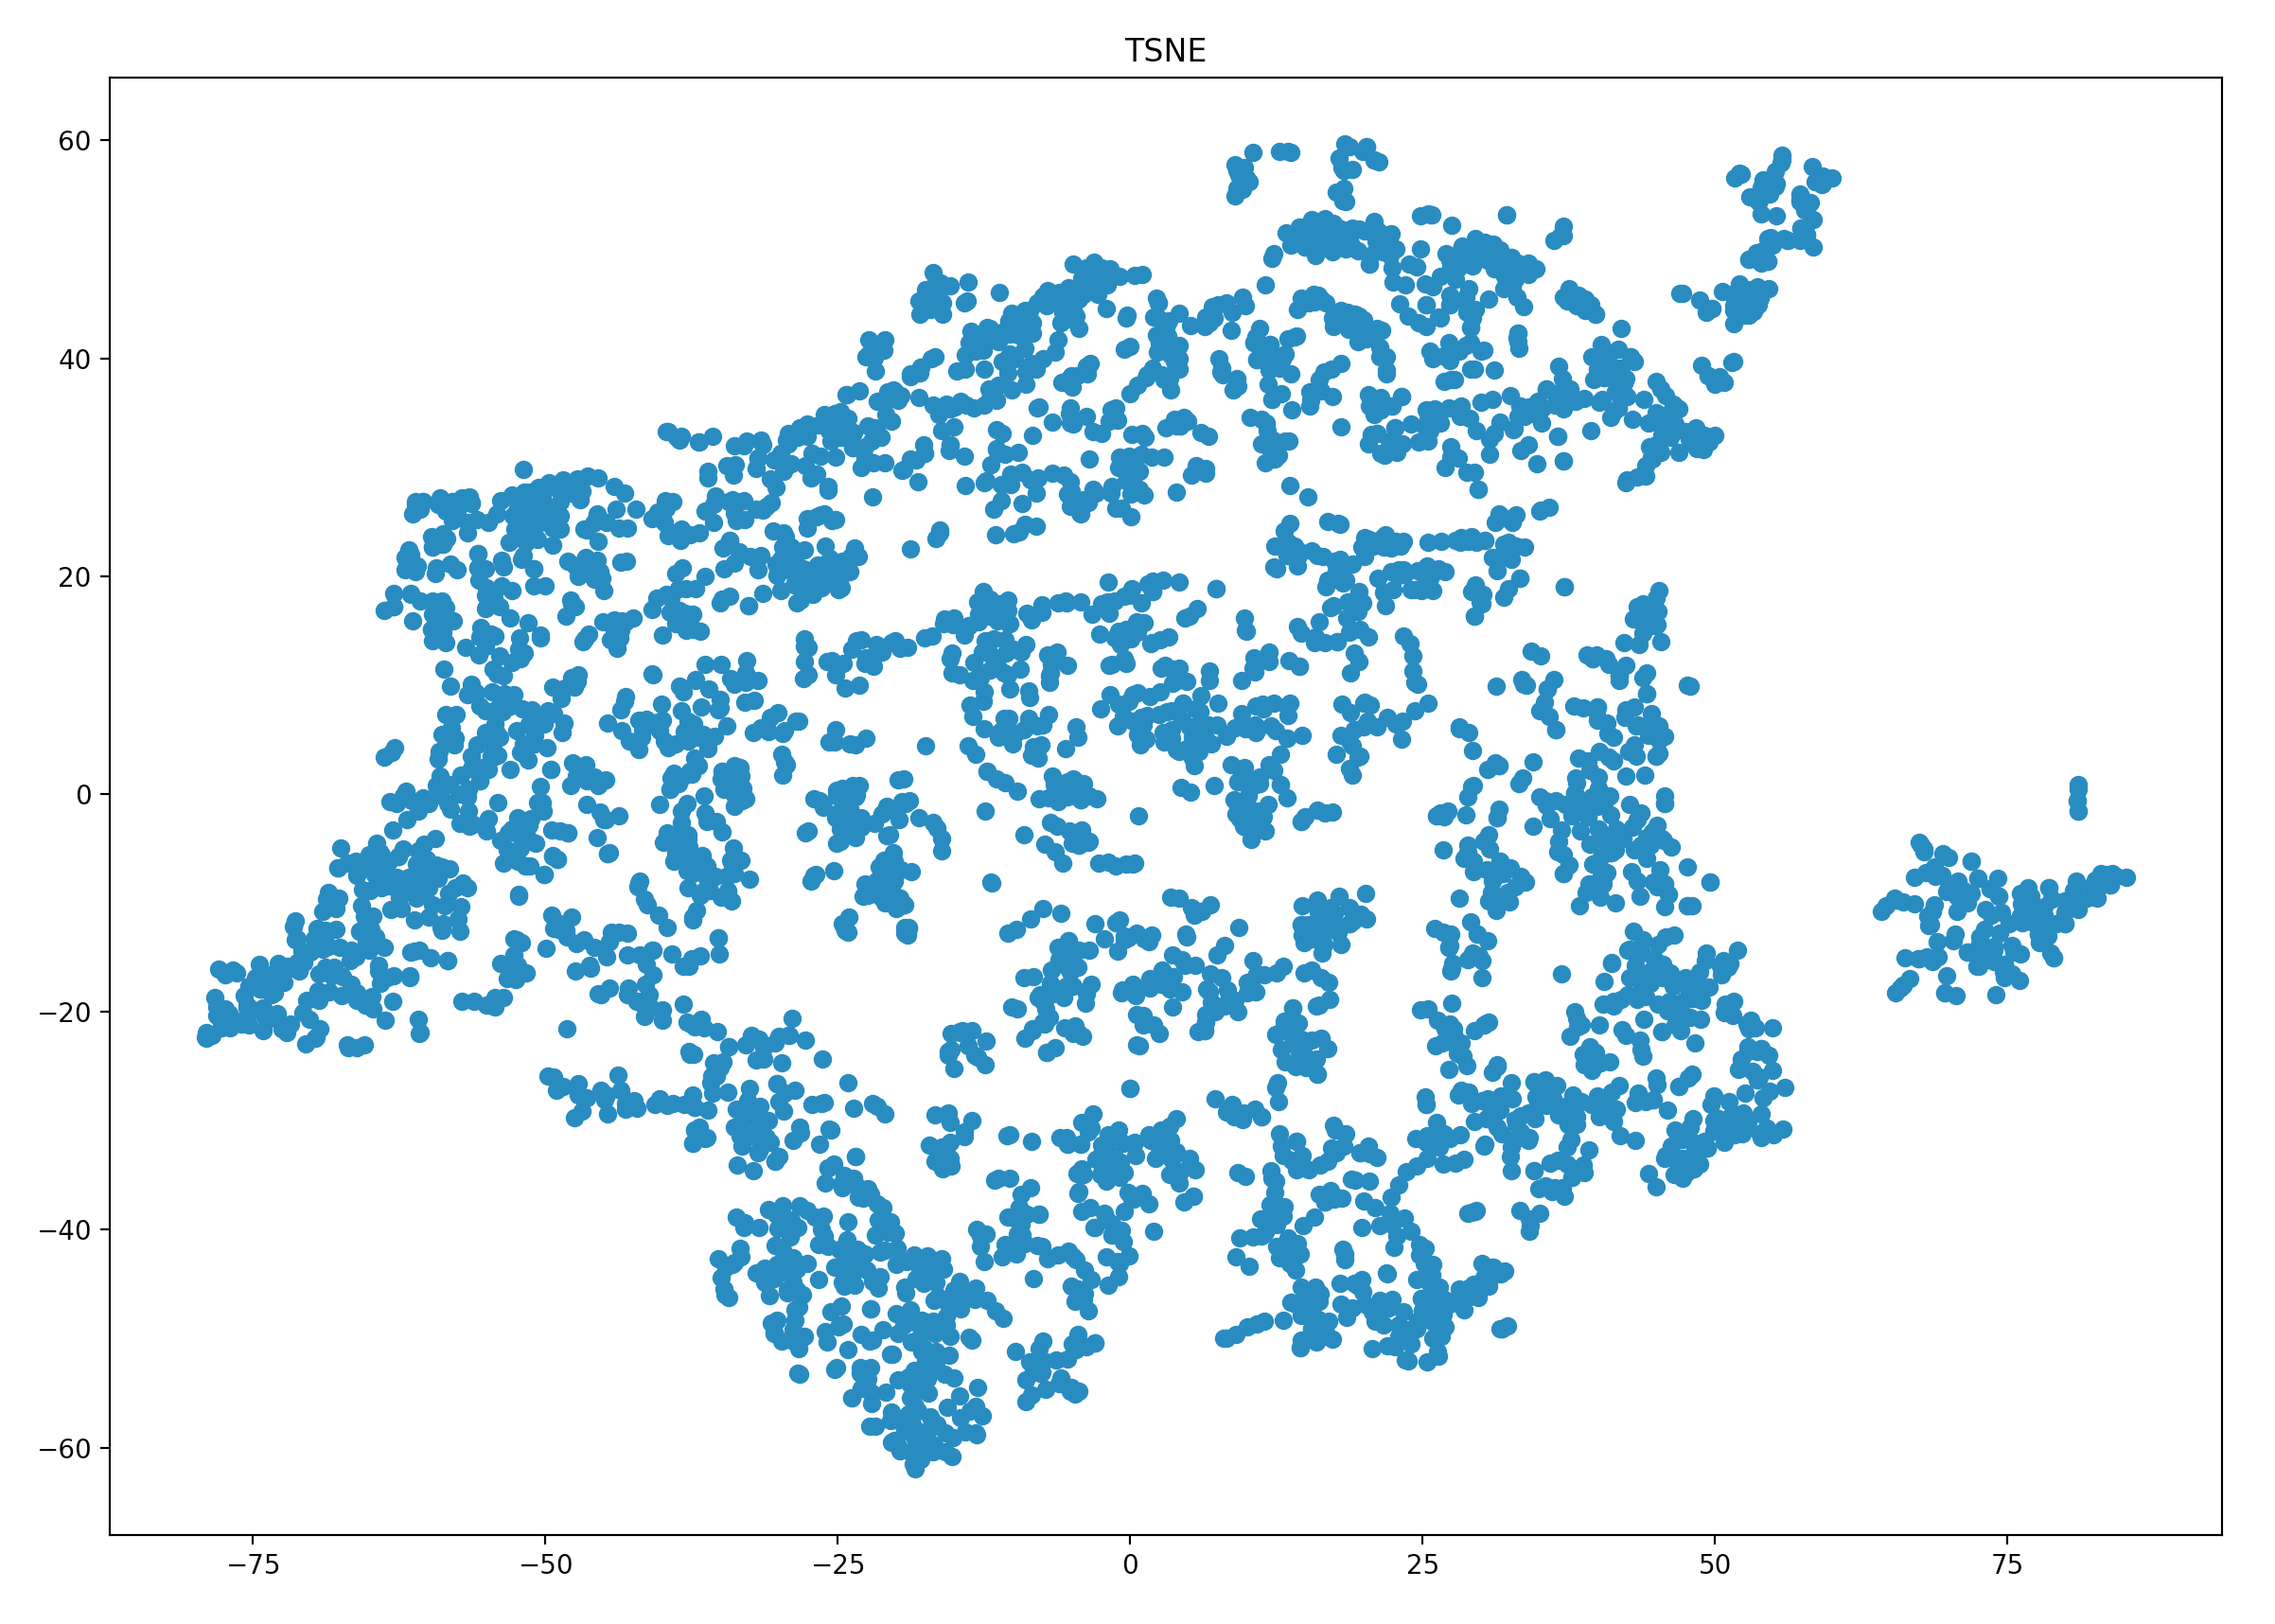
\includegraphics[width=0.9\textwidth]{./images/tsneParametersTest/perplexity/perp45-3hTSNE.png}
  % \caption{}
  % \label{figure:}
  \end{subfigure}%
  \begin{subfigure}{.5\textwidth}
    \centering
    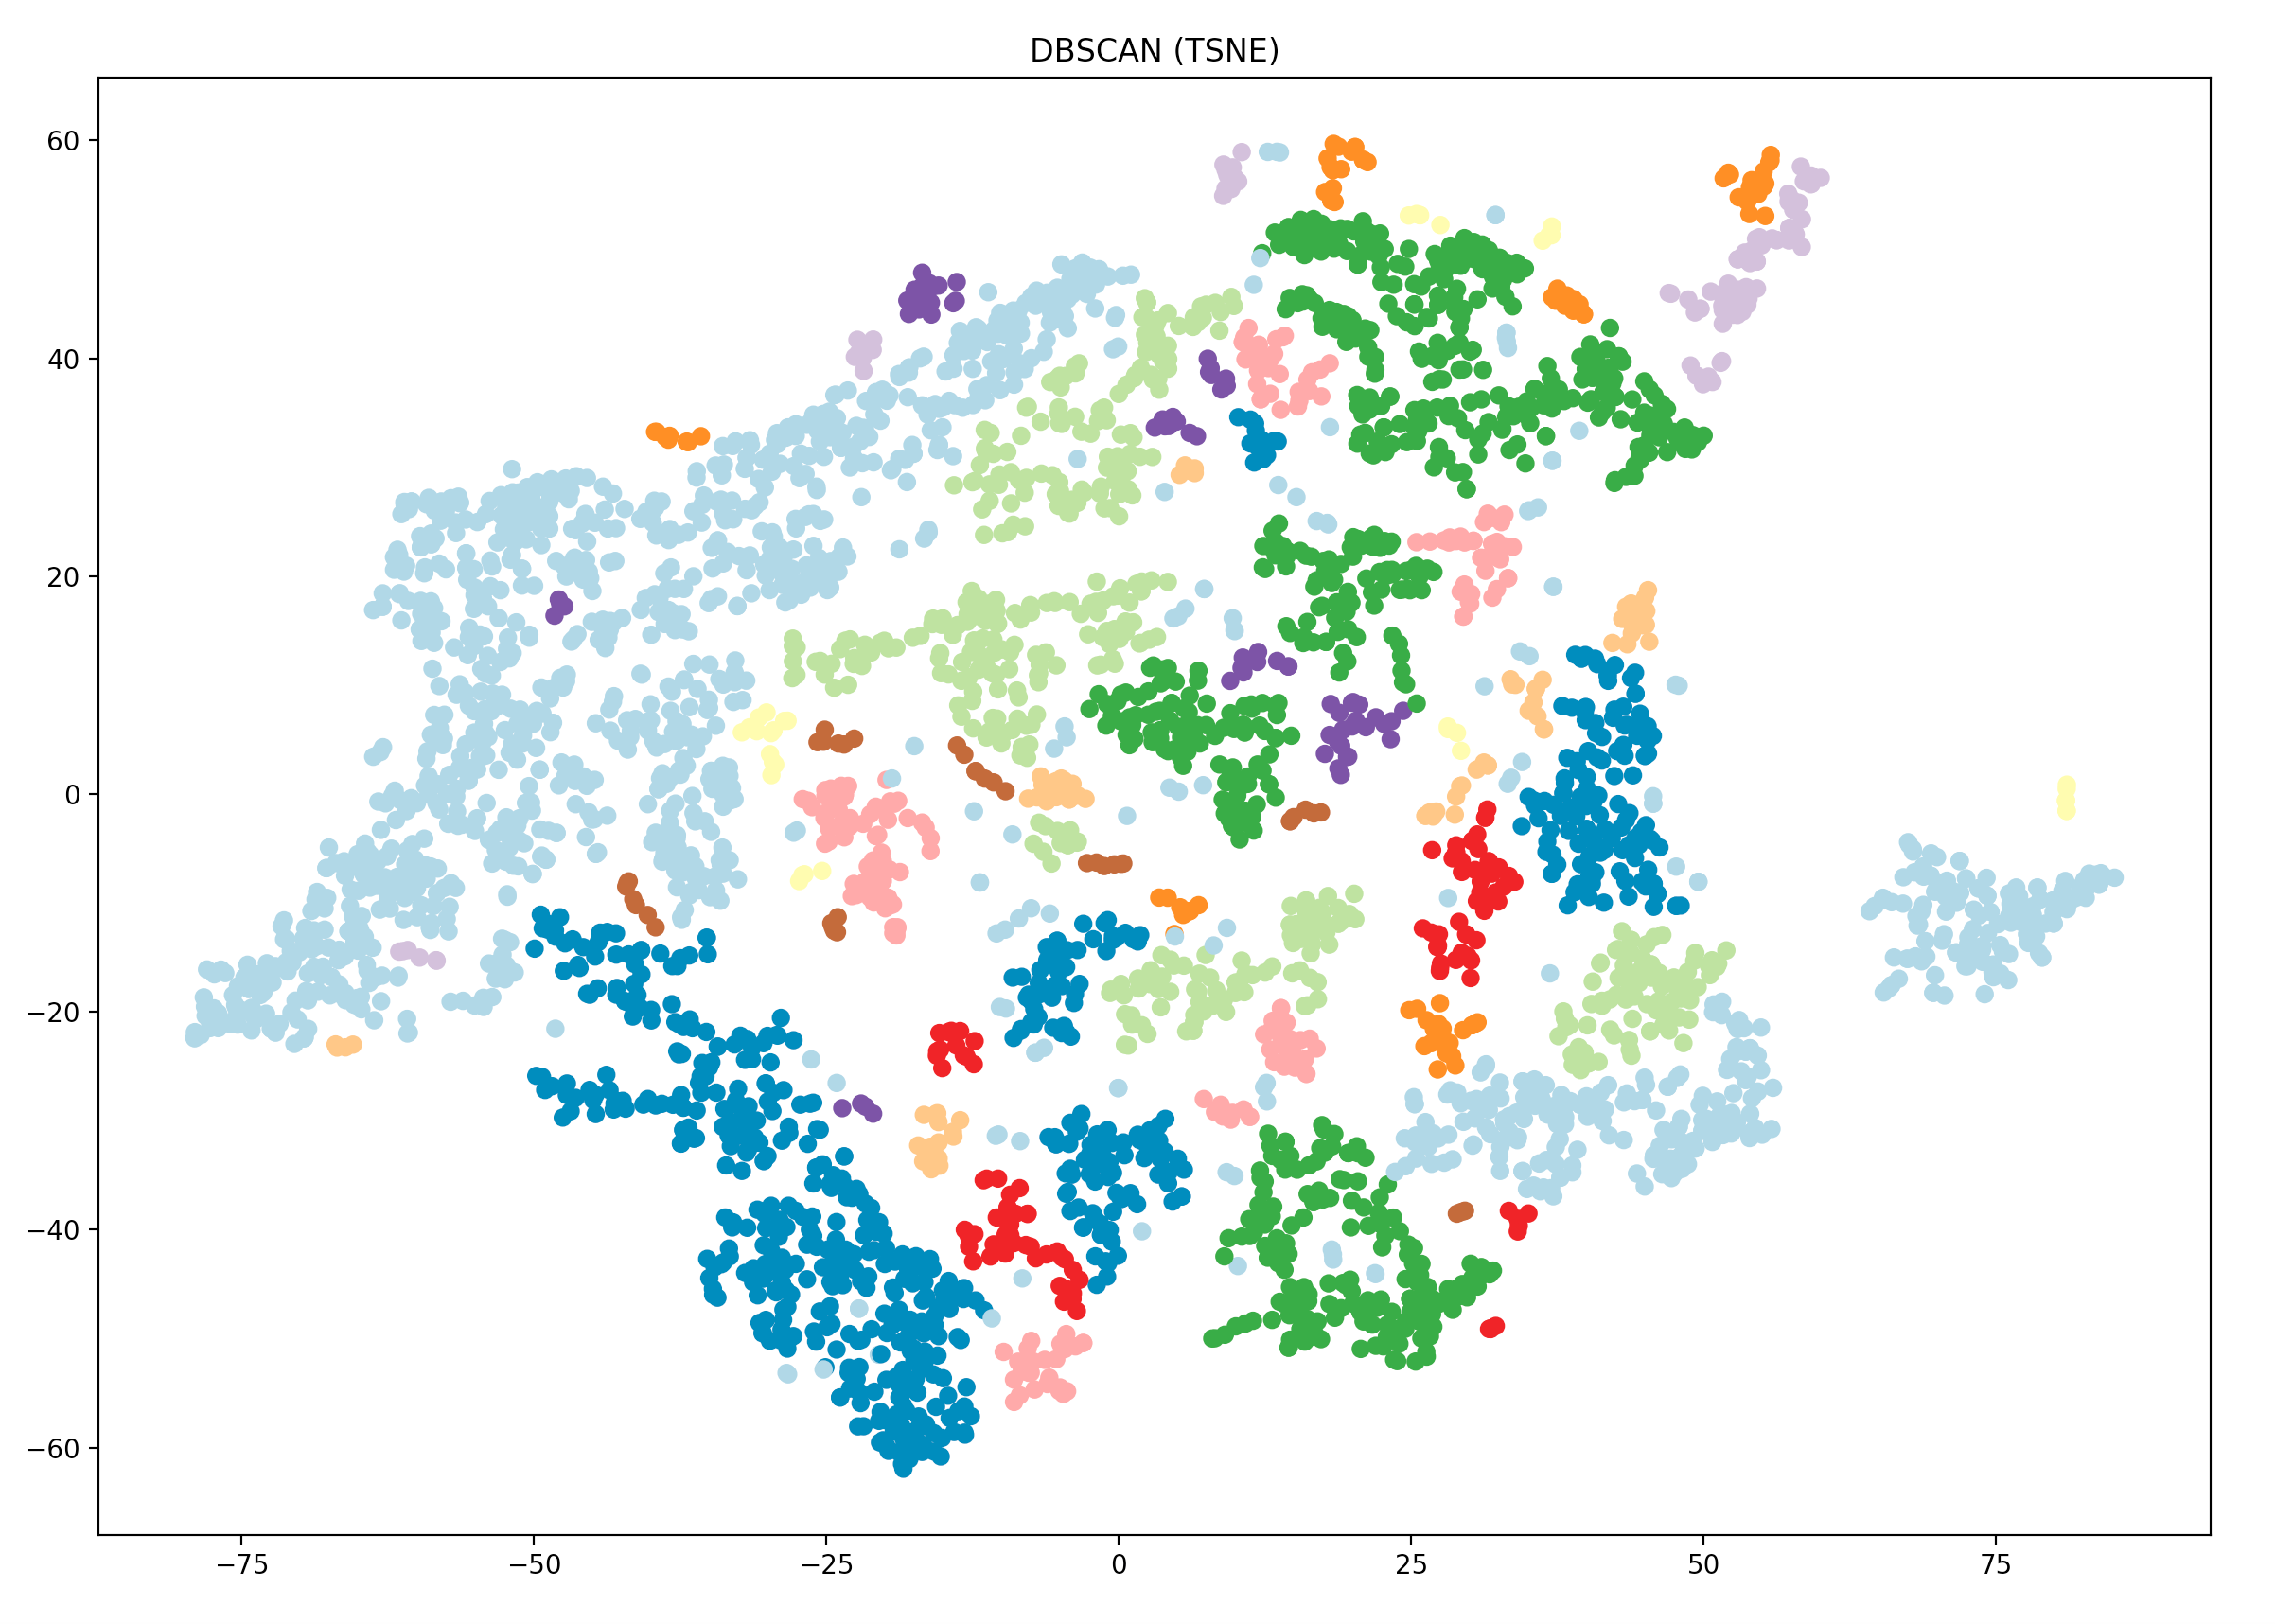
\includegraphics[width=0.9\textwidth]{./images/tsneParametersTest/perplexity/perp45-3hDBSCAN.png}
    % \caption{}
    % \label{figure:}
	\end{subfigure}
	\caption{\textbf{3h} data files, t-SNE calculated with the following parameters: \textbf{perplexity=45}, n\_iter=5000, learning\_rate=50}
  \label{figure:3hperp45TSNE}
\end{figure}



%------------------ PERPLEXITY 50: ------------------
\subsubsection{Perplexity = 50}
% -- 1h, perp 50 --
\begin{figure}[H]
  \centering
  \begin{subfigure}{.5\textwidth}
    \centering
    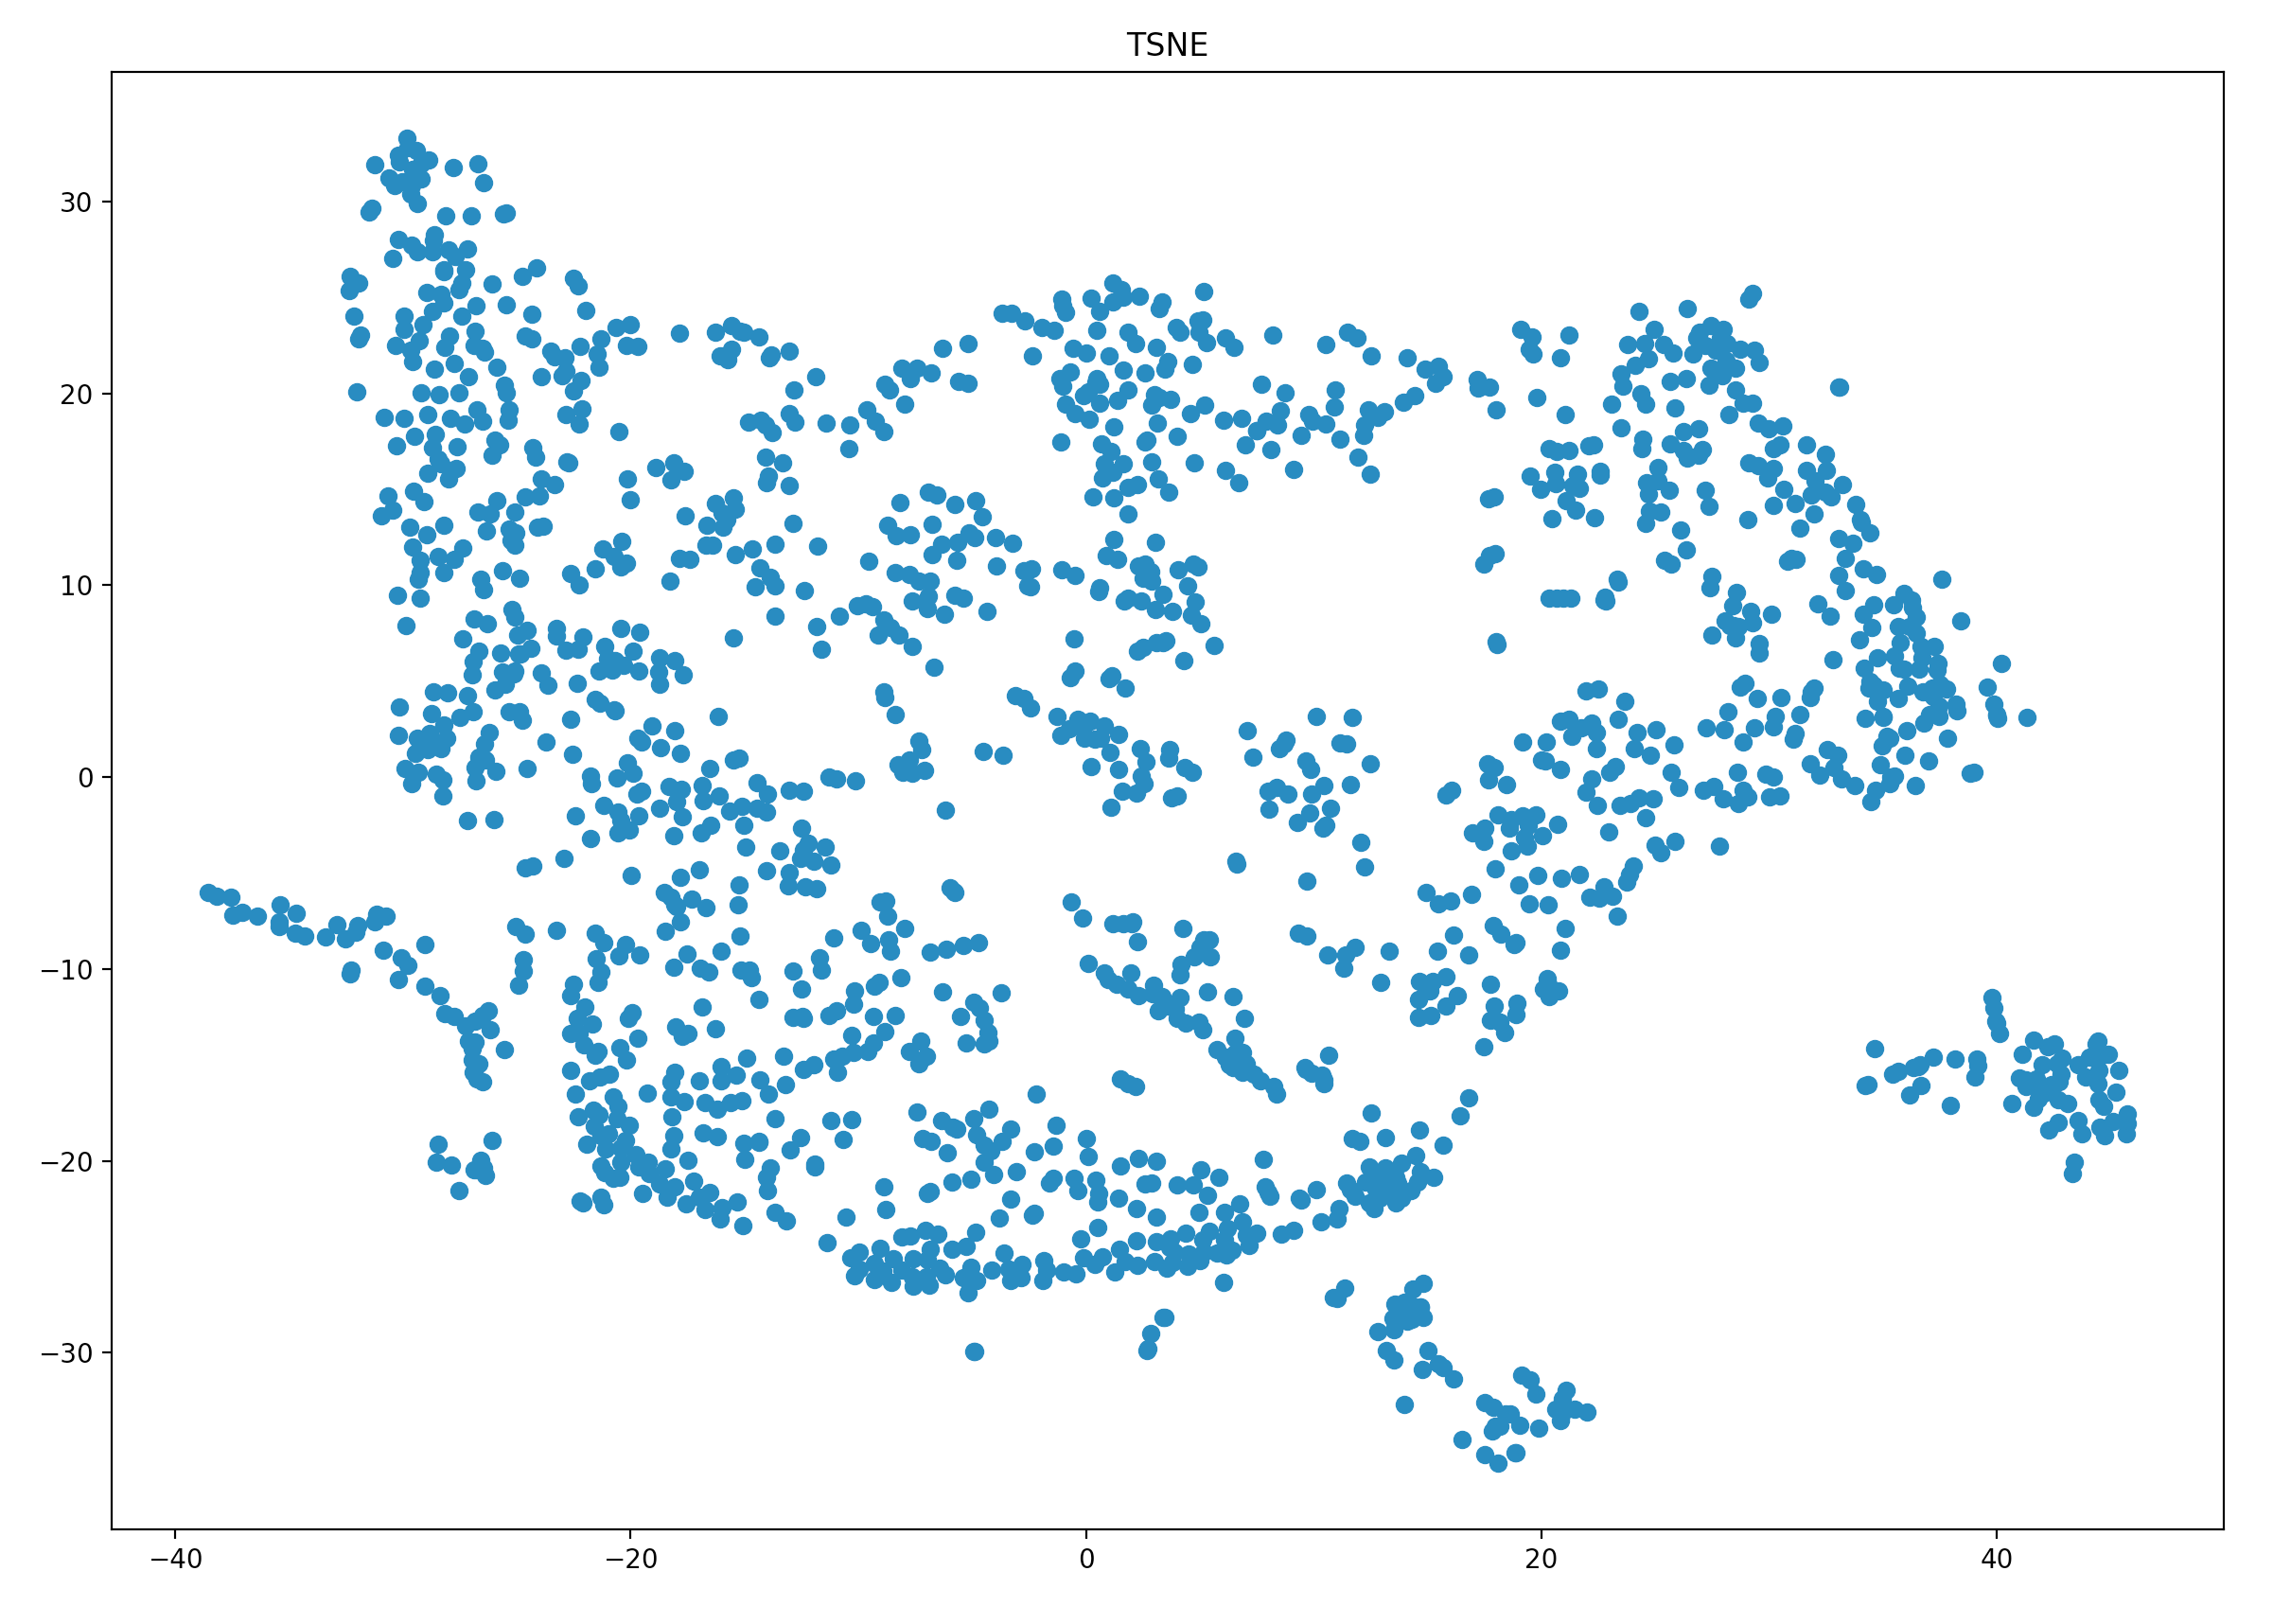
\includegraphics[width=0.9\textwidth]{./images/tsneParametersTest/perplexity/perp50-1hTSNE.png}
  % \caption{}
  % \label{figure:}
  \end{subfigure}%
  \begin{subfigure}{.5\textwidth}
    \centering
    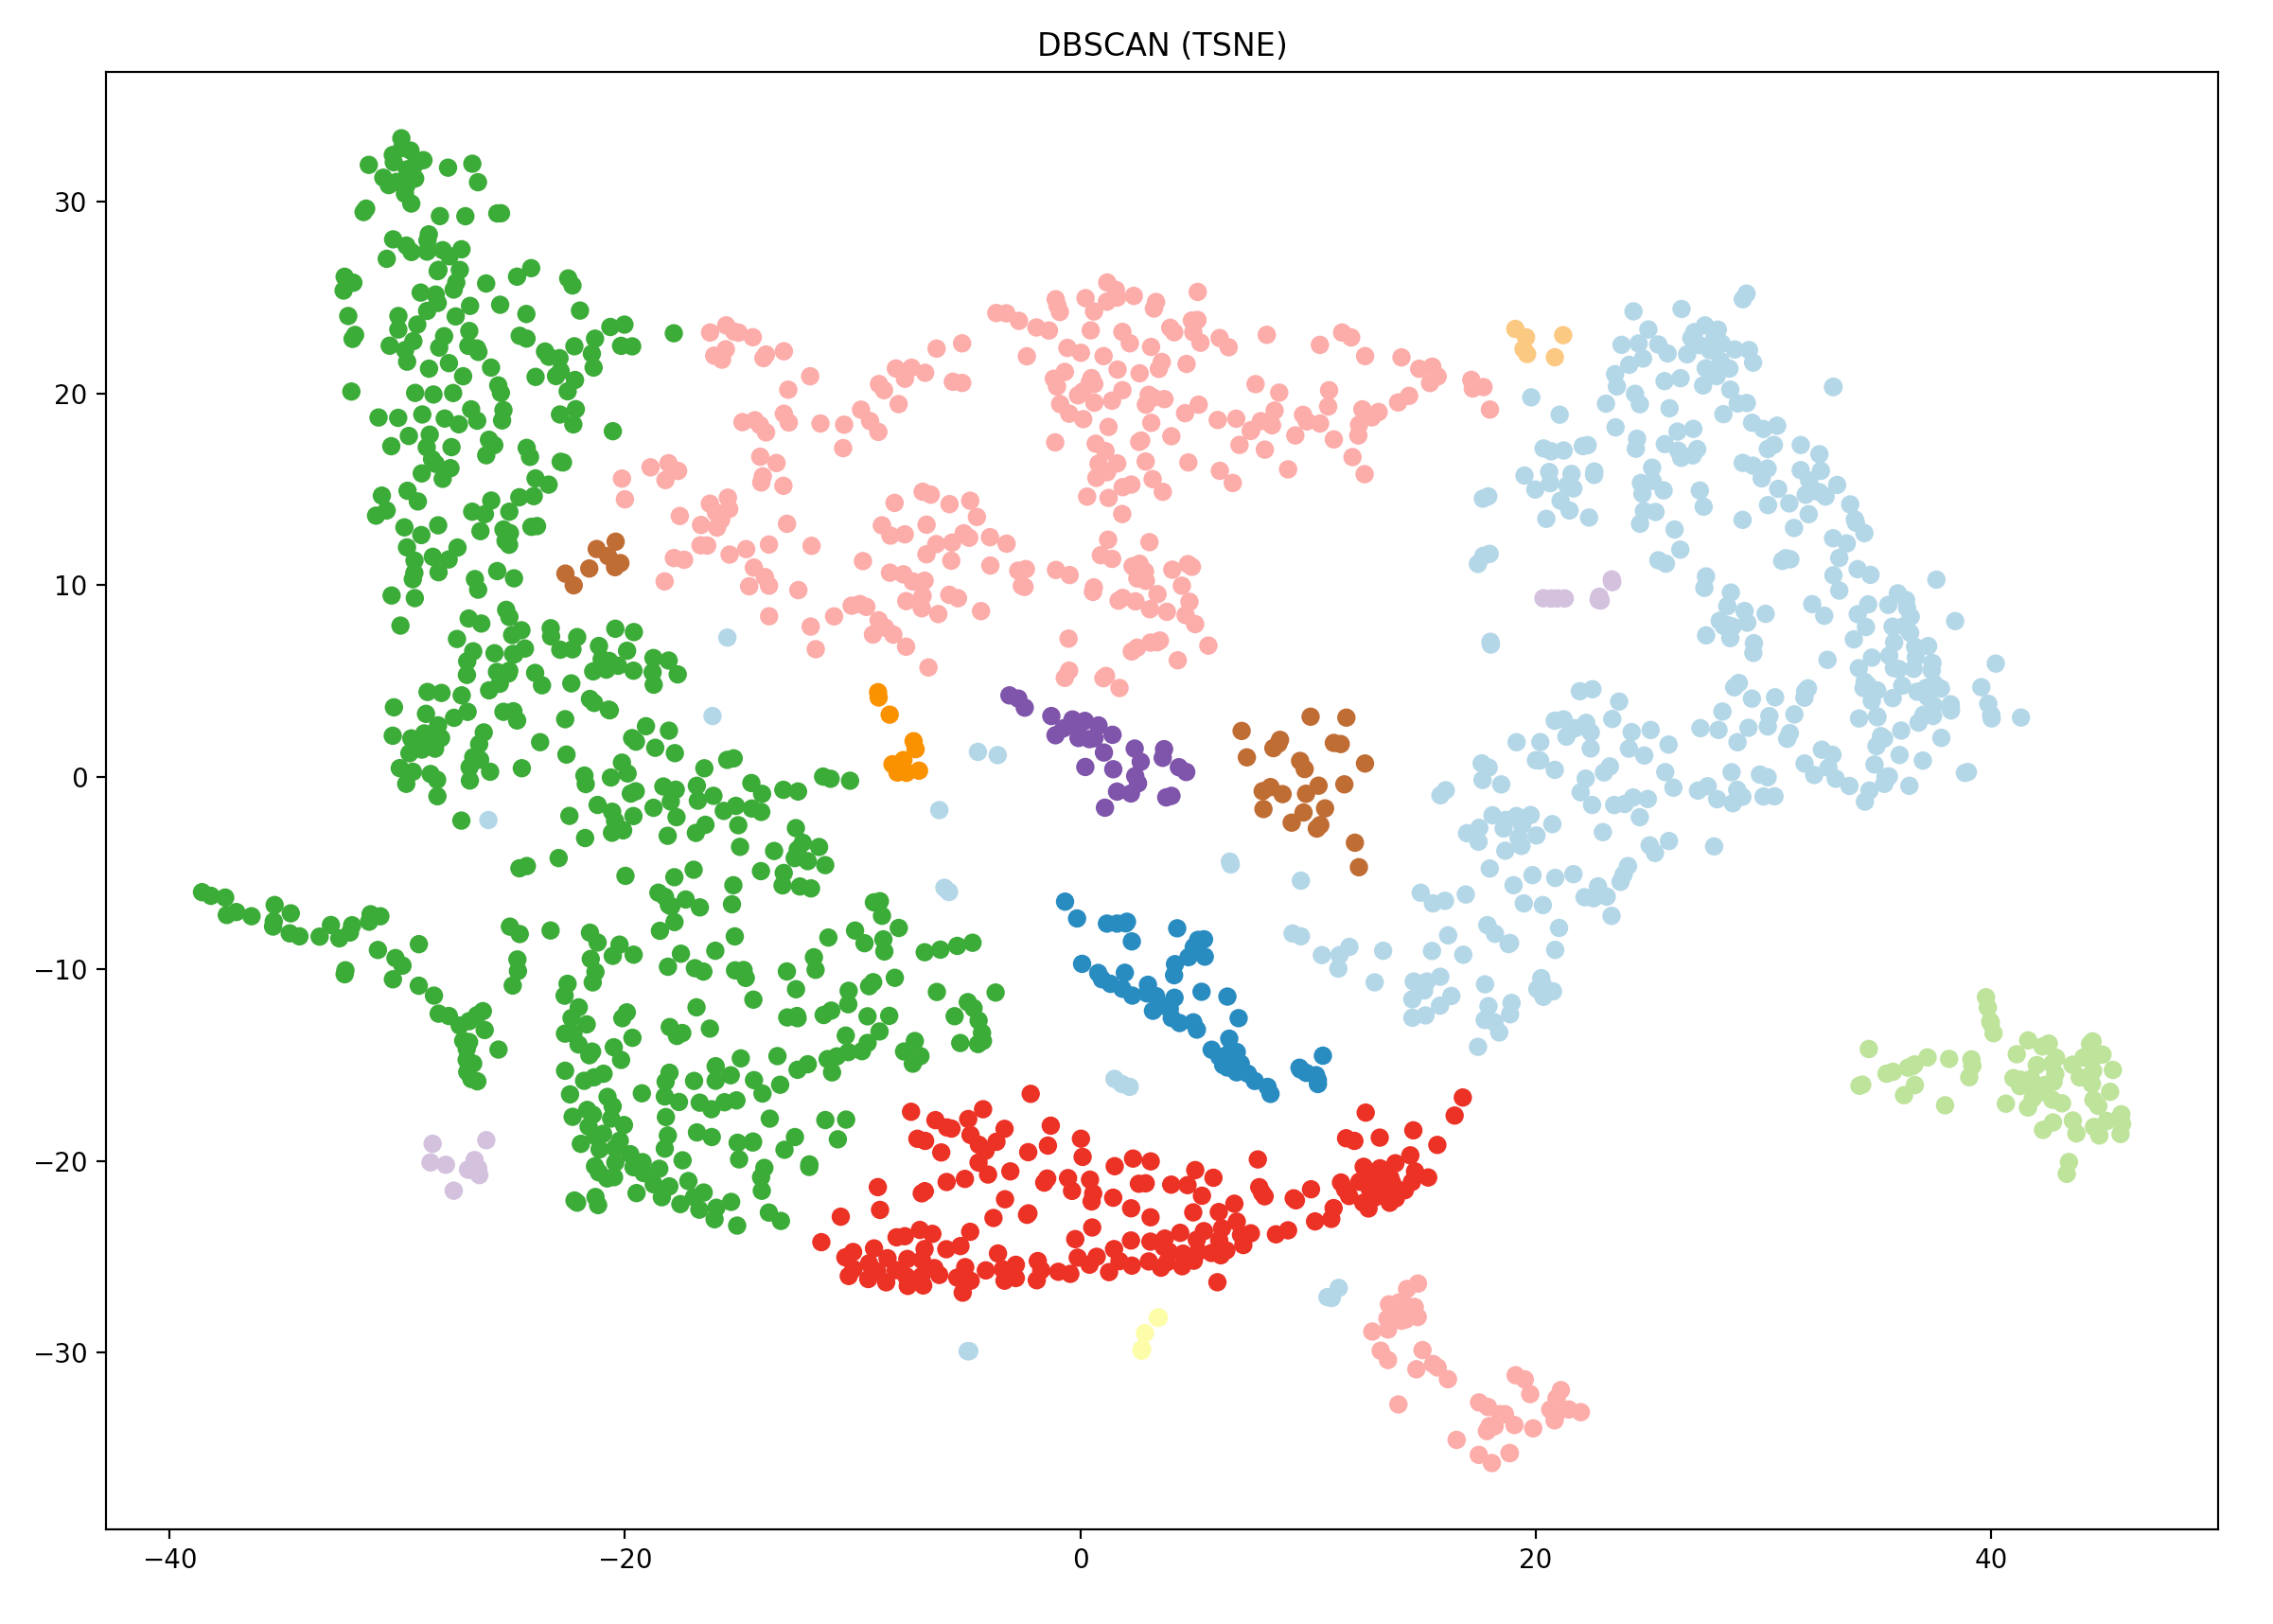
\includegraphics[width=0.9\textwidth]{./images/tsneParametersTest/perplexity/perp50-1hDBSCAN.png}
    % \caption{}
    % \label{figure:}
  \end{subfigure}
	\caption{\textbf{1h} data files, t-SNE calculated with the following parameters: \textbf{perplexity=50}, n\_iter=5000, learning\_rate=50}
  \label{figure:1hperp50TSNE}
\end{figure}

% -- 3h, perp 50 --
\begin{figure}[H]
  \centering
	\begin{subfigure}{.5\textwidth}
    \centering
    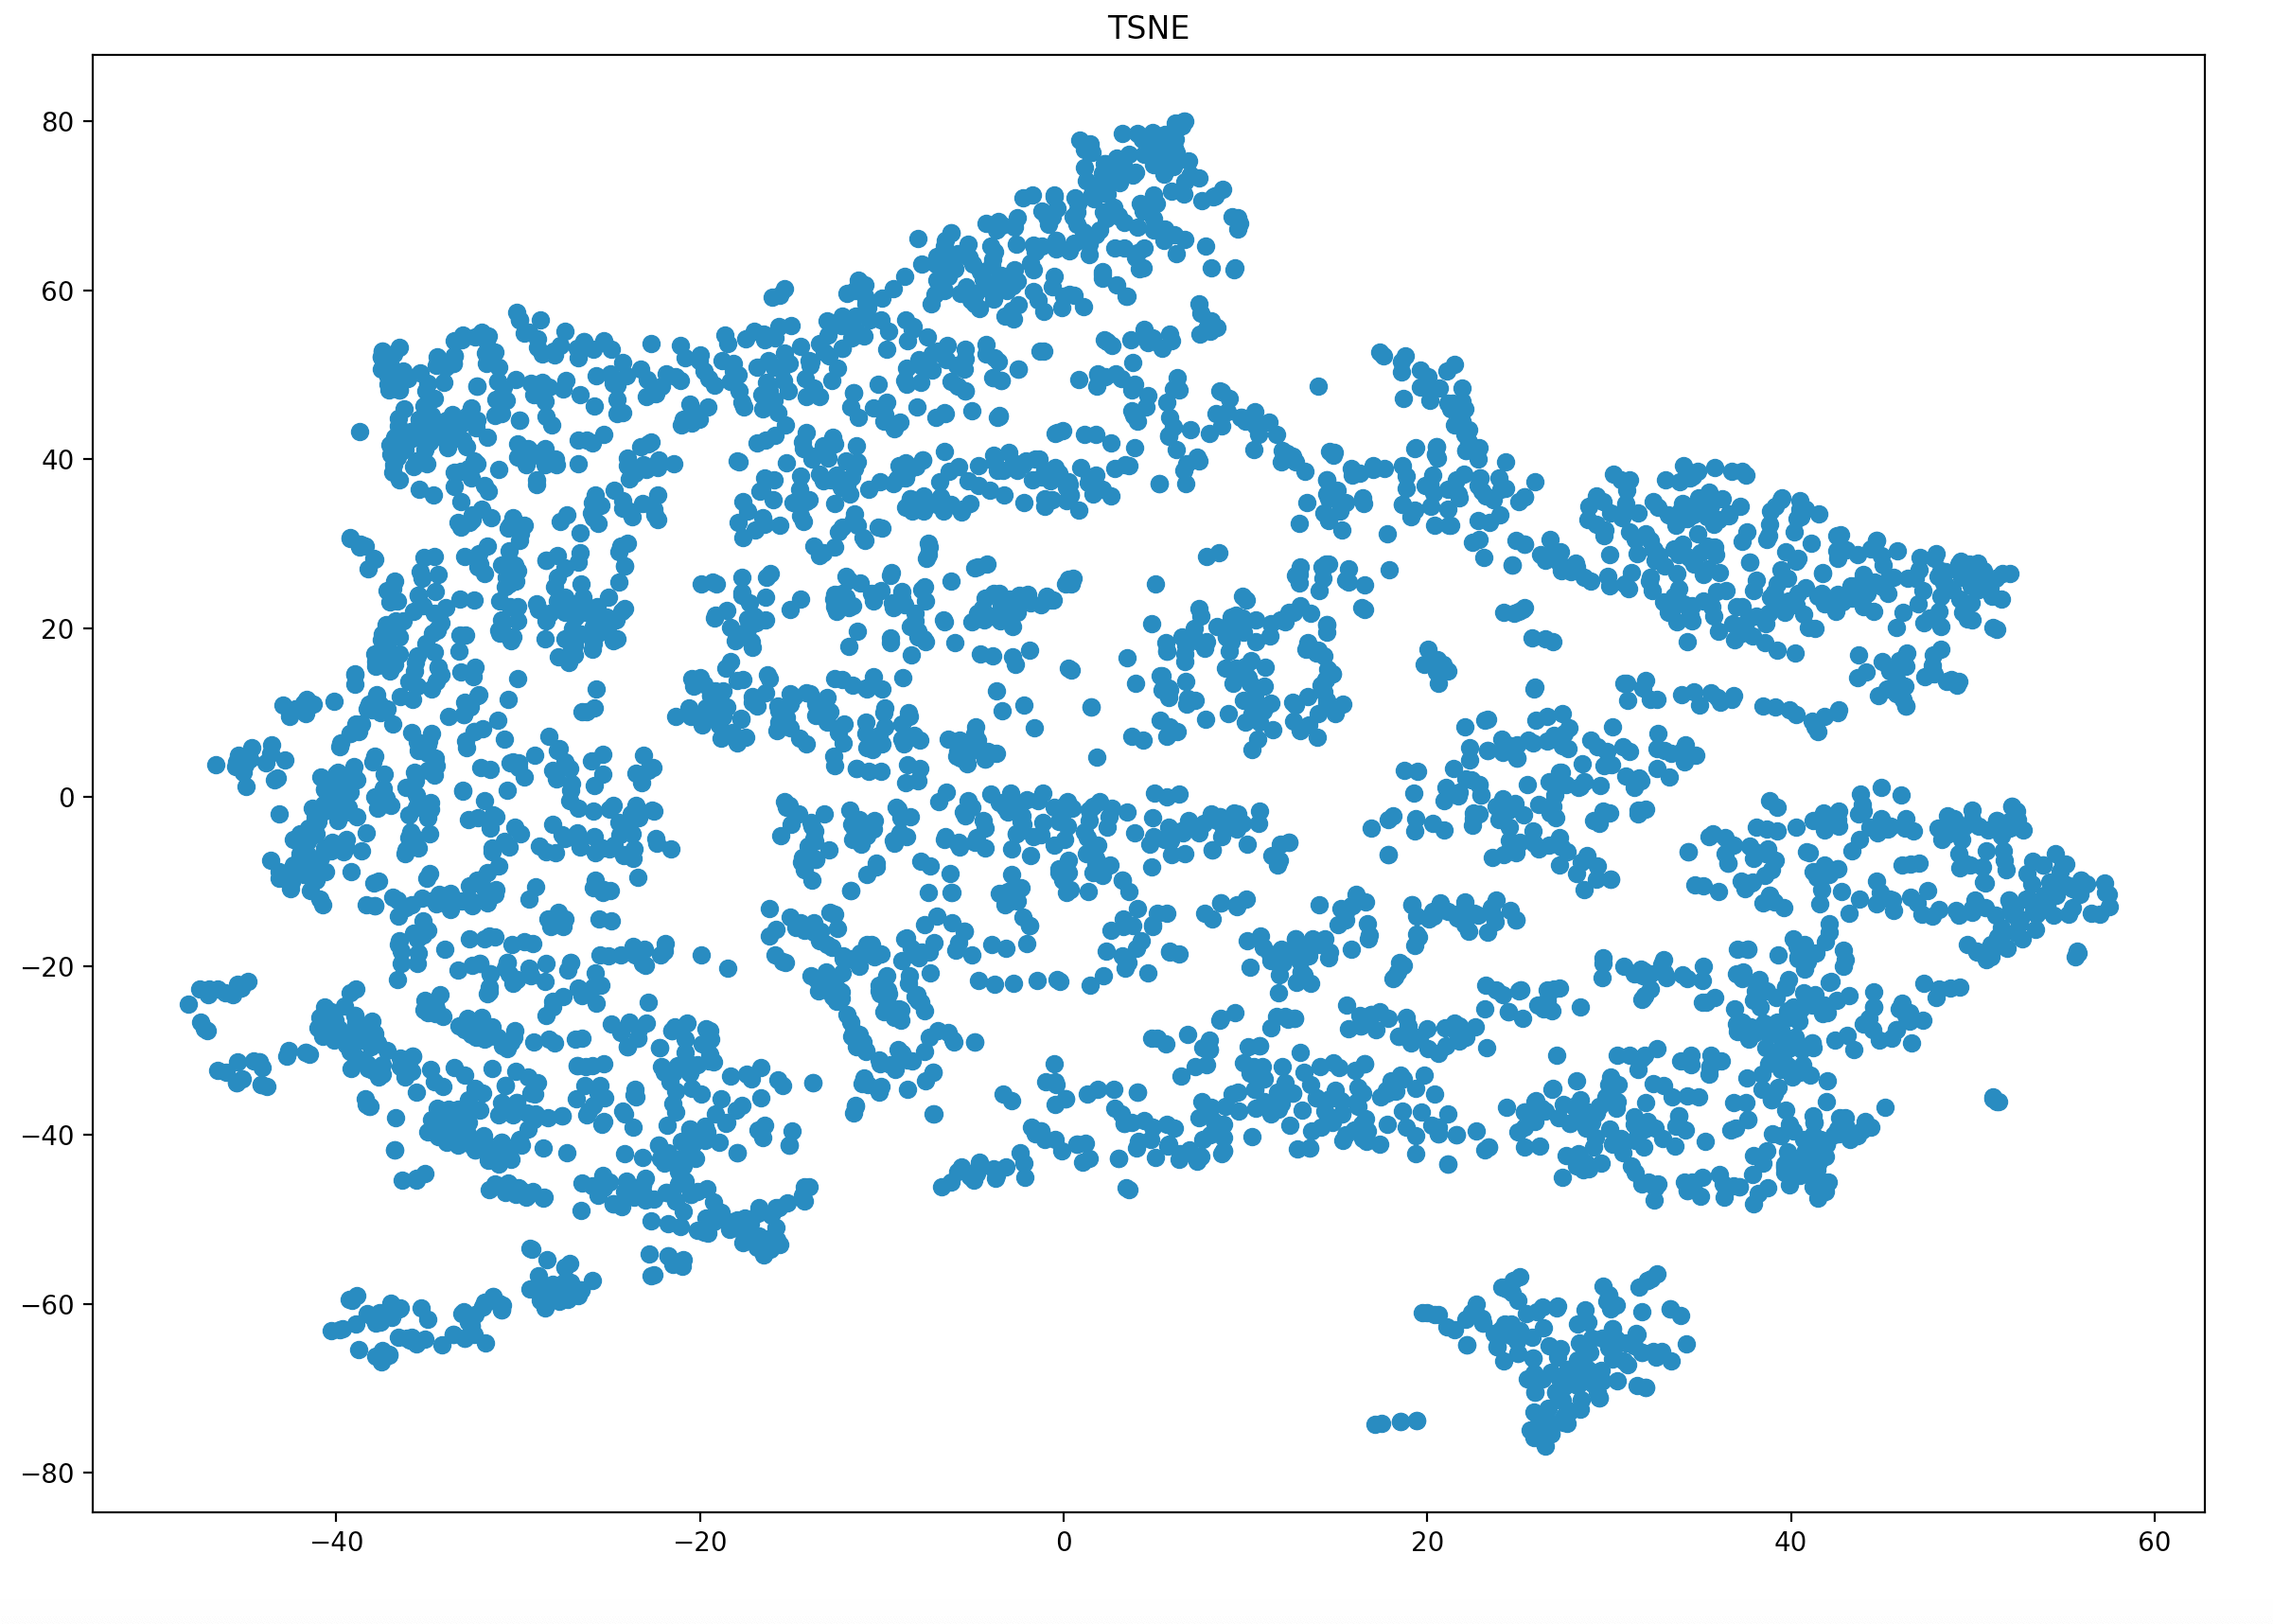
\includegraphics[width=0.9\textwidth]{./images/tsneParametersTest/perplexity/perp50-3hTSNE.png}
  % \caption{}
  % \label{figure:}
  \end{subfigure}%
  \begin{subfigure}{.5\textwidth}
    \centering
    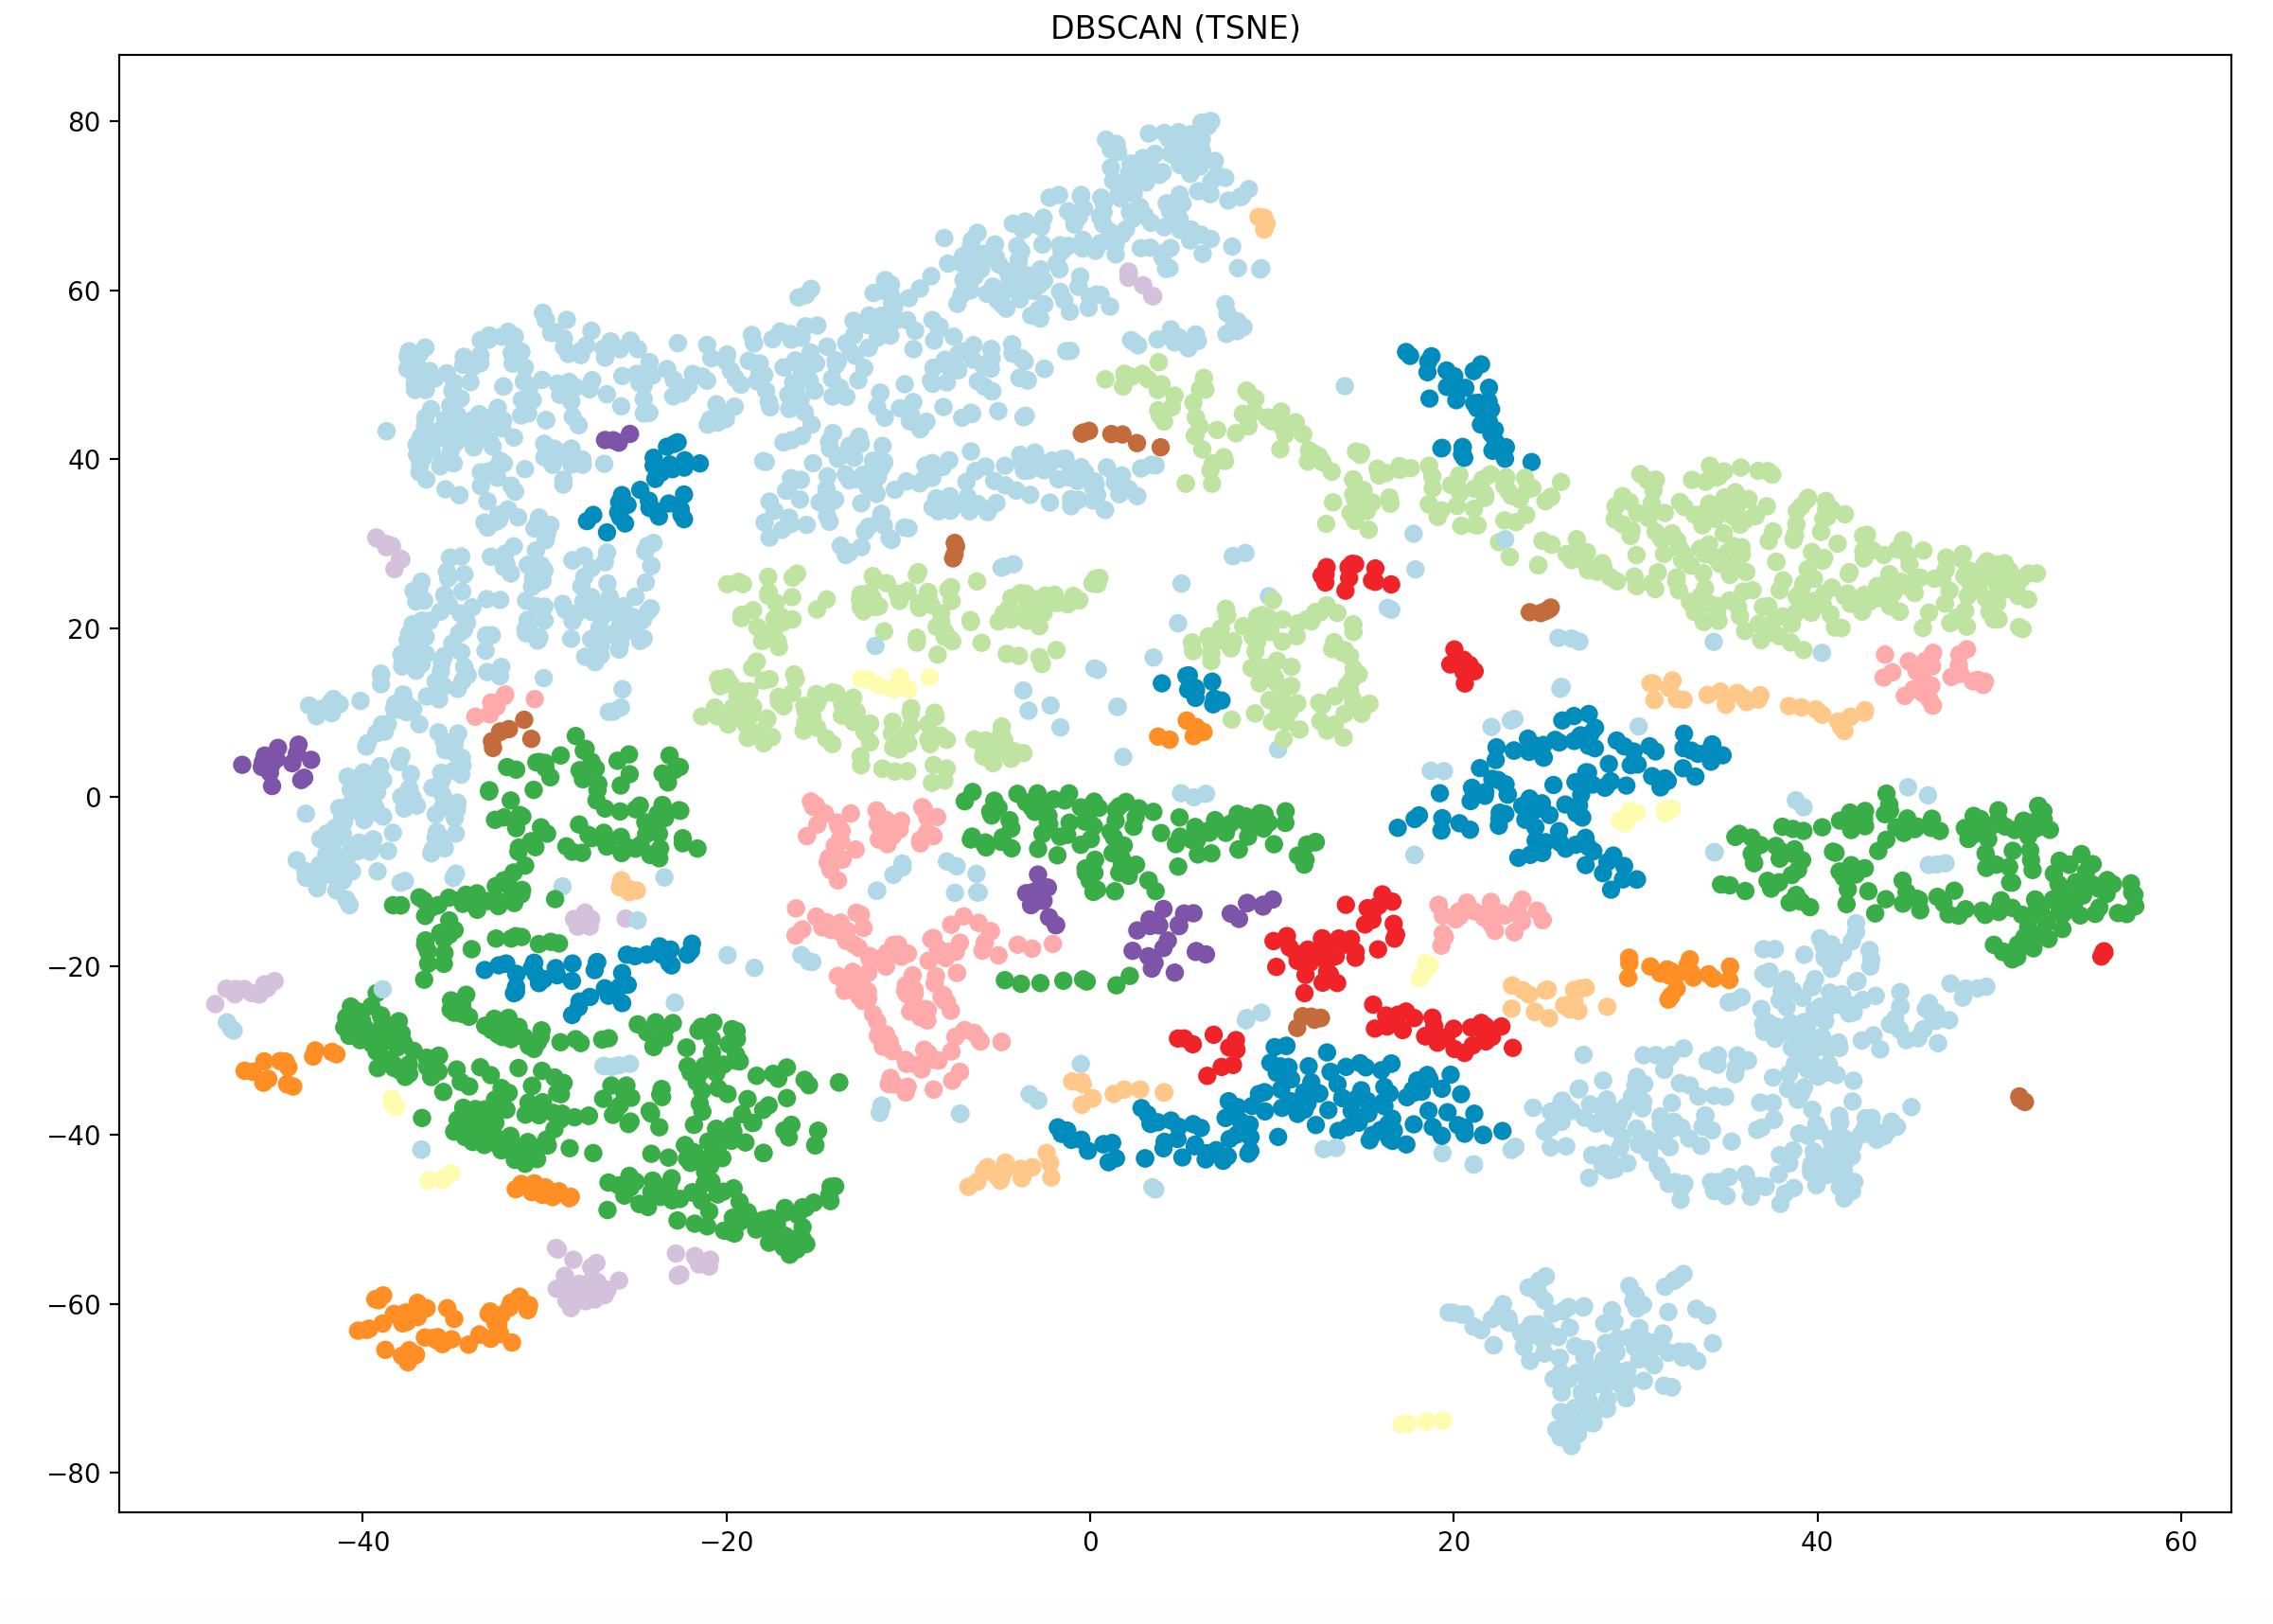
\includegraphics[width=0.9\textwidth]{./images/tsneParametersTest/perplexity/perp50-3hDBSCAN.png}
    % \caption{}
    % \label{figure:}
	\end{subfigure}
	\caption{\textbf{3h} data files, t-SNE calculated with the following parameters: \textbf{perplexity=50}, n\_iter=5000, learning\_rate=50}
  \label{figure:3hperp50TSNE}
\end{figure}





\subsubsection{Perplexity Comparison Results (Average of two different t-SNE runs)}
\label{appendix:compareAveragePerplexity}

\begin{figure}[H]
  \centering
  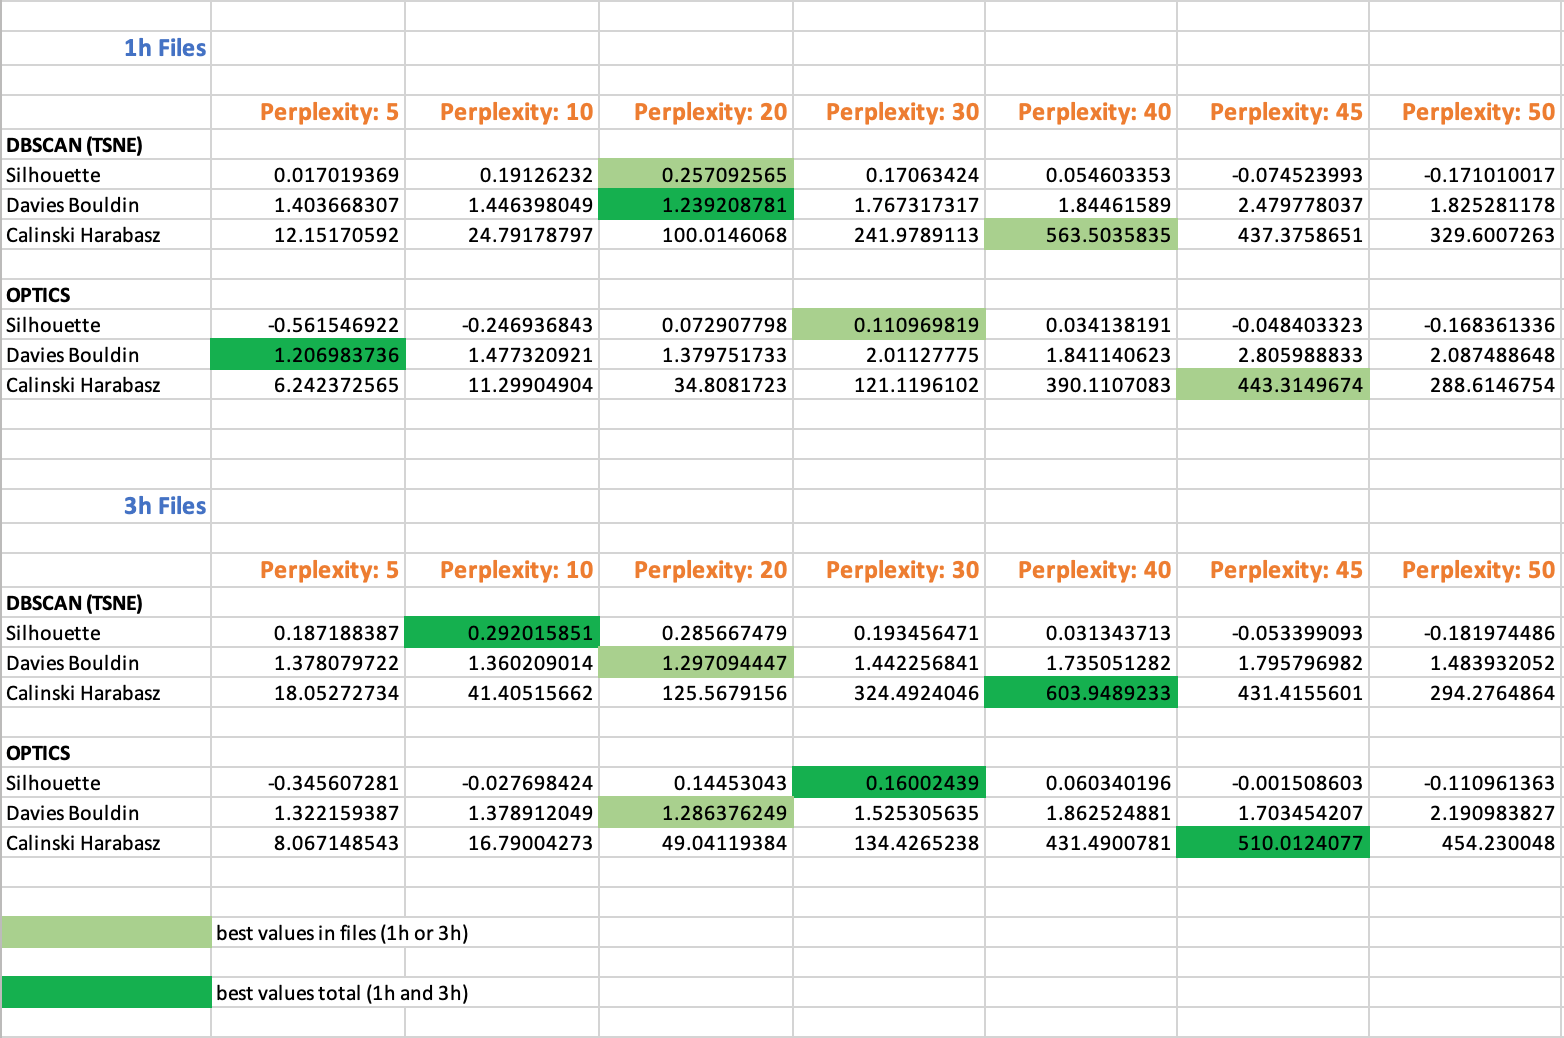
\includegraphics[width=0.8\textwidth]{./images/tsneParametersTest/perplexity/perplexityEvaluationScoresAverage.png}
  \caption{Comparison of Silhouette Coefficient, Davies-Bouldin Index, and Caliński-Harabasz Index for different t-SNE \textbf{perplexities}. The lighter green highlighted values indicate the best values of that file aggregation (1h or 3h files). The dark green highlighted values illustrate the overall best values over all files (1h and 3h files).}
  \label{figure:perplexityEvaluationScoresAverage}
\end{figure}

\begin{figure}[H]
  \centering
  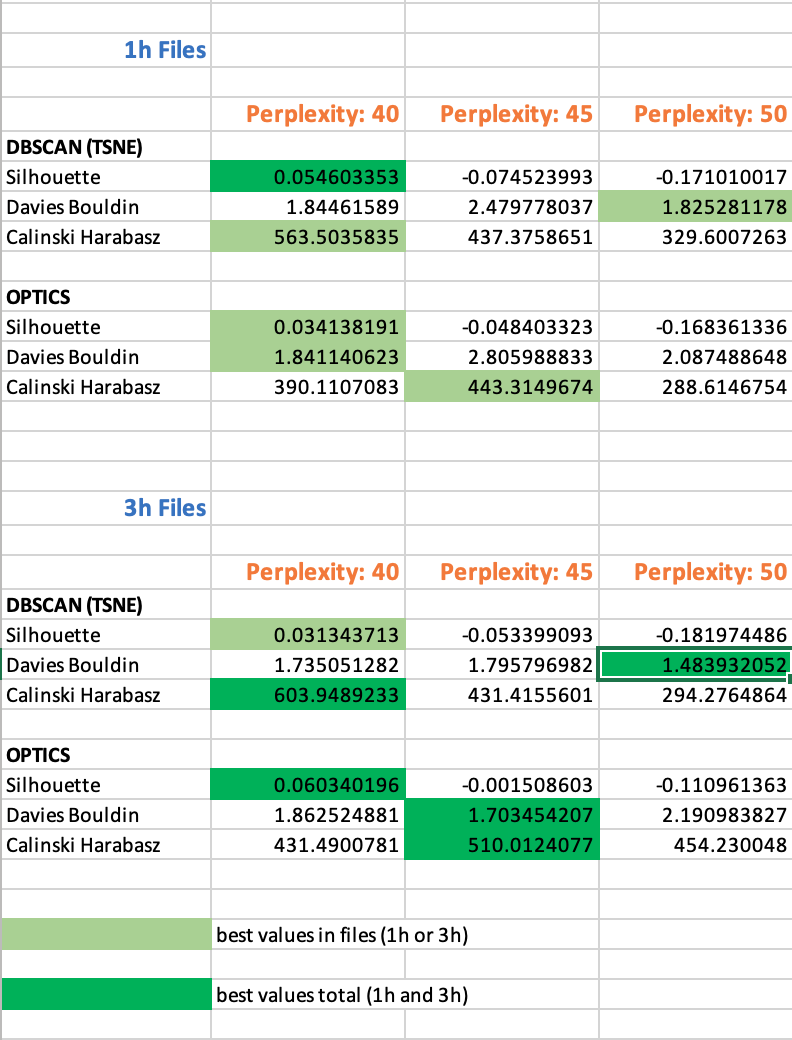
\includegraphics[width=0.4\textwidth]{./images/tsneParametersTest/perplexity/perplexityEvaluationScoresDetailedAverage.png}
  \caption{Comparison of Silhouette Coefficient, Davies-Bouldin Index, and Caliński-Harabasz Index for different t-SNE \textbf{perplexities}. The lighter green highlighted values indicate the best values of that file aggregation (1h or 3h files). The dark green highlighted values illustrate the overall best values over all files (1h and 3h files).}
  \label{figure:perplexityEvaluationScoresDetailedAverage}
\end{figure}


\clearpage